\documentclass[12pt]{article}
\usepackage[utf8]{inputenc}
\usepackage{gensymb}
\usepackage{titlesec}
\usepackage{graphicx}
\usepackage{booktabs}
\usepackage{wrapfig}
\usepackage{mathtools}
\usepackage[export]{adjustbox}
\usepackage{algorithm}
\usepackage{algpseudocode}
\usepackage{listings}
\usepackage{afterpage}
\usepackage{url}
\setcounter{secnumdepth}{4}
\makeindex
\pagestyle{empty}
\usepackage[left=1.5cm,top=2.5cm,right=1.5cm,bottom=2.5cm]{geometry} %margenes supuestamente
\begin{document}
\null\newpage
\afterpage{\null\newpage}
%titlepage
\thispagestyle{empty}
\begin{center}
\begin{minipage}{0.75\linewidth}
    \centering
%University logo
    
\includegraphics[width=0.3\linewidth]{logofing.png}
    \\Instituto de Computación 
    \\Facultad de Ingeniería Universidad de la República
	\\Montevideo – Uruguay\\
    \vspace{1cm}
%Thesis title
    {\uppercase{\Large Visualización Estereoscópica de Ecuaciones Implícitas\par}}
    \vspace{3cm}
%Author's name
    {\Large Guillermo Báez\\Pablo Coore\par}
    \vspace{1cm}
    Tutor: Eduardo Fernández\\
    \vspace{2cm}
%Degree
    {\Large Proyecto de Grado\par}
    \vspace{3cm}
%Date
    {\Large Mayo 2016}
\end{minipage}
\end{center}


\pagestyle{plain}
\renewcommand{\figurename}{Figura}
\renewcommand{\tablename}{Tabla}
\renewcommand{\contentsname}{Índice}

\section*{Resumen}
La visualización espacial de ecuaciones es una tarea compleja para estudiantes en todas las etapas de la formación académica. Gran parte del análisis matemático está dedicado a determinar las principales características de las  funciones matemáticas, como punto de partida para lograr su comprensión y entendimiento.

La propuesta de este trabajo consiste en implementar un programa que permita la visualización de ecuaciones implícitas, utilizando tecnologías gráficas relacionadas con la visión estereoscópica.  Con esto se busca acercar al estudiante los componentes estéticos y visuales de las matemáticas. Además se quiere obtener una experiencia de realidad virtual agradable al usuario.
%XXX dice que este parrafo es poco claro, volver a escribirlo
En el marco de este proyecto, se concluyó que los algoritmos basados en la generación de mallas son más adecuados para la visualización estereoscópica debido a que tiene un mejor tiempo de respuesta a la hora de actualizar la posición de la cámara.

Por último, se cuenta con una aplicación web\footnote{El código fuente se encuentra disponible en \cite{nuestrocodigo} y se puede acceder a la aplicación en \cite{nuestrositio}}, que funciona  tanto en PC como en celulares, siendo ésta compatible con Oculus Rift (DK1, DK2 y Consumer Version) si se utiliza Nightly, y con Google Cardboard en celulares.
\\
\\
\\
\\
\textbf{Palabras clave:} \textit{Oculus Rift, THREEJS, Javascript, WebGL, GLSL, visualización de ecuaciones} 


\clearpage
\tableofcontents
\clearpage
\section{Introducción}

\subsection{Definición del problema y motivación}
La visualización espacial de curvas y superficies matemáticas es un reto importante para estudiantes y docentes. Gran parte del análisis matemático está dedicado a determinar las principales características, puntos singulares, pendientes, concavidades y demás características de las  funciones matemáticas, como punto de partida para lograr su comprensión y entendimiento.
\\En los últimos años se han desarrollado paquetes de software que facilitan la visualización computacional de diversos tipos de ecuaciones. Los paquetes de cálculo científico poseen herramientas de visualización poderosas que hacen posible graficar de forma intuitiva un volumen importante de información compleja\footnote{Por ejemplo Gnuplot es una herramienta libre ampliamente utilizada en el ámbito científico para la visualización de funciones matemáticas y se puede encontrar en \\\texttt{http://www.gnuplot.info/}\cite{gnuplot}.}.  
\\En el área de la educación, actualmente hay experiencias exitosas, como Surfer\cite{surfer}, 3DXplorMath\cite{dxplormath}, entre otros, que permiten al estudiante introducirse en el mundo de la abstracción geométrica. 
\\Además la visualización de superficies y curvas tridimensionales son ampliamente utilizadas en varias disciplinas para la visualización de datos: química, geofísica, meteorología y dinámica de los fluidos, permitiéndole a los ingenieros estudiar características de los mismos mediante simulaciones. Por ejemplo, se puede estudiar el flujo del viento a través de un modelo por computadora de una ala de avión \cite{aircraftwing}. 
\\En este contexto, se quieren explorar las posibilidades de desarrollar una aplicación para que sea posible visualizar de forma estereoscópica e interactiva (en tiempo real) curvas y superficies matemáticas. Para ello la idea es considerar el uso del dispositivo de visualización Oculus Rift, y de hardware gráfico (tarjetas gráficas) Nvidia.
\subsection{Objetivos}
\begin{itemize}
\item Desarrollar una aplicación para visualizar ecuaciones algebraicas de forma estereoscópica y en tiempo real.
\item Aprender a utilizar el dispositivo Oculus para la visualización estereoscópica. 
\item Incorporar nuevas facilidades de construcción de superficies, como el uso de operadores booleanos (Geometría Sólida Constructiva). 
\item Estudiar y desarrollar formas interesantes de visualización y recorrido de las superficies.
\item Que la aplicación desarrollada esté disponible para su compilación y ejecución por terceros. 
\end{itemize}
\subsection{Resultados Esperados}
\begin{itemize}
\item Un sitio web desde donde se describan las principales características del software y se tenga acceso al paquete desarrollado para su instalación en equipos de terceros. 
\item Un artículo y póster con las principales características del proyecto, para su presentación en actividades académicas.
\end{itemize}

\clearpage
\section{Estado del Arte}
En esta sección se hará una breve introducción a una serie de conceptos y tecnologías que son la base del proyecto. La primer sección trata sobre las definiciones de los distintos tipos de superficie, esto sirve de introducción para la explicación que se encuentra en la próxima sección sobre dos técnicas para la visualización de un tipo de superficies en particular. 
\\Más adelante se presenta una serie de programas que se utilizan con el fin de visualizar superficies, así como un breve análisis de los mismos.
\\Luego se muestra una serie de conceptos y hardware para lograr una visualización estereoscópica. A continuación se listan varios paquetes de software que fueron utilizados en la realización de la aplicación que se obtuvo como resultado del proyecto.
\\Finalmente se realiza un resumen acerca de un fenómeno que se puede experimentar si se presentan determinadas condiciones cuando se está trabajando con visualización estereoscópica.
\subsection{Tipos de superficies}
En matemáticas una superficie implícita es una superficie en el espacio euclidiano definida por una ecuación $F (x, y, z) = 0$.
\\Es decir, una superficie implícita es el conjunto de puntos a los cuales aplicarle una función de 3 variables da cero. 
\\La gráfica de una función se describe generalmente por una ecuación $z = f (x, y)$ y se llama una representación explícita\cite{implicitas}\cite{realtimerendering}. La tercera descripción esencial de una superficie es la paramétrica: $(x(s, t), y (s, t), z (s, t))$, donde las coordenadas de los puntos $x$, $y$, $z$ son representadas por tres funciones $x(s, t), y(s, t) , z(s, t)$ dependiendo de los parámetros que tienen en común ($s$ y $t$).
\\Ejemplos de superficies implícitas:
\\Tetraedro: $max(max(max(x + y - z - 1, -x + y + z - 1), x - y + z -1), -x - y - z - 1) = 0$
\\Plano $x = 0$.
\\Esfera  $x^2 +y^2 +z^2 - 4 = 0$.
\\Superficie de género:  $2y (y^2 -3x^2) (1-z^2) + (x^2 +y^2)2- (9z^2-1) (1-z^2) =0$ 
\\Superficie de revolución (copa de vino) $x^2 + z^2 - 2(- ln (y+ 3,5)) - 0,02 = 0$
\begin{figure}[ht]
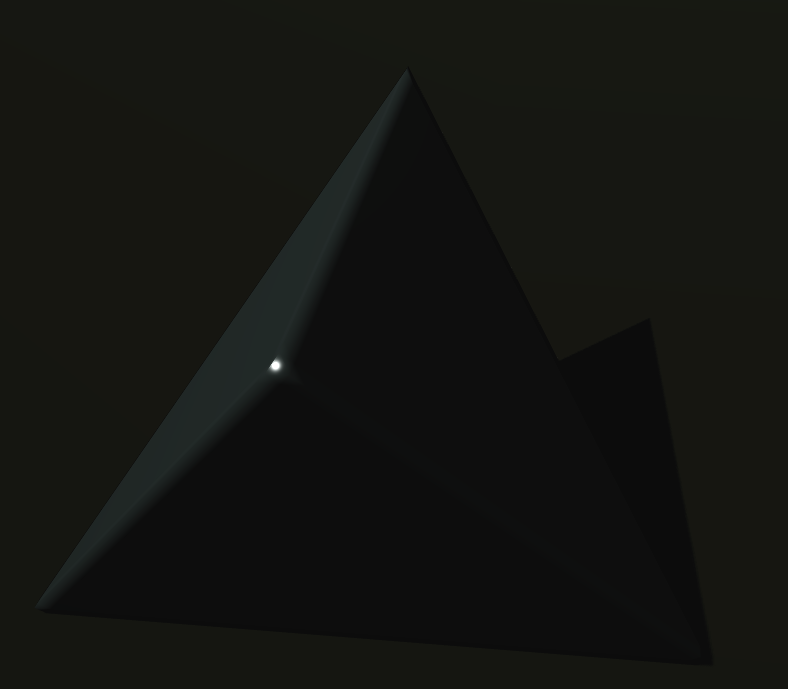
\includegraphics[width =0.45\linewidth]{tetraedro.png}
\hfill
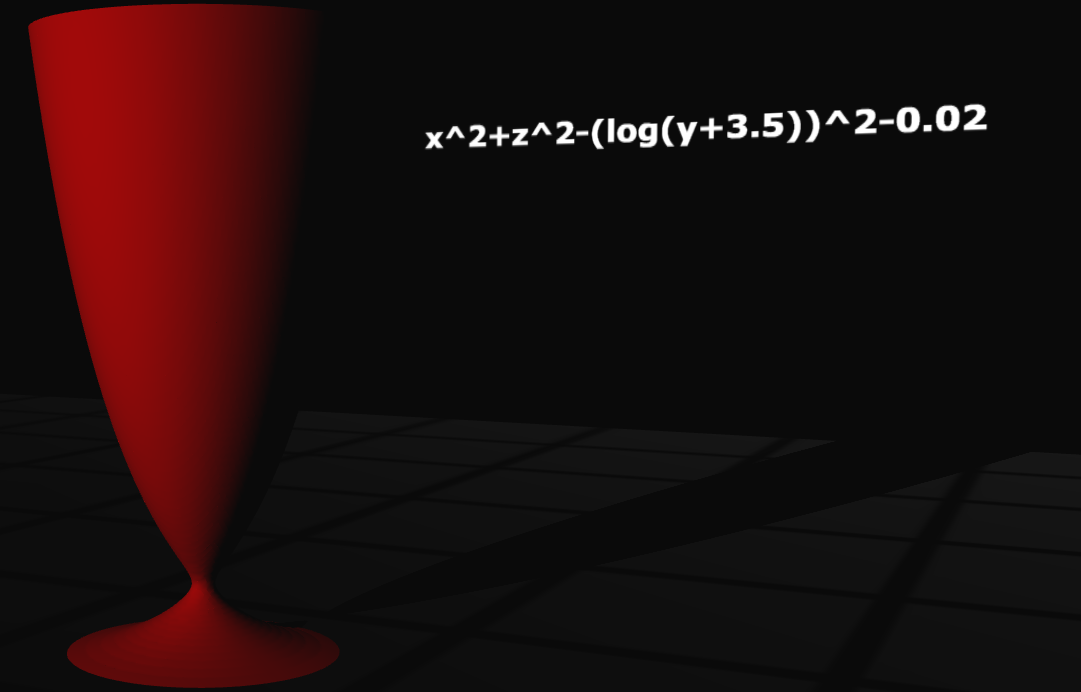
\includegraphics[width =0.45\linewidth]{copa.png}
\caption{ Un tetraedro y una superficie de revolución generados con la aplicación desarrollada.}
\label{ fig : surface }
\end{figure}
\\Para un plano, una esfera y un toro existen representaciones paramétricas simples. Esto no es cierto para todos los casos de superficies implícitas.
\\El teorema de la función implícita\footnote{Para más información sobre este teorema ver el anexo A.} describe las condiciones bajo las cuales una ecuación $F (x, y, z) = 0$ se puede resolver (en teoría) para $x$, $y$ o $z$. Pero, en general, la solución no puede ser factible. Este teorema es clave para el cálculo de características geométricas esenciales de una superficie: planos tangentes, la superficie normales, curvaturas.
\\Si $F (x, y, z)$ es polinomio en $x$, $y$ y $z$, la superficie se llama algebraica, por lo que, por ejemplo, la copa de vino no es algebraica.
\\A pesar de la dificultad de visualización, superficies implícitas proporcionan técnicas relativamente simples para generar de forma teórica y práctica superficies interesantes.
\clearpage
\subsection{Técnicas para visualización de superficies implícitas}
En este punto se presentan de forma breve dos técnicas para la visualización de superficies implícitas, así como un breve análisis de sus ventajas y desventajas.
\subsubsection{Ray tracing}
La técnica de ray tracing consiste en realizar un trazado de rayos de modo de simular el comportamiento de los rayos de luz y cómo son percibidos en la realidad. La forma de hacerlo es lanzando rayos\footnote{En la realidad el ojo no emite rayos, sino que sólo los recibe, para mejorar la performance se simula al revés.} desde un punto\footnote{Los rayos tienen un origen común si se quiere que la imagen tenga perspectiva, de lo contrario los rayos tienen como origen un pixel de la grilla y poseen la misma dirección.}, el cual simula ser el ojo,  de manera qué atraviese un pixel de la imagen que se desea generar y luego detectar con que superficie intersecta. Una vez que se obtiene el primer punto de intersección del rayo se le da un color al pixel atravesado utilizando distintas técnicas de sombreado.
\begin{figure}[h!]
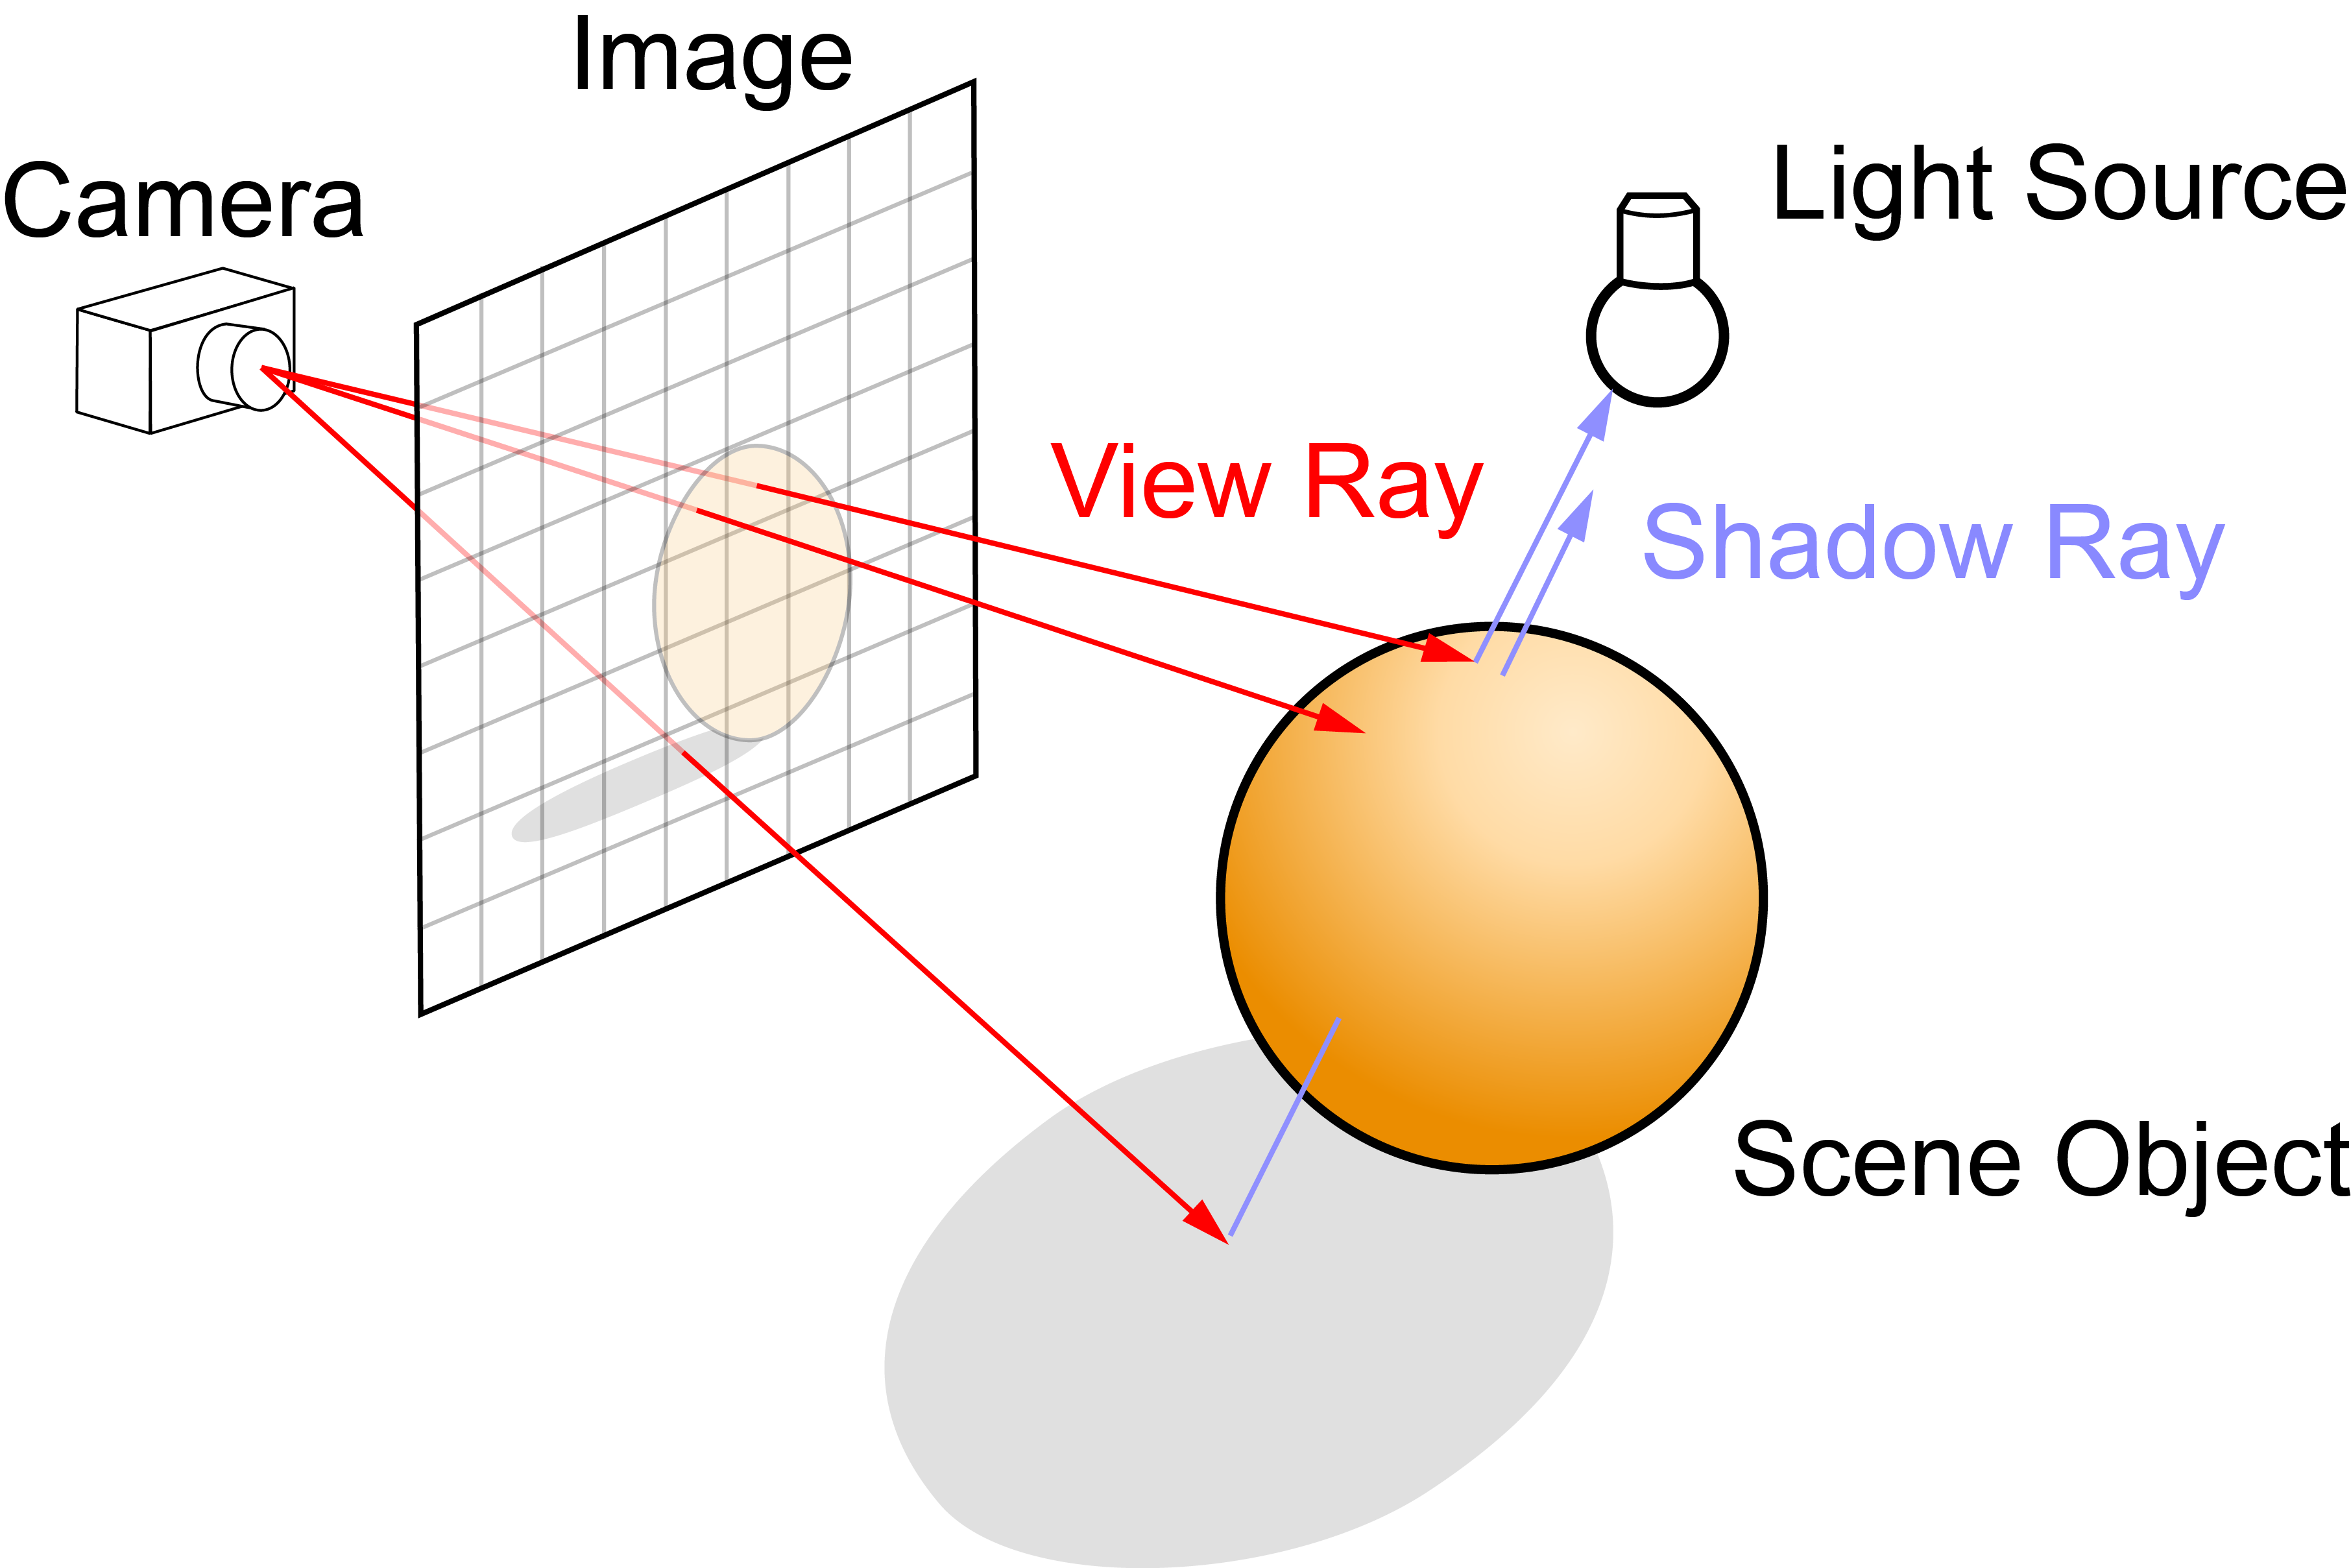
\includegraphics[width=0.8\textwidth,center]{raytrace.png}
\caption{Ilustración del funcionamiento de ray tracing.}
\end{figure}
\clearpage
Cada rayo se escribe $\textbf{r}(t)= o +td$ siendo $o$ el origen (el ojo) y $d$ la dirección entre el origen y el pixel que se desea calcular. Si tenemos la función implícita $F(p)=0$, donde $p \in {\rm I\!R} ^3 $, entonces para detectar la intersección de un rayo con una ecuación implícita basta con resolver $F(\textbf{r}(t))=0$.
\\A continuación a modo de ejemplo presentamos como obtener la intersección entre un rayo y una esfera de forma analítica\cite{realtimerendering}.
\\Sea la superficie implícita $F(p)=\lVert p -c \rVert - r = 0$, donde $c$ es el centro de la esfera y $r$ es el radio.
\begin{center}
$ F(\textbf{r}(t))= 0$
\\$ \leftrightarrow$
\\$ \lVert \textbf{r}(t) -c \rVert - r = 0$
\\$ \leftrightarrow$
\\$ \lVert \textbf{r}(t) -c \rVert = r$
\\ $\leftrightarrow$
\\ $(o+td -c).(o+td -c) = r^2 $ 
\\ $\leftrightarrow$
\\$t^2(d.d) + 2t(d.(o-c)) + (o-c).(o-c) - r^2=0$
\\ $\leftrightarrow$ \footnote{En este paso se asume que la el vector de dirección $d$ se encuentra normalizado}
\\$t^2 + 2t(d.(o-c)) + (o-c).(o-c) - r^2=0$
\end{center}
Utilizando báscara se obtienen los dos valores posibles de $t$ \footnote{Notar que si $d$ está normalizado $t$ es la distancia entre $o$ y el punto de intersección. $\lVert o + td - o \rVert = \lVert td\rVert = |t|\lVert d \rVert$}.
\\Para obtener un visualizador de ecuaciones implícitas el reto está en encontrar un método para hallar las raíces de la ecuación $F(r(t))=0$ para toda función implícita. El desafío es aún más complejo si se quiere lograr que éste funcione en tiempo real, ya que para cada frame se deberán realizar cientos de intersecciones entre rayos y la función.  
\subsubsection{Meshers}
Esta técnica consiste en obtener una aproximación poligonal de la geometría, para luego visualizarla utilizando cualquier método de visualización que soporte este tipo de geometría. Una vez realizada la aproximación poligonal ya no es necesario operar con la función para su visualización.
\\Para realizarla primero se obtiene una aproximación de la función realizando un muestreo de la misma. Una vez que se obtiene esto se aplica un algoritmo para la obtención de los polígonos (en la sección 3 se presentan 4).
\\La principal ventaja de este método sobre ray tracing es que una vez generada la aproximación no se debe trabajar más con la ecuación, esto permite que si se trabaja en tiempo real no ocurra que ecuaciones más complejas tengan framerates más bajos. Por este motivo este tipo de método es ideal para aplicaciones en tiempo real, ya que sólo se deben realizar operaciones complejas antes de iniciar la visualización, luego se puede visualizar utilizando por ejemplo la técnica del Z-buffer utilizando APIs como OpenGL o Direct3D.
\\La principal desventaja es que es una aproximación, por lo que si se utiliza ray tracing se obtendrá una imagen con un mayor nivel de similitud con respecto a la superficie.
\clearpage
\subsection{SURFER}
SURFER es una herramienta de Imaginary desarrollada en Java que permite la visualización de superficies implícitas del tipo algebraico. La misma utiliza JavaFX para la interfaz de usuario, y las ecuaciones se muestran utilizando el motor de render JSURFER, el cual es un raytracer implementado en CPU que utiliza el algoritmo de Descartes para hallar los puntos de intersección de los rayos con las ecuaciones. La aplicación utiliza proyección ortográfica para representar las ecuaciones en el plano.
\begin{figure}[h]
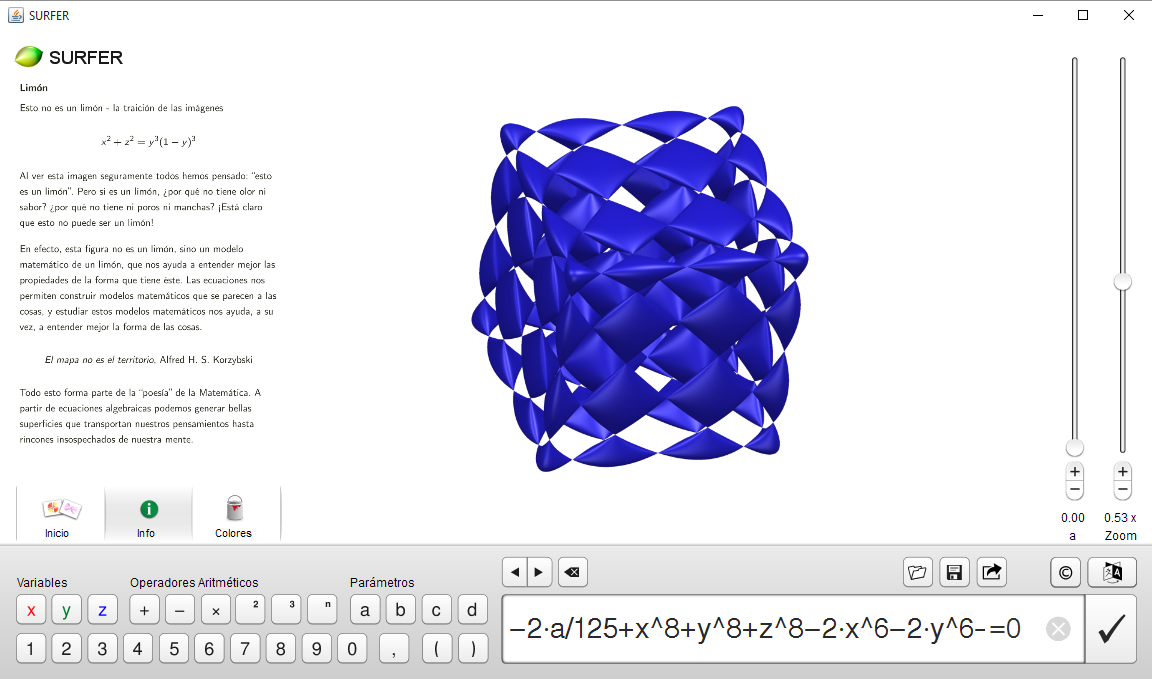
\includegraphics[width=\textwidth]{surfer_interfaz.png}
\caption{Interfaz del SURFER.}
\end{figure}
\\El programa cuenta con una interfaz amigable, a través de la cual es muy sencillo ingresar las ecuaciones. Para determinadas ecuaciones precargadas, cuenta con cierta información de modo de educar al usuario.
\\El motor utiliza el sombreado de Phong\cite{Phong} para la iluminación, por este motivo las figuras no proyectan sombras.
\\Al ser una aplicación que utiliza ray tracing la representación de las ecuaciones que se obtiene es muy fidedigna, pero para lograr funcionar en tiempo real muestra imágenes con una baja resolución mientras se está moviendo la cámara de forma de mantener 15 fps.
\\Hay que destacar que debido a que en cada frame la aplicación intersecta muchos rayos con la ecuación, la complejidad de la misma afecta la performance, es decir dependiendo de la ecuación la calidad de la imagen que se ve y el framerate que se obtiene. Esto se debe a que Surfer decide la resolución de la imagen a generar de forma dinámica dependiendo del tiempo que le lleva hacerla y de si la misma se está moviendo o no, de forma de no bajar demasiado de los 15 fps.
\begin{figure}[h]
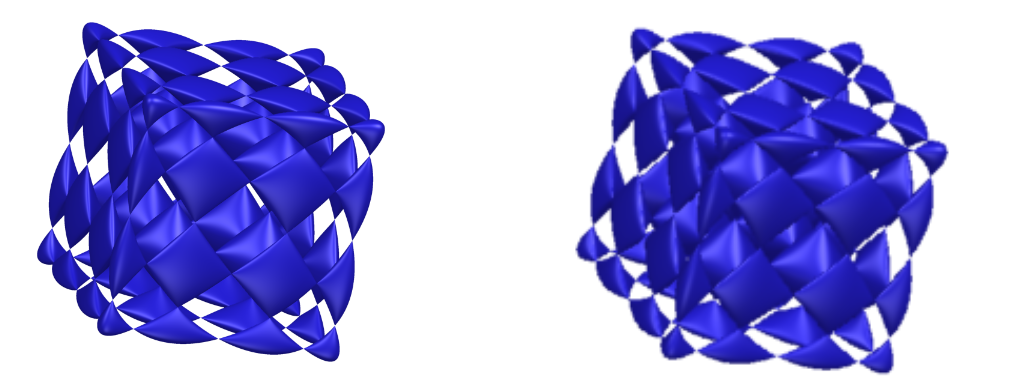
\includegraphics[width=\textwidth]{surfer_en_movimiento.png}
\caption{A la izquierda se ve la imagen una vez estabilizada, la cual posee una resolución de 796x796, mientras que a la derecha durante la rotación de la cámara la cual posee una resolución de 300x300.}
\end{figure}
\\En la imagen anterior se puede apreciar como baja la resolución de la ecuación cuando se rota la cámara de forma  que el framerate no sufra un impacto tan grande. Hay que destacar que cuanto más cerca de la pantalla se encuentre el observador se volverá aún más notorio el efecto de pixelación de la imagen producto de su baja resolución. También será muy notoria la inestabilidad en cuanto a la resolución, ya que cada vez que se rota la cámara la resolución baja de forma drástica. Considerando que es muy difícil que un  usuario de Oculus Rift o similar mantenga la cabeza lo suficientemente inmóvil de manera de que no baje la resolución, por lo que la mayoría del tiempo se estaría visualizando las superficies en baja resolución. El hecho de que la resolución de las imágenes es cercana a 300x300 probablemente provoque Virtual Reality Sickness\footnote{Este fenómeno se presenta en la sección 2.8}.
\\Se intentó extender esta aplicación para darle soporte al Oculus Rift. Persiguiendo este fin se realizaron una serie de pruebas, donde se detectó que la resolución de las imágenes es demasiado pequeña cuando se intenta generar dos imágenes (una desde el punto de vista de cada ojo) aunque fuesen ecuaciones sencillas. El efecto se puede apreciar en la imagen presentada a continuación donde en una versión modificada de SURFER se colocaron dos imágenes y a ambas se les aplicó la distorsión de barrido. La imagen de la izquierda es cuando están quietas, la de la derecha cuando hay movimiento\footnote{Para obtener estos valores se modificó el nivel al que intenta mantener el framerate SURFER, el cual fue disminuido a 12fps.}.
\begin{figure}[h]
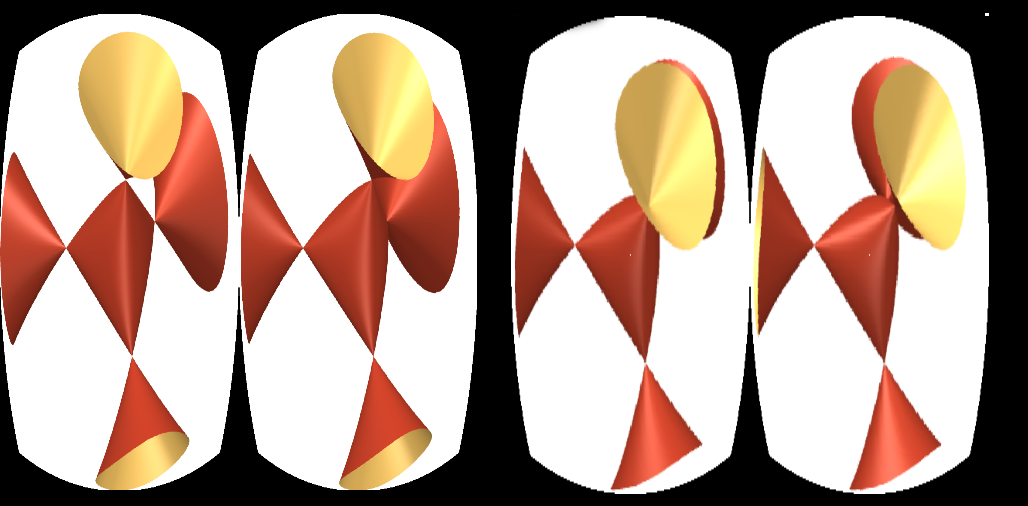
\includegraphics[width=\textwidth]{se_puede_doble.png}
\caption{A la izquierda se ve la imagen una vez estabilizada con una resolución de 796x796, mientras que a la derecha durante la rotación de la cámara con una resolución de 312x312.}
\end{figure}
\subsection{3d-XplroMath-J}
Otra aplicación que representa superficies es 3d-XplroMath-J, la cual es una reimplementación de 3d-XplroMath implementada en Java. Esta aplicación no usa ray tracing sino que utiliza aproximaciones poligonales. La aplicación fue inicialmente diseñada para utilizar JavaGraphics2D, pero luego se modificó para funcionar con OpenGL. 3D-XplorMath-J utiliza un  renderizador definido por una interfaz, Renderer3D, para extraer sus imágenes. 
\\OpenGL ofrece el dibujo 3D acelerados por hardware, con la posibilidad de gráficos mejorados y una gran aceleración en comparación con la aplicación de dibujo 3D con Graphics2D. OpenGL es implementado en Java utilizando la API JOGL.
\\Esta aplicación no cuenta con un ingreso de superficies de una forma tan amigable como SURFER. Las superficies se muestran de forma estática, y cuando se rota se muestra en modo wireframe.
\subsection{Isosurface}
	Isosurface es una aplicacion web que implementa los algoritmos de Marching cubes y Marching tetahedra en Javascript. La misma muestra algunas superficies de ejemplo, pero no permite introducir ecuaciones ni tiene menu interactivo que permita modificar las superficies mostradas . Ademas la aplicación muestra las superficies de una forma poligonal, resaltando los diferentes poligonos que se utilizan para aproximar la ecuación.  
\subsection{Visión estereoscópica}
Consiste en la percepción de la profundidad y la estructura de 3 dimensiones utilizando información derivada de los dos ojos. Debido a que los ojos de los seres humanos, se encuentran en diferentes posiciones laterales en la cabeza, los resultados de la visión binocular son dos imágenes ligeramente diferentes proyectados para las retinas de la los ojos. Las diferencias están principalmente en la posición horizontal relativa de los objetos en las dos imágenes. Estas diferencias posicionales se conocen como las disparidades horizontales o, más en general, la disparidades binoculares. Las disparidades se procesan en la corteza visual del cerebro para producir la percepción de profundidad. 
\begin{figure}[h!]
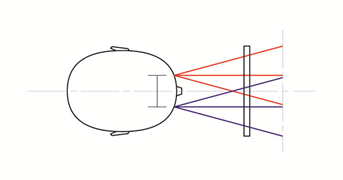
\includegraphics[width =0.7\linewidth, center]{ojos.png}
\caption{Disparidad binocular.}
\label{ fig : surface }
\end{figure}
\\Mientras que las disparidades binoculares están naturalmente presentes durante la visualización de una escena en 3 dimensiones real con dos ojos, las mismas deben ser simuladas mediante la presentación de dos imágenes diferentes por separado a cada ojo utilizando un método llamado estereoscópica. La percepción de la profundidad en tales casos también se refiere como "profundidad estereoscópica". 
\\La percepción de la profundidad y la estructura tridimensional  es, sin embargo, posible con la información de un ojo solamente, utilizando las diferencias en el tamaño de objeto y el paralaje de movimiento (diferencias en la imagen de un objeto a través del tiempo con el movimiento observador), aunque la impresión de profundidad en estos casos no es a menudo tan buena como la obtenida de las disparidades binoculares, por lo tanto, el término estereopsis (o profundidad estereoscópica) también puede referirse específicamente a la impresión única de profundidad asociada con la visión binocular, lo que coloquialmente se conoce como ver "en 3D".
\\La estereoscopía es una técnica para crear o mejorar la ilusión de profundidad en una imagen por medio de la estereopsis para la visión binocular. Cualquier imagen estereoscópica se llama un estereograma. 
\\La mayoría de los métodos estereoscópicas presentan  dos imágenes “movidas” por separado para el ojo izquierdo y derecho del espectador. Estas imágenes de dos dimensiones se combinan entonces en el cerebro para dar la percepción de la profundidad 3D.
\\Un fenómeno que puede acontecer es virtual reality sickness (también conocida como cybersickness y como simulator sickness), el cual se produce cuando la exposición a un entorno virtual causa síntomas que son similares a los síntomas de la motion sickness\cite{VRS} (en español el fenómeno es conocido como Cinetosis). Los síntomas más comunes son malestar general, dolor de cabeza, la conciencia del estómago, náuseas, vómitos, palidez, sudoración, fatiga, somnolencia, desorientación y apatía. Otros síntomas incluyen la inestabilidad postural y las arcadas. Este fenómeno tiende a caracterizarse por la desorientación.
\\Este efecto es diferente a la cinetosis, ya que puede ser causada por la percepción visual inducida de movimiento. No es necesaria que la persona se mueva para sufrir sus síntomas.
\\La fisiología de la VRS actualmente no está claramente entendido. Afortunadamente, la investigación ha descubierto algunas indicaciones claras de ciertas condiciones que la causan. Parece que las imágenes proyectadas desde la realidad virtual tienen un gran impacto en la enfermedad. La frecuencia de actualización de las imágenes en pantalla a menudo no es lo suficientemente alta cuando se produce la VRS. Debido a que la frecuencia de actualización es más lenta que los procesos cerebrales, causa una descoordinación entre el tipo de procesamiento y la velocidad de actualización, lo que hace que el usuario perciba fallos en la pantalla. Cuando estos dos componentes no coinciden, puede causar al usuario las mismas sensaciones que cuando se experimenta motion sickness.
\\La resolución sobre la animación también puede hacer que los usuarios experimentan este fenómeno\cite{oculussickness}. Cuando animaciones son pobres, que es causa de otro tipo de discordia entre lo que se espera y lo que realmente está sucediendo en la pantalla. Cuando los gráficos en pantalla no mantienen el ritmo con movimientos de la cabeza del usuario, puede desencadenar una forma de la motion sickness.
\subsection{Tecnologías existentes para visión estereoscópica}
En la actualidad está saliendo al mercado una gran serie de dispositivos que aplican los conceptos de la estereoscopía para generar el efecto de estar en un espacio virtual.
\\Existen varios productos para dispositivos no móviles, por ejemplo  Oculus Rift\cite{oculus}, Playstation VR\cite{psvr} y HTC Vive\cite{htcvive}. A su vez existen varios para dispositivos móviles como  Google Cardboard\cite{cardboard} y  Samsung Gear VR\cite{samsungvr}, estos dispositivos requieren de celulares para funcionar (utilizándolos como pantalla y como sensor de rotación).
\\Estos dispositivos tienen en común es que cuentan con una pantalla, dos cristales y sensores para reconocer los movimientos de la cabeza \footnote{Particularmente rotaciones, aunque actualmente algunos de ellos utilizan cámaras de forma de poder reconocer si se mueve la cabeza hacia adelante o hacia atrás por medio del traqueo de una luz}.
\\La resolución de las pantallas, así como su velocidad de refresco varían según el dispositivo. Este es un aspecto muy importante, ya que la calidad final de la experiencia se verá muy afectada por este factor, debido a que si la imagen se encuentra muy pixelada la experiencia no será agradable, y si la velocidad de refresco no es buena se podrá producir mareos y nauseas al usuario.
\\Los sensores son utilizados principalmente para permitir al usuario mirar hacia “los costados” de forma de explorar la escena, generando un mayor nivel de inmersión.
\\Los cristales de los dispositivos de visión estereoscópica proveen un campo visual (FOV) muy amplio, permitiendo una mayor inmersión, pero para lograrlo generan una distorsión\cite{oculusrendering} en la imagen como muestra la siguiente figura. 
\\Este tipo de distorsión se conoce como  distorsión de acerico (pincushion distortion en inglés), lo que provocaría que si no se utiliza ningún tipo de corrección sobre las imágenes que se le envían al dispositivo, todo se vería distorsionado como se ve en la imagen.
\begin{figure}[h!]
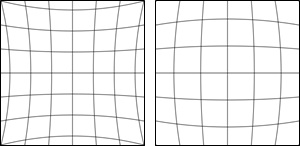
\includegraphics[width =0.6\linewidth, center]{ace-bar.png}
\caption{ A la izquierda se puede apreciar la distorsión de acerico y a la derecha la de barril.}
\label{ fig : surface }
\end{figure}
\\Para corregir la deformación producida se utiliza la distorsión de barril (barrel distortion en inglés), la cual genera el efecto inverso (como se puede ver en la imagen) y provoca que el usuario que utiliza los lentes no se de cuenta de la curvatura de los cristales, pero siendo beneficiado por la inmersión generada por el gran campo visual. 
\\A continuación mostramos una imagen “clásica” en las tres formas, la primera es como se ve normalmente, la del medio es si se le aplica una distorsión de barrido y la última es como se visualiza luego de una distorsión de acerico.
\begin{figure}[h!]
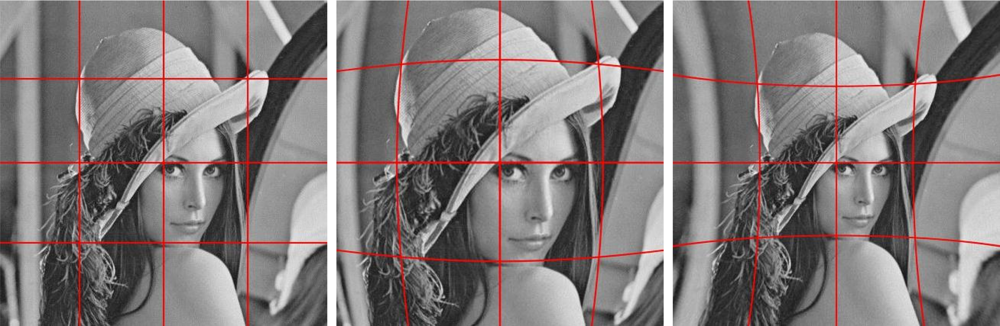
\includegraphics[width=0.8\textwidth, center]{imagen_clasica.png}
\caption{Se muestra la imagen sin distorsionar y luego de aplicar cada una de las distorsiones mencionadas.}
\end{figure}
\clearpage
\subsubsection{ Oculus Rift}
El Oculus Rift es un casco de realidad virtual desarrollado y fabricado por Oculus VR, lanzado al mercado el 28 de marzo de 2016. Antes del lanzamiento de la versión para el consumidor se lanzaron varias para los desarrolladores, a continuación se presentan algunas de ellas.
\paragraph{Development kit 1}
La versión DK1 (Development Kit 1) utiliza una pantalla de 7 pulgadas (18 cm) con un tiempo de refresco de píxeles significativamente menor que el prototipo original, lo que reduce la latencia y el motion blur al girar la cabeza rápidamente. El “relleno de píxeles” también fue mejorado, lo que  implica que el usuario no nota con tanta facilidad los píxeles en pantalla. El LCD es más brillante y la profundidad de color es de 24 bits por píxel. La pantalla tiene una resolución de 1280x800 (en total, no por ojo) y posee una velocidad de refresco de 60Hz.
\begin{figure}[h!]
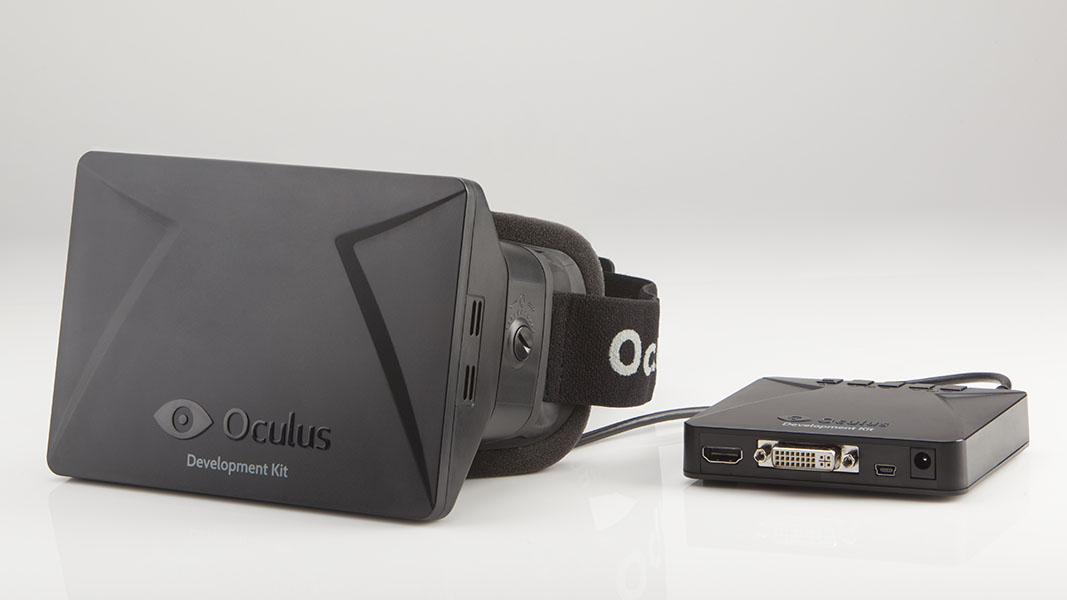
\includegraphics[width=0.8\textwidth,center]{dk1.jpg}
\caption{Oculus Rift Development Kit 1.}
\end{figure}
\\Esta versión cuenta con una pequeña “caja de control” donde se conecta lo necesario, y para su funcionamiento además de ser conectado a la computadora por medio de un cable USB y un cable de video (por ejemplo HDMI), debe ser conectado a la corriente.
\paragraph{Development kit 2}
Oculus comenzó a distribuir a los clientes que habían reservado DK2 ( Development Kit 2) en julio de 2014. Esta nueva versión ofrece varias mejoras clave en relación al primer kit de desarrollo, tales como tener una mayor resolución (960x1080 por ojo, es decir 1920x1080 en total, la resolución que se conoce como FullHD), una pantalla OLED, una mayor frecuencia de refresco de 75 Hz, el seguimiento de posición a través de un sensor externo al Rift, un cable desmontable,  la omisión de la necesidad de la caja de control externa y finalmente ya no es más necesario conectarlo a la corriente.
\begin{figure}[h!]
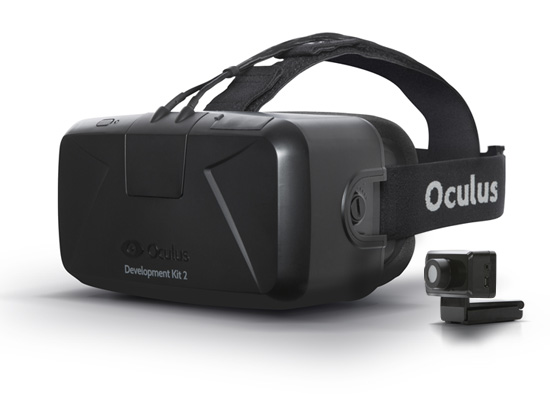
\includegraphics[width=0.8\textwidth,center]{dk2.jpg}
\caption{Oculus Rift Development Kit 2.}
\end{figure}
\\La pantalla pasó de ser de 7 a 5.7 pulgadas. Una exploración del dispositivo, reveló que incorpora un smartphone Samsung Galaxy Note 3 modificado como pantalla.
\paragraph{Consumer version}
La versión que fue lanzada para el público en general tiene una pantalla OLED de 1080x1200 por ojo, una tasa de refresco de 90 Hz y 110 $^{\circ}$ campo de visión. Posee auriculares integrados que proporcionan un sonido con efecto 3D, efecto de rotación y de seguimiento de posición. El sistema de seguimiento de posición, denominada "Constellation", se realiza mediante un sensor IR LED USB que se encuentra apuntando hacia el dispositivo Rift, que normalmente se encuentra en el escritorio del usuario, e identifica toda la habitación con luces infrarrojas y LED, lo que crea un espacio 3D, permitiendo al usuario utilizar el dispositivo mientras se está sentado, de pie o caminar alrededor de la misma habitación. 
\begin{figure}[h!]
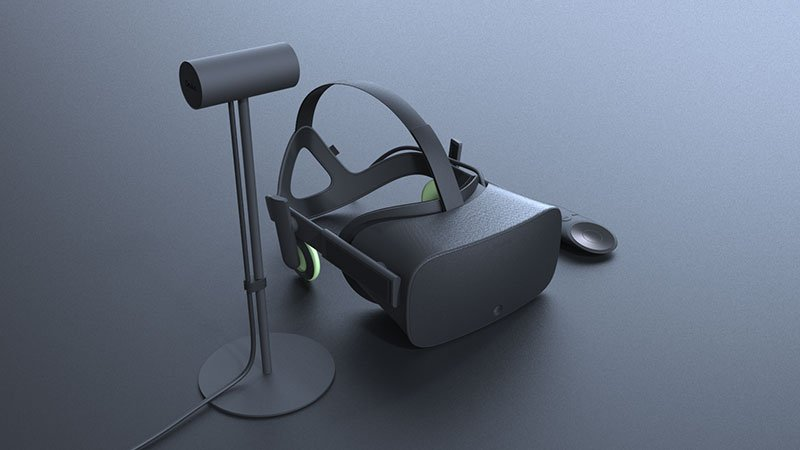
\includegraphics[width=0.8\textwidth,center]{cv.jpg}
\caption{Oculus Rift Consumer Version.}
\end{figure}
\begin{table}[h!]
  \centering
  \label{tab:table1}
  \begin{tabular}{cccc}
    \toprule
     & DK1 & DK2 & CV\\
    \midrule
    OLED & No & Sí & Sí\\
    Resolución & 1280x800 & 1920x1080 & 2160x1200 \\
    Frecuencia de refresco de imagen & 60Hz & 75Hz & 90Hz\\
    Campo Visual & 110 grados & 100 grados & 110 grados\\
    Acelerómetro, giroscopio, magnetómetro & Sí & Sí & Sí\\  
    Frecuencia de refresco del acelerómetro & 1000Hz& 1000Hz & 1000Hz\\
    Traqueo orientacional & Sí & Sí & Sí\\ 
    Traqueo posicional & No & Sí & Sí\\
    Caja de control externa & Sí & No & No\\
    \bottomrule
  \end{tabular}
  \caption{Comparación entre las versiones de Oculus Rift.}
\end{table}
\clearpage
\subsubsection{HTC Vive}
Este dispositivo posee una resolución de 2160 x 1200, un campo visual de 110 grados y una tasa de refresco de 90 Hz. Este dispositivo es comercializado con dos controles que rastrean el movimiento de las manos para poder brindar experiencias más inmersivas\cite{htcvive}.
\begin{figure}[h!]
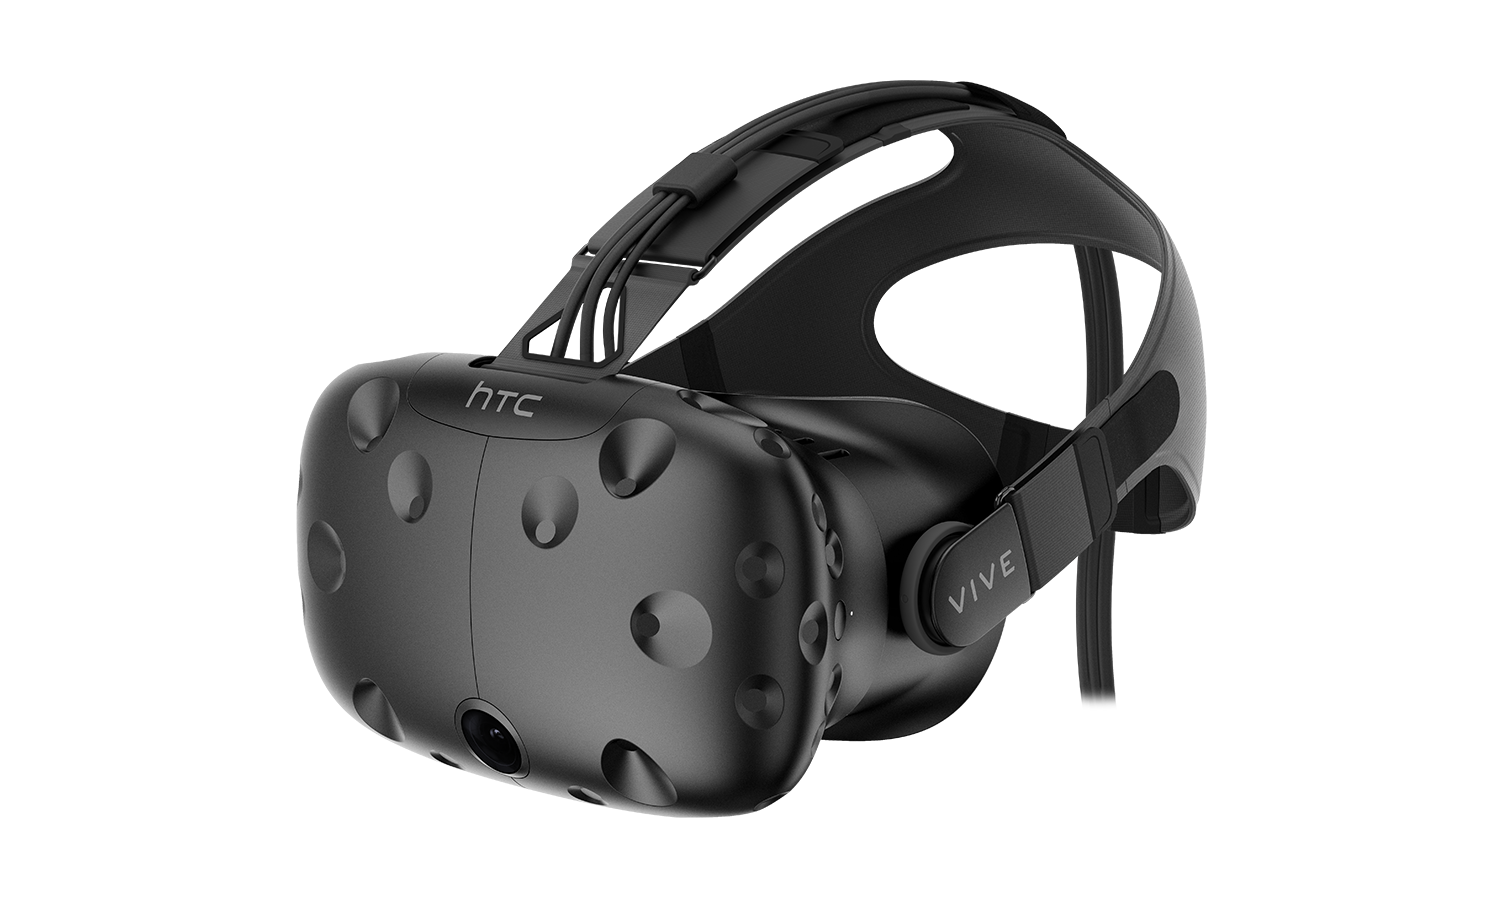
\includegraphics[width=0.8\textwidth,center]{htc.png}
\caption{HTC Vive.}
\end{figure}
\subsubsection{PlaystationVR}
Es el dispositivo para la visión estereoscópica de Sony para ser utilizado con su consola de videojuegos PlaySation 4. A diferencia de los otros equipos, no ha sido lanzada al mercado, se prevee que sea lanzado en octubre del presente año. Por más que no este disponible, la empresa anunció que no será compatible con PC.
\\Posee una pantalla de 5,7 pulgadas, y una resolución de 1920x1080, es decir 960x1080 por ojo. La velocidad de refresco es de 90 Hz o 120 Hz y tiene un campo visual de 100 grados\cite{psvrspecs}.
\clearpage
\begin{figure}[h!]
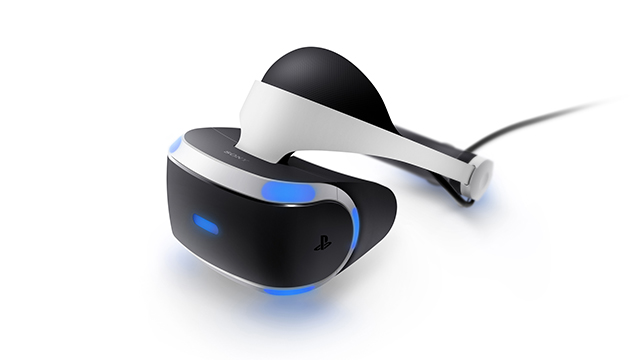
\includegraphics[width=0.8\textwidth,center]{psvr.jpg}
\caption{PlaystationVR.}
\end{figure}
\subsubsection{Google Cardboard}
Es una plataforma de realidad virtual desarrollada por Google\cite{cardboard} para su uso con un visor plegable y teléfono inteligente. Llamado así por su visor de cartón plegable, pretende ser un sistema de bajo costo para estimular el interés y el desarrollo de aplicaciones de realidad virtual. Los usuarios pueden construir su propio visor de componentes simples y de bajo coste utilizando las especificaciones publicado por Google, o comprar una de las versiones pre-fabricadas. Para utilizarlo es necesario  la colocación de un dispositivo móvil en la parte posterior de la carcasa y se  visualiza a través de los lentes en la parte delantera.
\begin{figure}[h!]
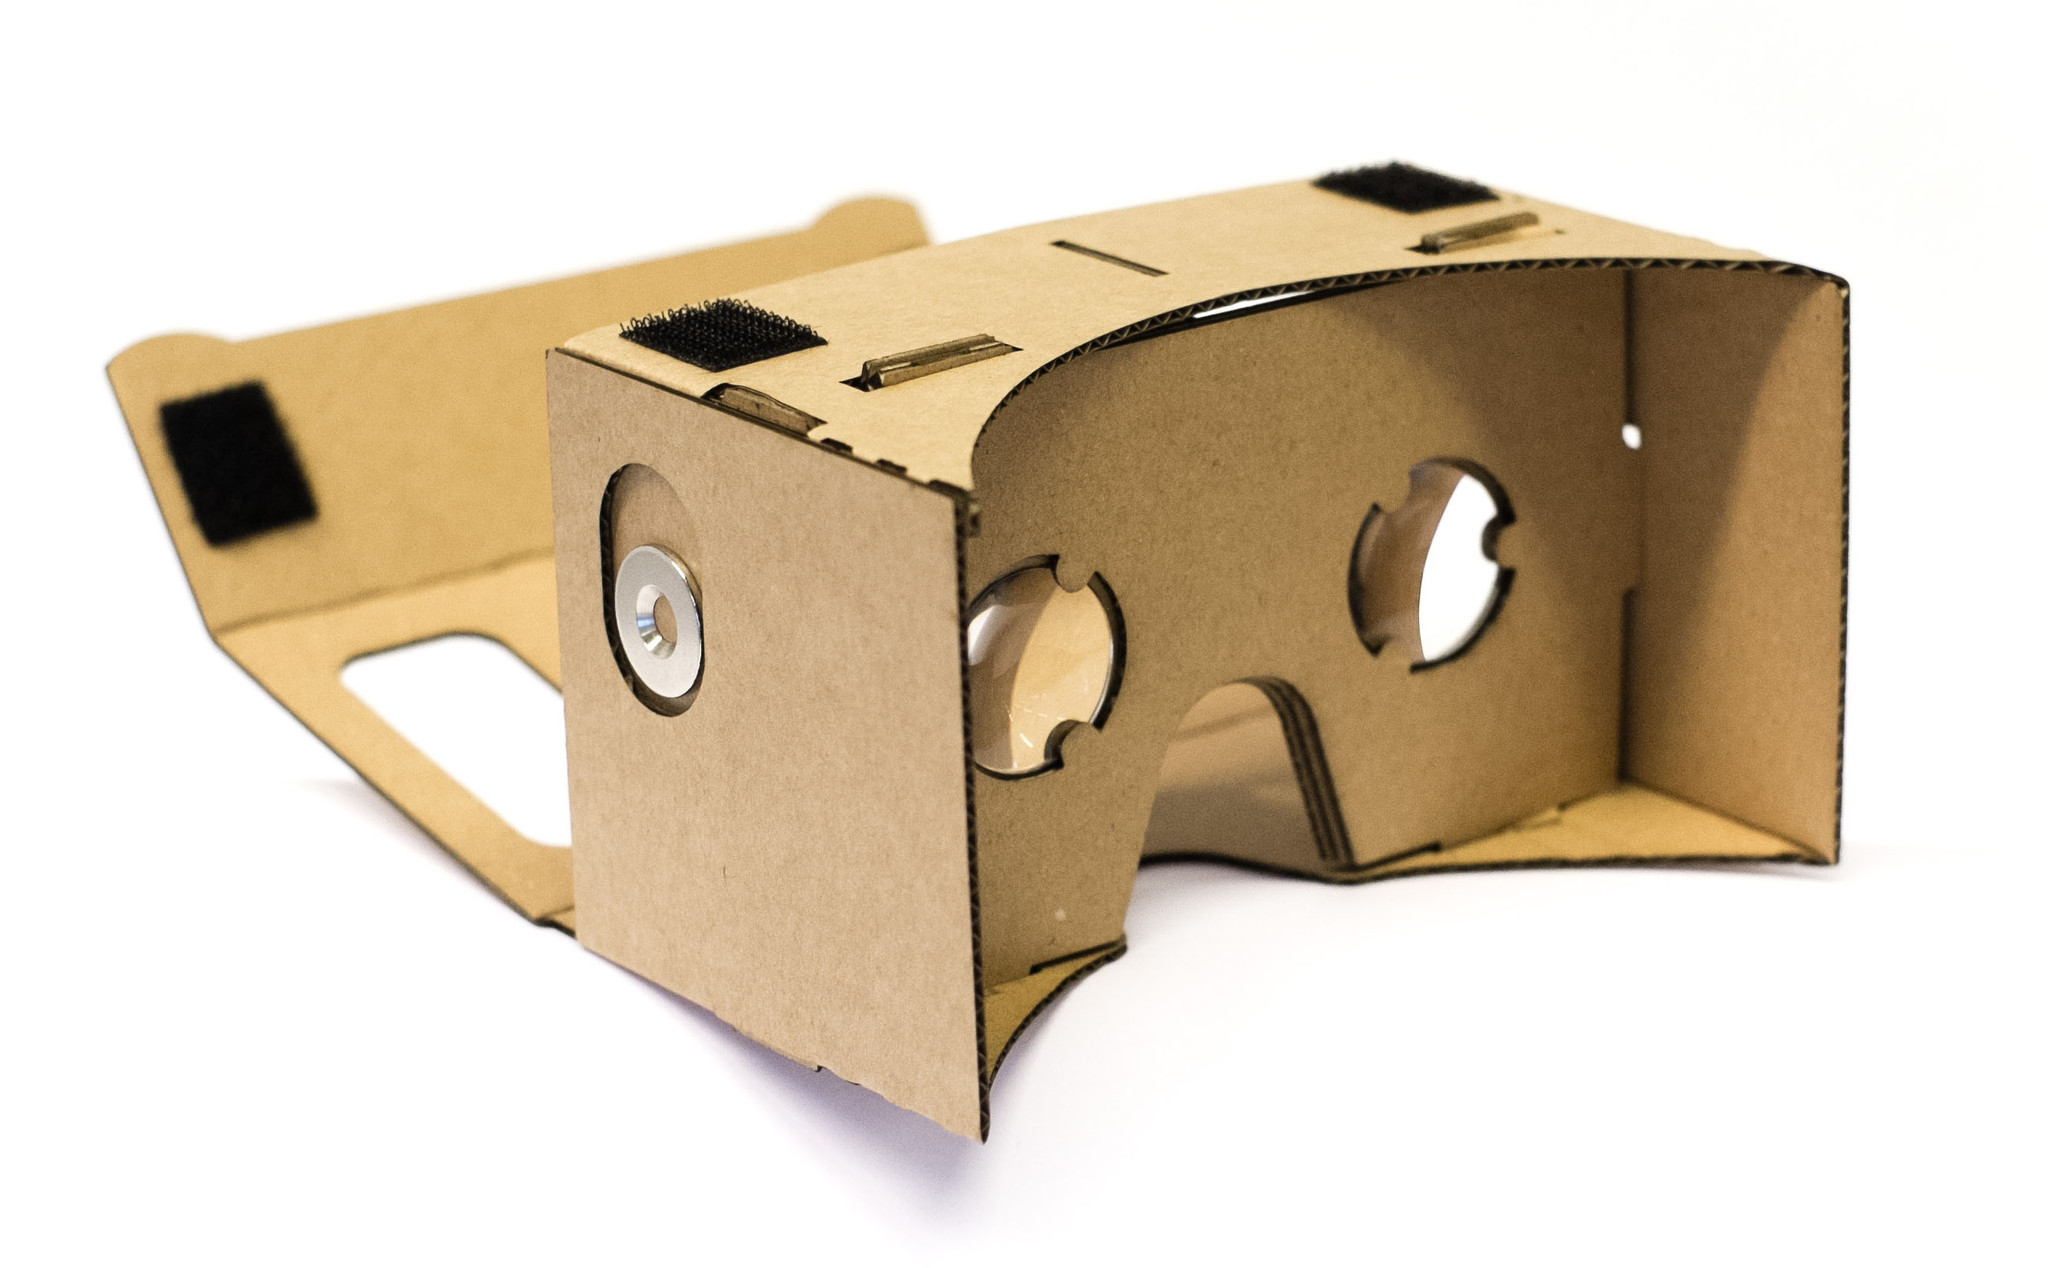
\includegraphics[width=0.7\textwidth,center]{google_cardboard.jpg}
\caption{Ejemplo de Google Cardboard.}
\end{figure}
\\Fue introducido en la Google I/O 2014, donde un visualizador Google Cardboard fue regalado a todos los asistentes. El kit de desarrollo (SDK) está disponible para los sistemas operativos Android e iOS, mientras que una separada VR Ver SDK permite a los desarrolladores integrar contenidos de RV en la web, así como en sus aplicaciones móviles. 
\subsubsection{Samsung Gear VR}
Al igual que Google Cardboard, requiere un celular para su funcionamiento. En este caso el teléfono debe ser un Samsung Galaxy S6, Samsung Galaxy Note5 o Samsung Galaxy S7\cite{samsungvr}. Lo que lo hace más restrictivo que Google Cardboard.
\\Este dispositivo fue desarrollado en conjunto con Oculus\cite{samsungvr}.
\begin{figure}[h!]
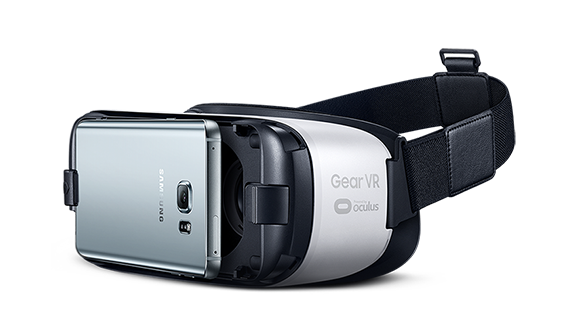
\includegraphics[width=0.8\textwidth,center]{samsungvr.png}
\caption{Samsung Gear VR.}
\end{figure}
\clearpage
\subsection{Software Gráfico}
\subsubsection{WebGL}
WebGL (Web Graphics Library) es una API de JavaScript para la representación  de gráficos 3D y 2D  interactivos dentro de cualquier navegador web compatible sin el uso de plug-ins. WebGL está integrado en la mayoría de los navegadores que permiten acelerado por la GPU, el uso de la física y de procesamiento de imágenes. Los elementos de WebGL se pueden mezclar con otros elementos HTML y componerse con otras partes de la página. Los programas que utilizan WebGL tienen código escrito en JavaScript y  código de sombreado que se ejecuta en la unidad de procesamiento gráfico de un ordenador (GPU). 
\subsubsection{THREEJS}

THREEJS es una biblioteca liviana\cite{three} de JavaScript para trabajar con 3D, puede ser utilizado con un canvas de HTML5 o con WebGL. Fue creada en 2010, aunque originalmente fue desarrollada en ActionScript, pero rápidamente fue traducida a JavaScript\footnote{El código fuente se puede obtener en \cite{codigothree}}.
\\Posee como característica principal que es compatible con todos los navegadores compatibles con WebGL, esto permite que las aplicaciones desarrolladas con él sean posibles de ejecutar en la gran mayoría de los navegadores modernos.
\\Además la biblioteca permite utilizar WebGL de forma más sencilla y accesible, ya que trae ciertas funcionalidades ya implementadas.
\subsubsection{MozVR}
Es el proyecto de Mozilla para agregar la posibilidad de usar realidad virtual en páginas web (WebVR)\cite{mozvr}. Permite que versiones experimentales de Firefox sean compatibles con Oculus Rift (Firefox Nightly\cite{nightly}).
\\Esto permite utilizar el WebGL para generar páginas web que sean experimentadas en realidad virtual de forma eficiente.
\subsubsection{GLSL}
OpenGL Shading Language (GLSL) es un lenguaje de programación de shaders de alto nivel el cual está basado en C. Fue creado por la OpenGL ARB ( OpenGL Architecture Review Board) para dar a los desarrolladores un control más directo del pipeline gráfico sin tener que utilizar ARB assembly o lenguajes específicos de hardware .
\\Con este lenguaje se pueden desarrollar tanto vertex shaders como pixel shaders (fragment shaders). Ambos tipos se ejecutan en la tarjeta de video. Los vertex shaders se ejecutan en la etapa de geometría del pipeline gráfico, se ejecuta una vez por cada vértice, permitiendo cambiar la posición generando desplazamientos, con el fin de lograr efectos interesantes. Los pixels o fragment shaders se ejecutan una vez por cada pixel.

\clearpage
\section{Aproximación de superficies algebraicas}
Para la generación de superficies algebraicas existen diversas formas. En rasgos generales se pueden distinguir estos algoritmos en 2 categorías: Los que funcionan mediante la intersección de rayos contra la superficie( Raytracing), y aquellos que generan una aproximación lineal mediante polígonos (Meshers).
\\En el proyecto se ha decidido utilizar los algoritmos que caen en la categoría de Meshers\cite{mykola1}\cite{mykola2} a pesar de que sólo aproximan la superficie, debido a que tienen un tiempo de respuesta menor a la hora de realizar movimientos (rotación y traslación), lo cual es indispensable a la hora de evitar la Virtual Reality Sickness luego de la renderización de la superficie en el Oculus Rift.
\\Existen diversos algoritmos que caen en la categoría de Meshers y realizan una aproximación por polígonos de las superficies o volúmenes de las ecuaciones. Se presentan a continuación una serie de conceptos matemáticos sobre los cuales se basan los algoritmos que se presentan más adelante.
\begin{figure}[h]
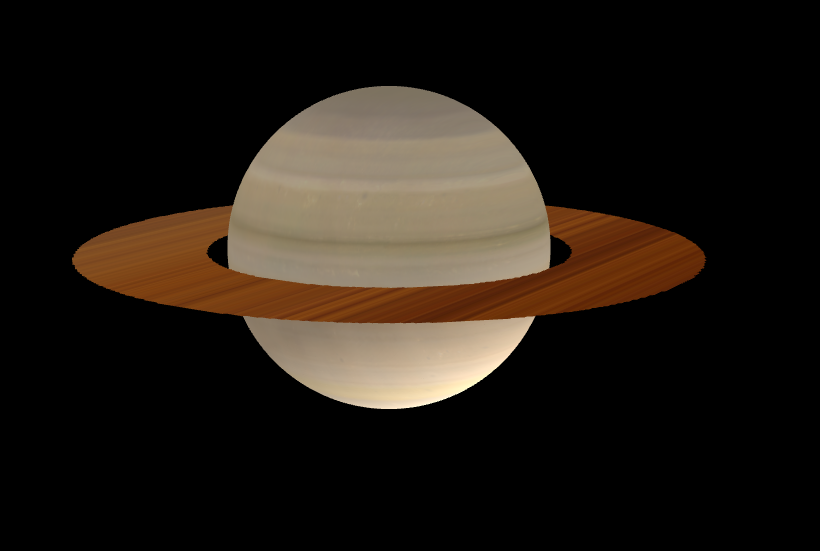
\includegraphics[width=\textwidth]{saturno.png}
\caption{Ejemplo de utilización de meshers para generar una esfera y un disco. Se puede notar en el disco que la aproximación no es exacta, ya que se notan ciertos problemas de aliasing.}
\end{figure}
\clearpage
\subsection{Conjuntos de nivel}
Son un conjunto de puntos en los que se iguala una función a una constante, es decir:
$Lc(f) = {(x1,...,xn) | f(x1,...,xn)  = c}$

Ejemplos de conjuntos de nivel:
\begin{figure}[h!]
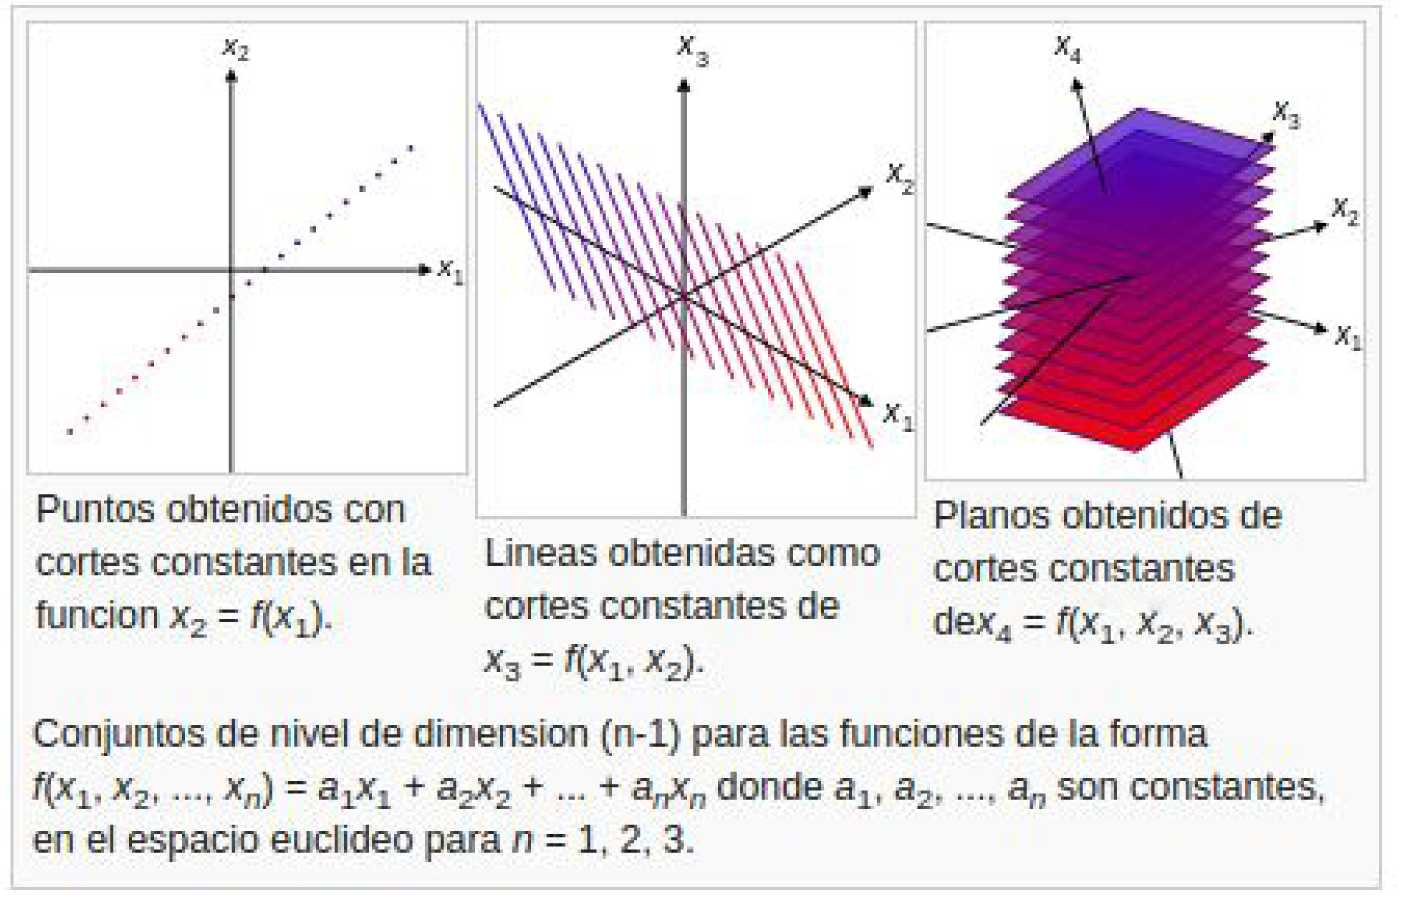
\includegraphics[width=0.73\textwidth,center]{meshers1.png}
\caption{Ejemplos de distintos tipos de conjuntos de nivel de funciones lineales.}
\end{figure}
\begin{figure}[h!]
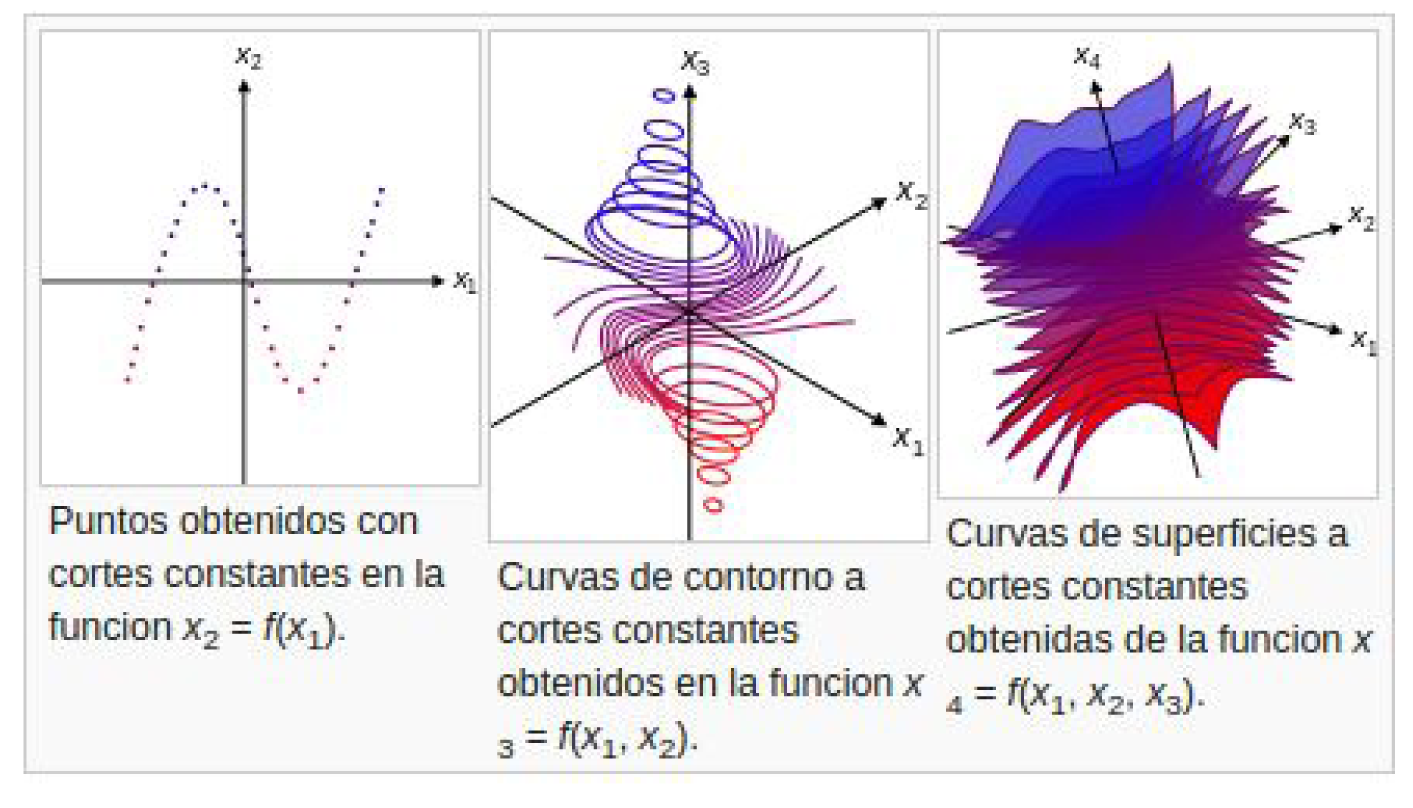
\includegraphics[width=0.73\textwidth,center]{meshers2.png}
\caption{Ejemplos de distintos tipos de conjuntos de nivel de funciones no lineales.}
\end{figure}
\clearpage
\subsection{Teorema de la función implícita}
En algunas ecuaciones es sencillo convertir una función del tipo $f(x,y,z)  = z- x^2 - y^2$ en una ecuación paramétrica: 
$x(u,v) = u$
$y(u,v) = v$
$z(u,v) = u^2+v^2$
\\Este tipo de funciones es trivial de dibujar (basta con tomar diferentes valores de $u$ y $v$ y formar polígonos con las coordenadas obtenidas de los mismos).
Pero lamentablemente no todas las funciones se pueden parametrizar, y por lo tanto no todas son igualmente de sencillas de dibujar, es por eso que existen los siguientes algoritmos.
\subsection{Interpolación trilinear}
La interpolación trilinear\cite{inter} es un método de interpolación en una grilla regular 3-dimensional. Se aproxima al valor de un punto intermedio $(x, y, z)$ en el eje local del prisma rectangular en forma lineal, a partir de datos en los puntos de la grilla. Para realizar la interpolación trilinear se necesitan 8 puntos adyacentes.
Considere un cubo de largo una unidad con el vértice inferior-izquierdo como origen como se muestra en la siguiente figura.
\begin{figure}[h!]
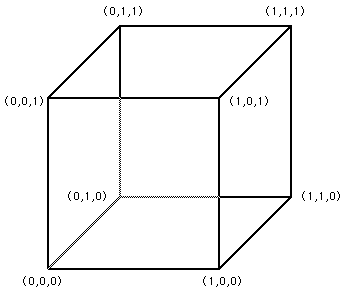
\includegraphics[width=0.65\textwidth,center]{inter.png}
\caption{Caja utilizada en la iterpolación trilinear. Los valores de cada vértice se denotarán por $V_{000}$,$V_{001}$,$V_{010}$,...,$V_{111}$.}
\end{figure}
\\El valor en la posición $(x,y,z)$ dentro del cubo se denotará por $V_{xyz}$ y esta definida como
\begin{center}
$V_{xyz}=V_{000}(1-x)(1-y)(1-z) + V_{100}x(1-y)(1-z) + V_{010}(1-x)y(1-z) + V_{001}(1-x)(1-y)z + V_{101}x(1-y)z + V_{011}(1-x)yz + V_{110}xy(1-z) + V_{111}xyz$
\end{center}
Supongamos que tenemos una aproximación de f mediante el muestreo en una grilla cúbica en una resolución fija. Para obtener los valores intermedios necesitamos tan solo realizar una interpolación trilineal entre los puntos de la grilla.


\subsection{Marching Cubes}
El algoritmo de Marching cubes\cite{marching}\cite{marchingcubes} consiste en la creación de superficies mediante la intersección de las aristas de una grilla tridimensional con el volumen de la superficie misma. Donde la superficie intersecta una arista de la grilla, el algoritmo crea un vértice. Mediante la utilización de una tabla de diferentes triángulos dependiendo de los diferentes patrones de intersección con la arista, el algoritmo crea una superficie.
\\El problema fundamental es formar una aproximación de una superficie a través de un campo escalar dentro de una grilla rectangular 3D. Dada una celda (cubo de la grilla), definida por sus vértices y los valores escalares en cada vértice, es necesario crear caras planas que mejor representan la superficie dentro de ese cubo de la cuadrícula. La superficie puede, o no, pasar a través del cubo de la cuadrícula, y cortar cualquiera de los vértices. Cada posibilidad de corte con el cubo de la grilla se caracteriza por el número de vértices en que la celda tiene valores por encima o por debajo de la superficie. Si un vértice está por encima de la superficie y un vértice adyacente está por debajo de la superficie, entonces sabemos que la superficie corta el borde entre estos dos vértices. La posición en la que corta el borde será interpolada linealmente, y la relación de longitud entre los dos vértices será la misma que la relación de la superficie a los valores de los vértices del cubo de la cuadrícula.
\\Por convención se indexara los vértices y aristas del cubo de la grilla de la siguiente forma:
\begin{figure}[h!]
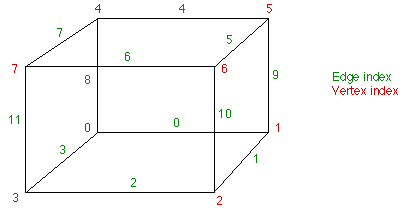
\includegraphics[width=0.75\textwidth,center]{marchingcubes1.png}
\caption{Cubo con la indexación utilizada en el algoritmo de Marching Cubes.}
\end{figure}
\\Si por ejemplo el valor en el vértice 3 está por debajo del valor superficie y todos los valores en todos los demás vértices están por encima del valor superficie, entonces se crea una cara triangular que corta a través de las aristas 2,3 y 11. La posición exacta de los vértices de la cara triangular depende de la relación del valor superficie a los valores en los vértices 3-2, 3-0, 3-7, respectivamente.
\begin{figure}[h!]
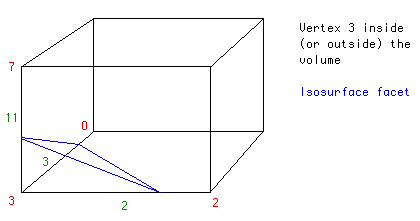
\includegraphics[width=0.75\textwidth,center]{marchingcubes2.png}
\caption{Ejemplo de creación de una cara en una celda con Marching Cubes.}
\end{figure}
Lo que hace al algoritmo "difícil" es el gran número de combinaciones posibles (256) y la necesidad de obtener una combinación de caras consistente para cada solución de forma que las caras generadas en las celdas adyacentes se conecten entre sí correctamente.\\
La primera parte del algoritmo utiliza una tabla (edgeTable) que mapea los vértices bajo la superficie a los bordes de intersección. Se forma un índice de 8 bits donde cada bit corresponde a un vértice.
\lstset{language=C}          % Set your language (you can change the language for each code-block optionally)

\begin{lstlisting}[frame=single][caption=blabla, label=amb]
   cubeindex = 0;
   if (grid.val[0] < isolevel) cubeindex |= 1;
   if (grid.val[1] < isolevel) cubeindex |= 2;
   if (grid.val[2] < isolevel) cubeindex |= 4;
   if (grid.val[3] < isolevel) cubeindex |= 8;
   if (grid.val[4] < isolevel) cubeindex |= 16;
   if (grid.val[5] < isolevel) cubeindex |= 32;
   if (grid.val[6] < isolevel) cubeindex |= 64;
   if (grid.val[7] < isolevel) cubeindex |= 128;
\end{lstlisting}

La búsqueda en la tabla devuelve un número de 12 bits, cada bit corresponde a una arista, 0 si la arista no se corta por la superficie, 1 si la arista se corta por la superficie. Si ninguno de las aristas retorna un corte en la tabla, se devuelve un 0, esto ocurre cuando cubeindex es 0 (todos los vértices por debajo de la superficie) o 0xff (todos los vértices por encima de la superficie).
Utilizando el ejemplo anterior donde sólo el vértice 3 estuvo por debajo de la superficie, cubeindex sería igual a 0000, 1000 o 8. edgeTable [8] = 1000 0000 1100. Esto significa que el borde 2,3, y 11 son intersectados por la superficie.
Los puntos de intersección se calculan ahora por interpolación lineal. Si P1 y P2 son los vértices de una arista de corte y V1 y V2 son los valores escalares en cada vértice, el punto de intersección P está dada por:
P = P1 + (isovalue - V1) (P2 - P1) / (V2 - V1)
\begin{figure}[h!]
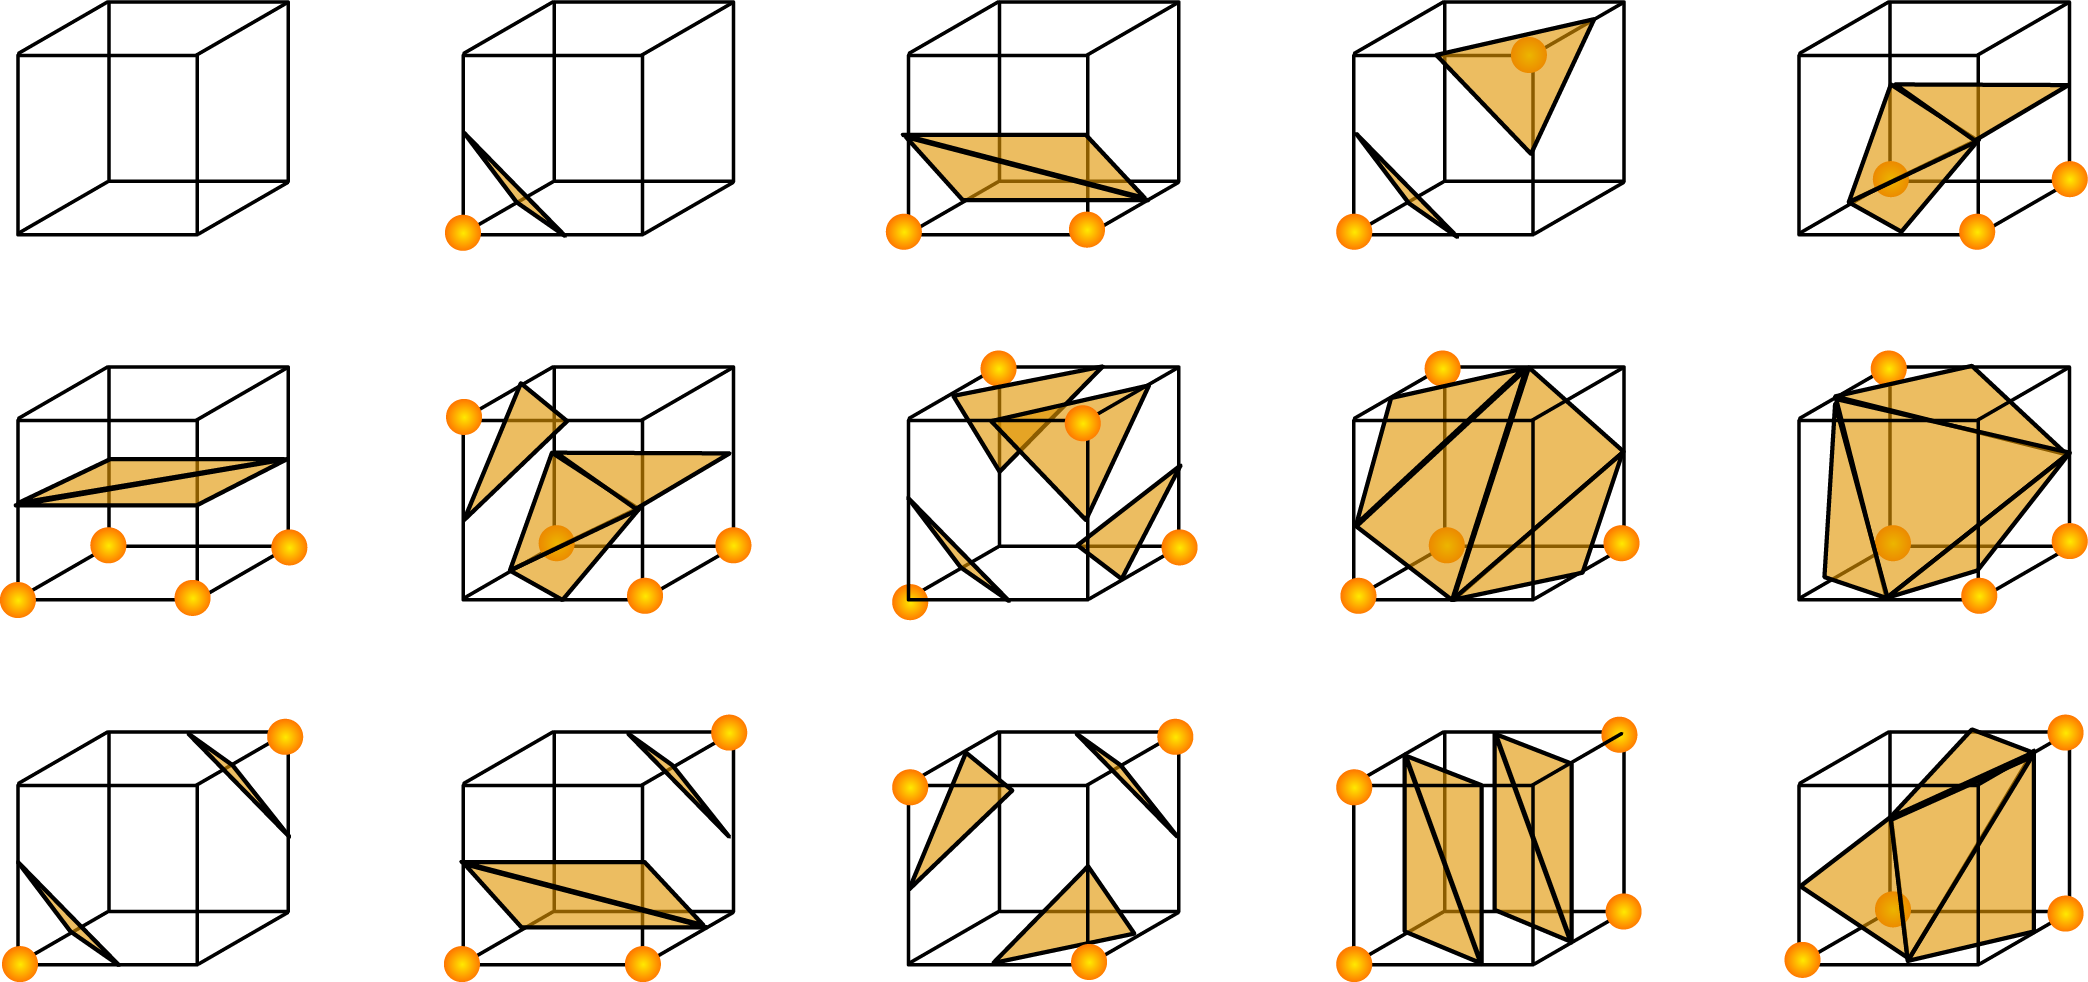
\includegraphics[width=0.8\textwidth,center]{marchingcubes3.png}
\caption{Ejemplos de formación de caras dentro de una celda.}
\end{figure}
\\La última parte del algoritmo implica la formación de las caras correctas en las posiciones en que la superficie intersecta los bordes del cubo de la grilla. La tabla triTable utiliza el cubeindex como entrada y retorna las aristas de la grilla que  formarán parte de los vértices de las caras triangulares que sean necesarias para representar la superficie dentro del cubo de la grilla. Hay como máximo 5 caras triangulares en un cubo de la grilla.
Volviendo a nuestro ejemplo, en el paso anterior se calculan los puntos de intersección a lo largo del borde 2,3 y 11. El octavo elemento en la triTable es:
{3, 11, 2, -1, -1, -1, -1, -1, -1, -1, -1, -1, -1, -1, -1, -1},
\\Este es un ejemplo particularmente simple, pero las combinaciones que pueden surgir no son tan evidentes para muchos de los casos de la tabla.
\\Otro ejemplo.
\\Digamos que el vértice 0 y 3 están por debajo del superficie. Entonces cubeindex será 0000 1001 == 9. La novena entrada en la egdeTable es 905hex == 1001 0000 0101 lo que significa que las aristas 11,8,2 y 0 se cortan, por lo que trabajamos los vértices de la intersección de la superficie con esos bordes.
A continuación, 9 en la triTable es 0, 11, 2, 8, 11, 0. Esto corresponde a 2 caras triangulares, una entre la intersección del borde de 0 11 y 2. La otra entre las intersecciones a lo largo de los bordes 8 11 y 0.
\subsubsection{Resolución de la grilla}
Algo deseable a controlar cuando se poligoniza una superficie es la resolución de la cuadrícula de muestreo. Esto permite elegir el grado de la aproximación a la superficie a generarse en función de la suavidad requerida y / o la potencia de procesamiento disponible para mostrar la superficie. El siguiente ejemplo ilustra una misma superficie generada a diferentes tamaños de malla:
\clearpage
\begin{figure}[h!]
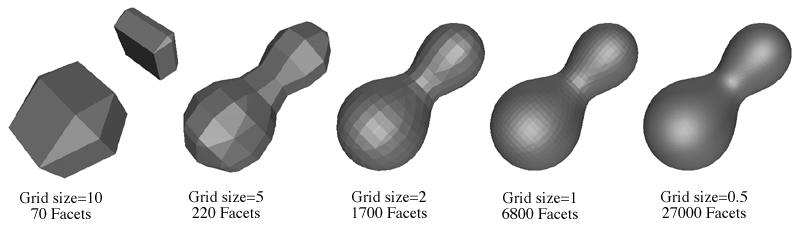
\includegraphics[width=0.8\textwidth,center]{marchingcubes4.png}
\caption{Ejemplo de la misma figura utilizando diferentes tamaños de grilla, se puede notar que en la primer figura, debido a que el tamaño de celda elegido es grande, no genera una figura correctamente.}
\end{figure}
\subsubsection{Determinación de las normales de los vértices de las caras triangulares}
A menudo es necesario crear las normales para cada vértice de las caras triangulares para poder representar una superficie “suave”. Una forma de hacer esto es ,después de que las caras han sido creadas, promediar las normales de todas las caras que comparten un vértice del triángulo. A continuación se muestra el resultado suave a la derecha, la imagen de la izquierda tiene la única normal para la faceta aplicada a cada uno de los vértices. El modelo a continuación es de un tipo particular de neurona capturado de un microscopio confocal.\\
\begin{figure}[h]
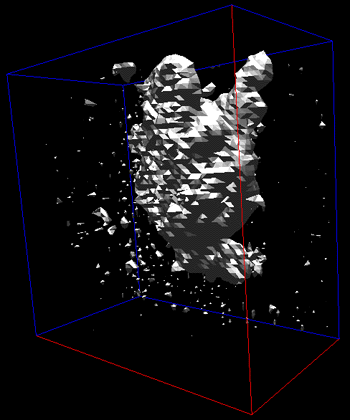
\includegraphics[width =0.45\linewidth]{marchingcubes5.png}
\hfill
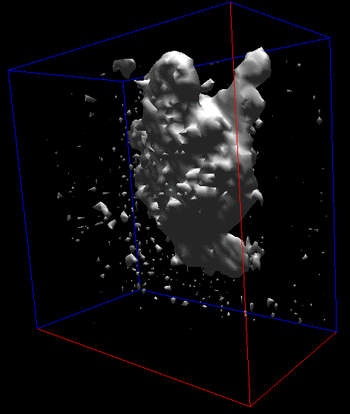
\includegraphics[width =0.45\linewidth]{marchingcubes6.png}
\caption{ Ejemplos de distintas configuraciones de normales de la misma figura.}
\label{ fig : surface }
\end{figure}
\\Un enfoque común es asignar a cada vértice una media ponderada de las normales de los polígonos que comparten el vértice. El peso es la inversamente proporcional al área del polígono, por lo que pequeños polígonos tienen mayor peso. La idea es que los pequeños polígonos pueden ocurrir en las regiones de alta curvatura de la superficie.
\subsection{Marching Tetrahedra}
El algoritmo Marching Tetrahedra\cite{marching}\cite{marchingt} muestrea el espacio en los vértices de una malla 3D rectangular. Cada celda de la malla se divide en 6 tetraedros .Hay que tener en cuenta que las aristas del tetraedro se alinean con los de las celdas de caja adyacentes, y existe un método de dividir la caja en 5 tetraedros que no tiene esta propiedad.
\\La aproximación de las caras se calcula para cada tetraedro de forma independiente. Los vértices de la cara son determinados por interpolación lineal dónde la superficie corta las aristas del tetraedro.
\begin{figure}[h!]
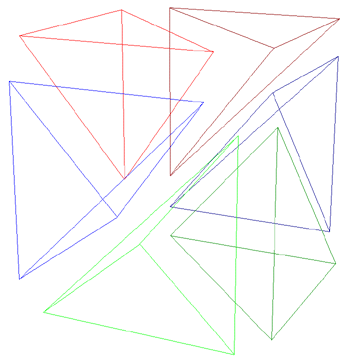
\includegraphics[width=0.6\textwidth,center]{mt1.png}
\caption{Ejemplo de división de una grilla 3d rectangular en 6 tetrahedros.}
\end{figure}
\clearpage
Hay 8 casos diferentes. Los círculos huecos y rellenos en los vértices del tetraedro indican que los vértices están en diferentes lados de la superficie, al costado de cada ejemplo se puede ver la codificación binaria utilizada para identificar el correspondiente caso. Los casos no ilustrados se dan cuando todos los vértices están por encima o por debajo de la superficie, no se generan caras en esos 2 últimos casos.\\
\begin{figure}[h!]
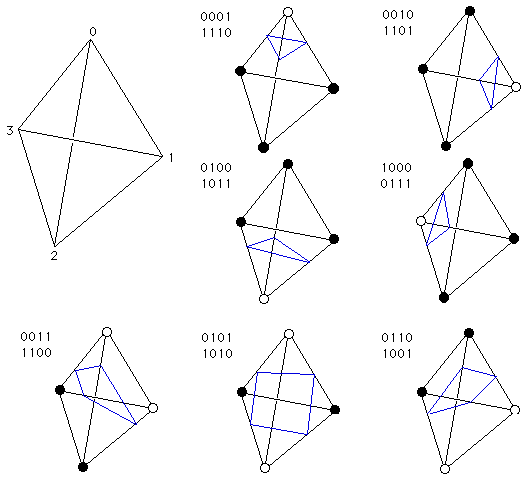
\includegraphics[width=0.7\textwidth,center]{mt2.png}
\caption{Ejemplos de generación de caras en el tetrahedro.}
\end{figure}\\
\textbf{Notas}
\begin{itemize}
\item Esta técnica no sufre de las ambigüedades a diferencia del algoritmo anterior.
\item Dado que se trata de un muestreo discreto, es posible que se pierda parte de la superficie si varía dentro de una celda de la caja. Aunque éste es un problema estándar en cualquier conjunto de datos muestreados de forma discreta.
\item Si la orientación de las caras es importante (horario o antihorario), entonces los pares de los casos que se tratan de la misma manera anteriormente necesitan ser tratados por separado. Las caras para cada par tienen que tener ambas los mismos vértices, pero se deben ordenar de una manera que dependa de si el "interior" del objeto que se poligoniza tiene valores altos o bajos.
\end{itemize}

\subsection{Surface Nets}
La idea de Surface Nets es dividir el espacio en cubos, luego a cada cubo, a los que llamaremos celdas, se le aplica una operación en cada uno de sus 8 vértices de forma de determinar si se encuentra dentro de la figura o no. Si los 8 vértices tienen el mismo valor ese cubo no se dibuja. En otro caso se dibuja. Esta es la versión más simple. La imagen que se presenta a continuación a la izquierda utiliza ese método.
\begin{figure}[h]
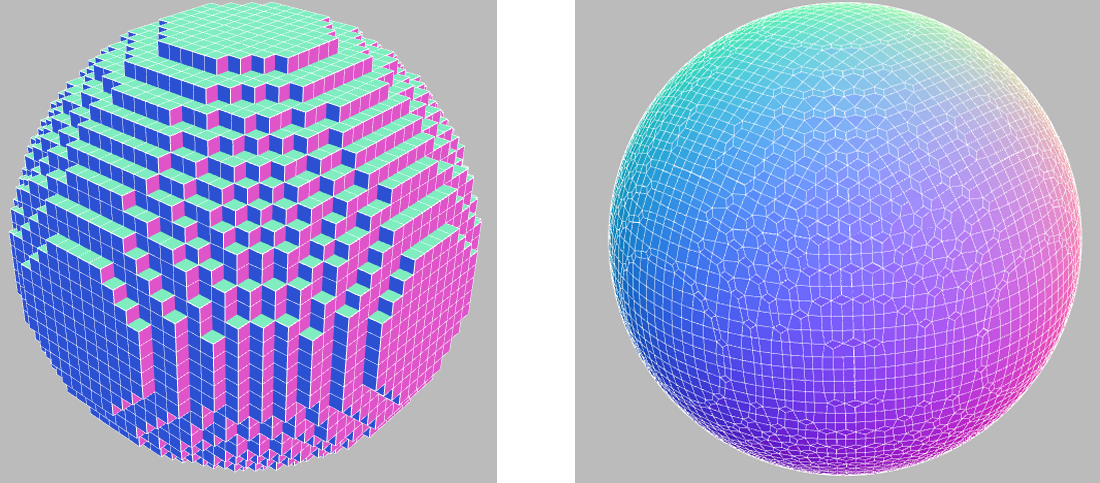
\includegraphics[width =\linewidth,center]{snc.png}
\caption{ A la izquierda se puede apreciar una aproximación de una esfera sin suavizado, mientras que a la derecha la superficie se encuentra la misma superficie con suavizado.}
\label{ fig : surface }
\end{figure}
\\La idea del original del algoritmo Surface Nets\cite{surfacenets}, tiene una forma de “suavizar” las superficies. Utiliza una serie de operaciones de forma de evitar que la malla que genera se vea “dura”.
\\Para lograrlo se pueden utilizar distintas técnicas de selección de los vértices, la selección de las técnicas es vital para la performance así como para la calidad de las mallas. El paper original de Gibson[20]  propone utilizar una estrategia de minimización de la energía global y aplicarle ecuaciones de suavizado. Para hacerlo se parte de un vértice elegido al azar (en el paper original el centro del cubo)  y se perturba (usando la técnica de descenso por el gradiente) hasta que llegue en algún momento a la superficie. Esta técnica es muy buena teóricamente, pero tiene ciertos inconvenientes de performance, ya que hay que hallar una gran cantidad de mínimos. Esto provoca (particularmente en javascript) que demore demasiado.
\\La idea de Naive Surface Nets (el método que está disponible en la aplicación, el cual fue propuesto por Mykola Lysenko\cite{mykola1}\cite{mykola2}) es elegir el vértice de forma más simple  en lugar de encontrar el vértice óptimo, se computan las intersecciones con las aristas de las celdas (como en Marching cubes) y luego se toma su centro de masa como el vértice en cada cubo (o celda). La malla que se obtiene de este proceso es similar a la de Marching Cubes, sólo que con un menor número de vértices y caras. 
\\Elegir el vértice de esta forma permite hacer el algoritmo mucho más rápido, aunque se pierde calidad.
\subsection{Dual Contouring}
Este algoritmo es una extensión del algoritmo de Marching cubes y Surface Nets. Mantiene un vértice en el centro del cubo de la grilla, pero añade la generación de superficies a través de octrees, para poder dibujar más precisamente aquellas superficies “ásperas”. \\A diferencia de los 3 algoritmos presentados anteriormente este no está disponible en la aplicación desarrollada. Aún así nos pareció importante mencionarlo\cite{dualcontour}.
\clearpage
\section{Alcance del proyecto}
A continuación se plantean los objetivos específicos que se consideraron a la hora de desarrollar la aplicación final. A su vez se presentan una serie de decisiones de diseño importantes que fueron tomadas a lo largo del proyecto, así como la justificación pertinente asociada.
\subsection{Objetivos}
El principal objetivo del proyecto es lograr visualizar ecuaciones utilizando Oculus Rift y que la experiencia del usuario en dicho dispositivo fuera agradable. Por ese motivo el framerate de la aplicación es importante, ya que este debe poder mantenerse como mínimo por encima de los $60 fps$ generando dos puntos de vista distintos al mismo tiempo para reducir la probabilidad de VRS. Ademas, como objetivos secundarios se requeria: poder explorar la ecuación de manera interactiva, pudiendo navegar por ella libremente, visualizar no solo superficies algebraicas como el surfer sino tambien ecuaciones implícitas en general, ingresar las ecuaciones en un lenguaje simple, similar al de otras herramientas matematicas como MATLAB y Derive.
\\Con la intención de hacer la aplicación lo más atractiva posible se plantearon varios objetivos en cuanto a la visualización de las superficies. Entre estos objetivos se encuentran la capacidad de aplicarle texturas a las superficies, aplicarle luces dinámicas a la escena que puedan ser modificadas por el usuario en tiempo real, la presencia de sombras y la utilización de algunos shaders que generen efectos visualmente atractivos sobre las superficies.
\\Persiguiendo atraer al público más joven, así como una mayor comodidad de los usuarios se puso como objetivo la compatibilidad con joystick.
\\Al utilizar meshers se planteó como objetivo el poder proveer a los usuarios una interfaz para poder de alguna forma almacenar las geometrías generadas, de forma de no tener que recalcularlas en caso de querer visualizarlas nuevamente.
\\También se trazó como objetivo el tener los menúes de la aplicación en varios idiomas, de manera de hacer la aplicación accesible al mayor número de personas posible.
\\Considerando que los meshers generan una aproximación de la superficie en una zona especifica, se decidió proveer a los usuarios de una forma visual y simple de elegir qué zona se desea generar.
\\Finalmente la capacidad de no visualizar una única ecuación a la vez, es decir contar con una modalidad alternativa donde se permita la visualización de varias ecuaciones al mismo tiempo.
\subsection{Decisiones de diseño}
La principal decisión que se tomó fue no utilizar raytracing y utilizar meshers. Esta decisión se efectuó considerando los framerates y la resolución de las imágenes obtenidos utilizando raytracing, los cuales eran inferiores a lo recomendado para una buena experiencia estereoscópica. Por ese motivo se optó por tomar como base Isosurface en lugar de SURFER. Para la toma de esta decisión también fue considerado el hecho de que de esta forma la aplicación podría generar ecuaciones implícitas, mientras que SURFER genera solo ecuaciones algebraicas. Esto permite una visualización de una cantidad mayor de superficies, aunque como se mencionó anteriormente tiene el costo de que se visualiza una aproximación, por lo que la calidad de la ecuación se ve afectada. Considerando la ganancia en performance, así como en cantidad de superficies que se pueden presentar, luego de varias pruebas se decidió que la perdida de calidad generada por la aproximación era aceptable.
\\Se decidió utilizar dos patrones de diseño utilizados generalmente en videojuegos estos son el \textit{Update Patten} y el \textit{Game Loop Pattern}\cite{patterns}\cite{engine}. El \textit{Update Patten} consiste en delegar a los diferentes elementos de la escena su actualización en la etapa previa al renderizado del frame. Esto se efectúa en la etapa de Update o Animate, en esta etapa todos los elementos de la escena se modifican en caso de ser necesario para representar el estado actual. El \textit{Game Loop Pattern} consiste en contar con un loop principal, el cual es el encargado de realizar las etapas previas y renderizar los frames. Existen varias variantes del mismo\cite{patterns}, donde se utilizan distintos criterios sobre la forma de controlar el tiempo que ha transcurrido desde el frame anterior. Se decidió utilizar la versión que utiliza una variable y almacena el tiempo en milisegundos que ha transcurrido. Al decidirse que se realizaría una aplicación web, la aplicación del patrón no es la más directa, ya que a diferencia de lo que sucede en otro tipo de plataformas la aplicación queda embebida dentro del loop del navegador. Por este motivo para utilizar este patrón se debe llamar a $requestAnimationFrame$\cite{patterns}.
\begin{figure}[h]
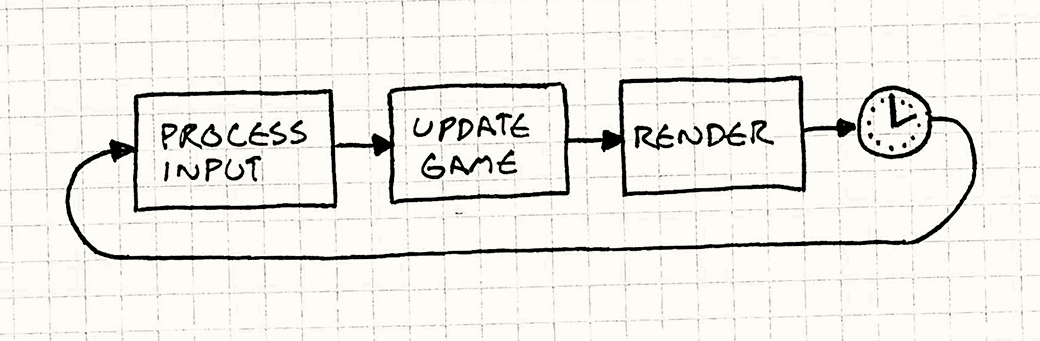
\includegraphics[width =0.7\linewidth, center]{gameloop.png}
\caption{Estructura del patrón \textit{Game Loop Pattern}\cite{patterns}.}
\label{ fig : surface }
\end{figure}
\\También se optó por utilizar una arquitectura Model-View-Controller (MVC). Modularizando los distintos componentes, para obtener asi una aplicacion mas mantenible, y facil de entender, ademas de ser una arquitectura estandar en muchas aplicaciones web. Por eso, se separo el modelo, es decir, la parte de generación de los puntos y planos de la figura (por ejemplo el MarchingCubes.js, SurfaceNets.js, junto al service.js etc), de la parte que se comunica con la interfaz del usuario (controller.js), además la vista se encuentra hecha en los archivos index.html y los diversos archivos dentro de la carpeta css.
\clearpage
\begin{figure}[h!]
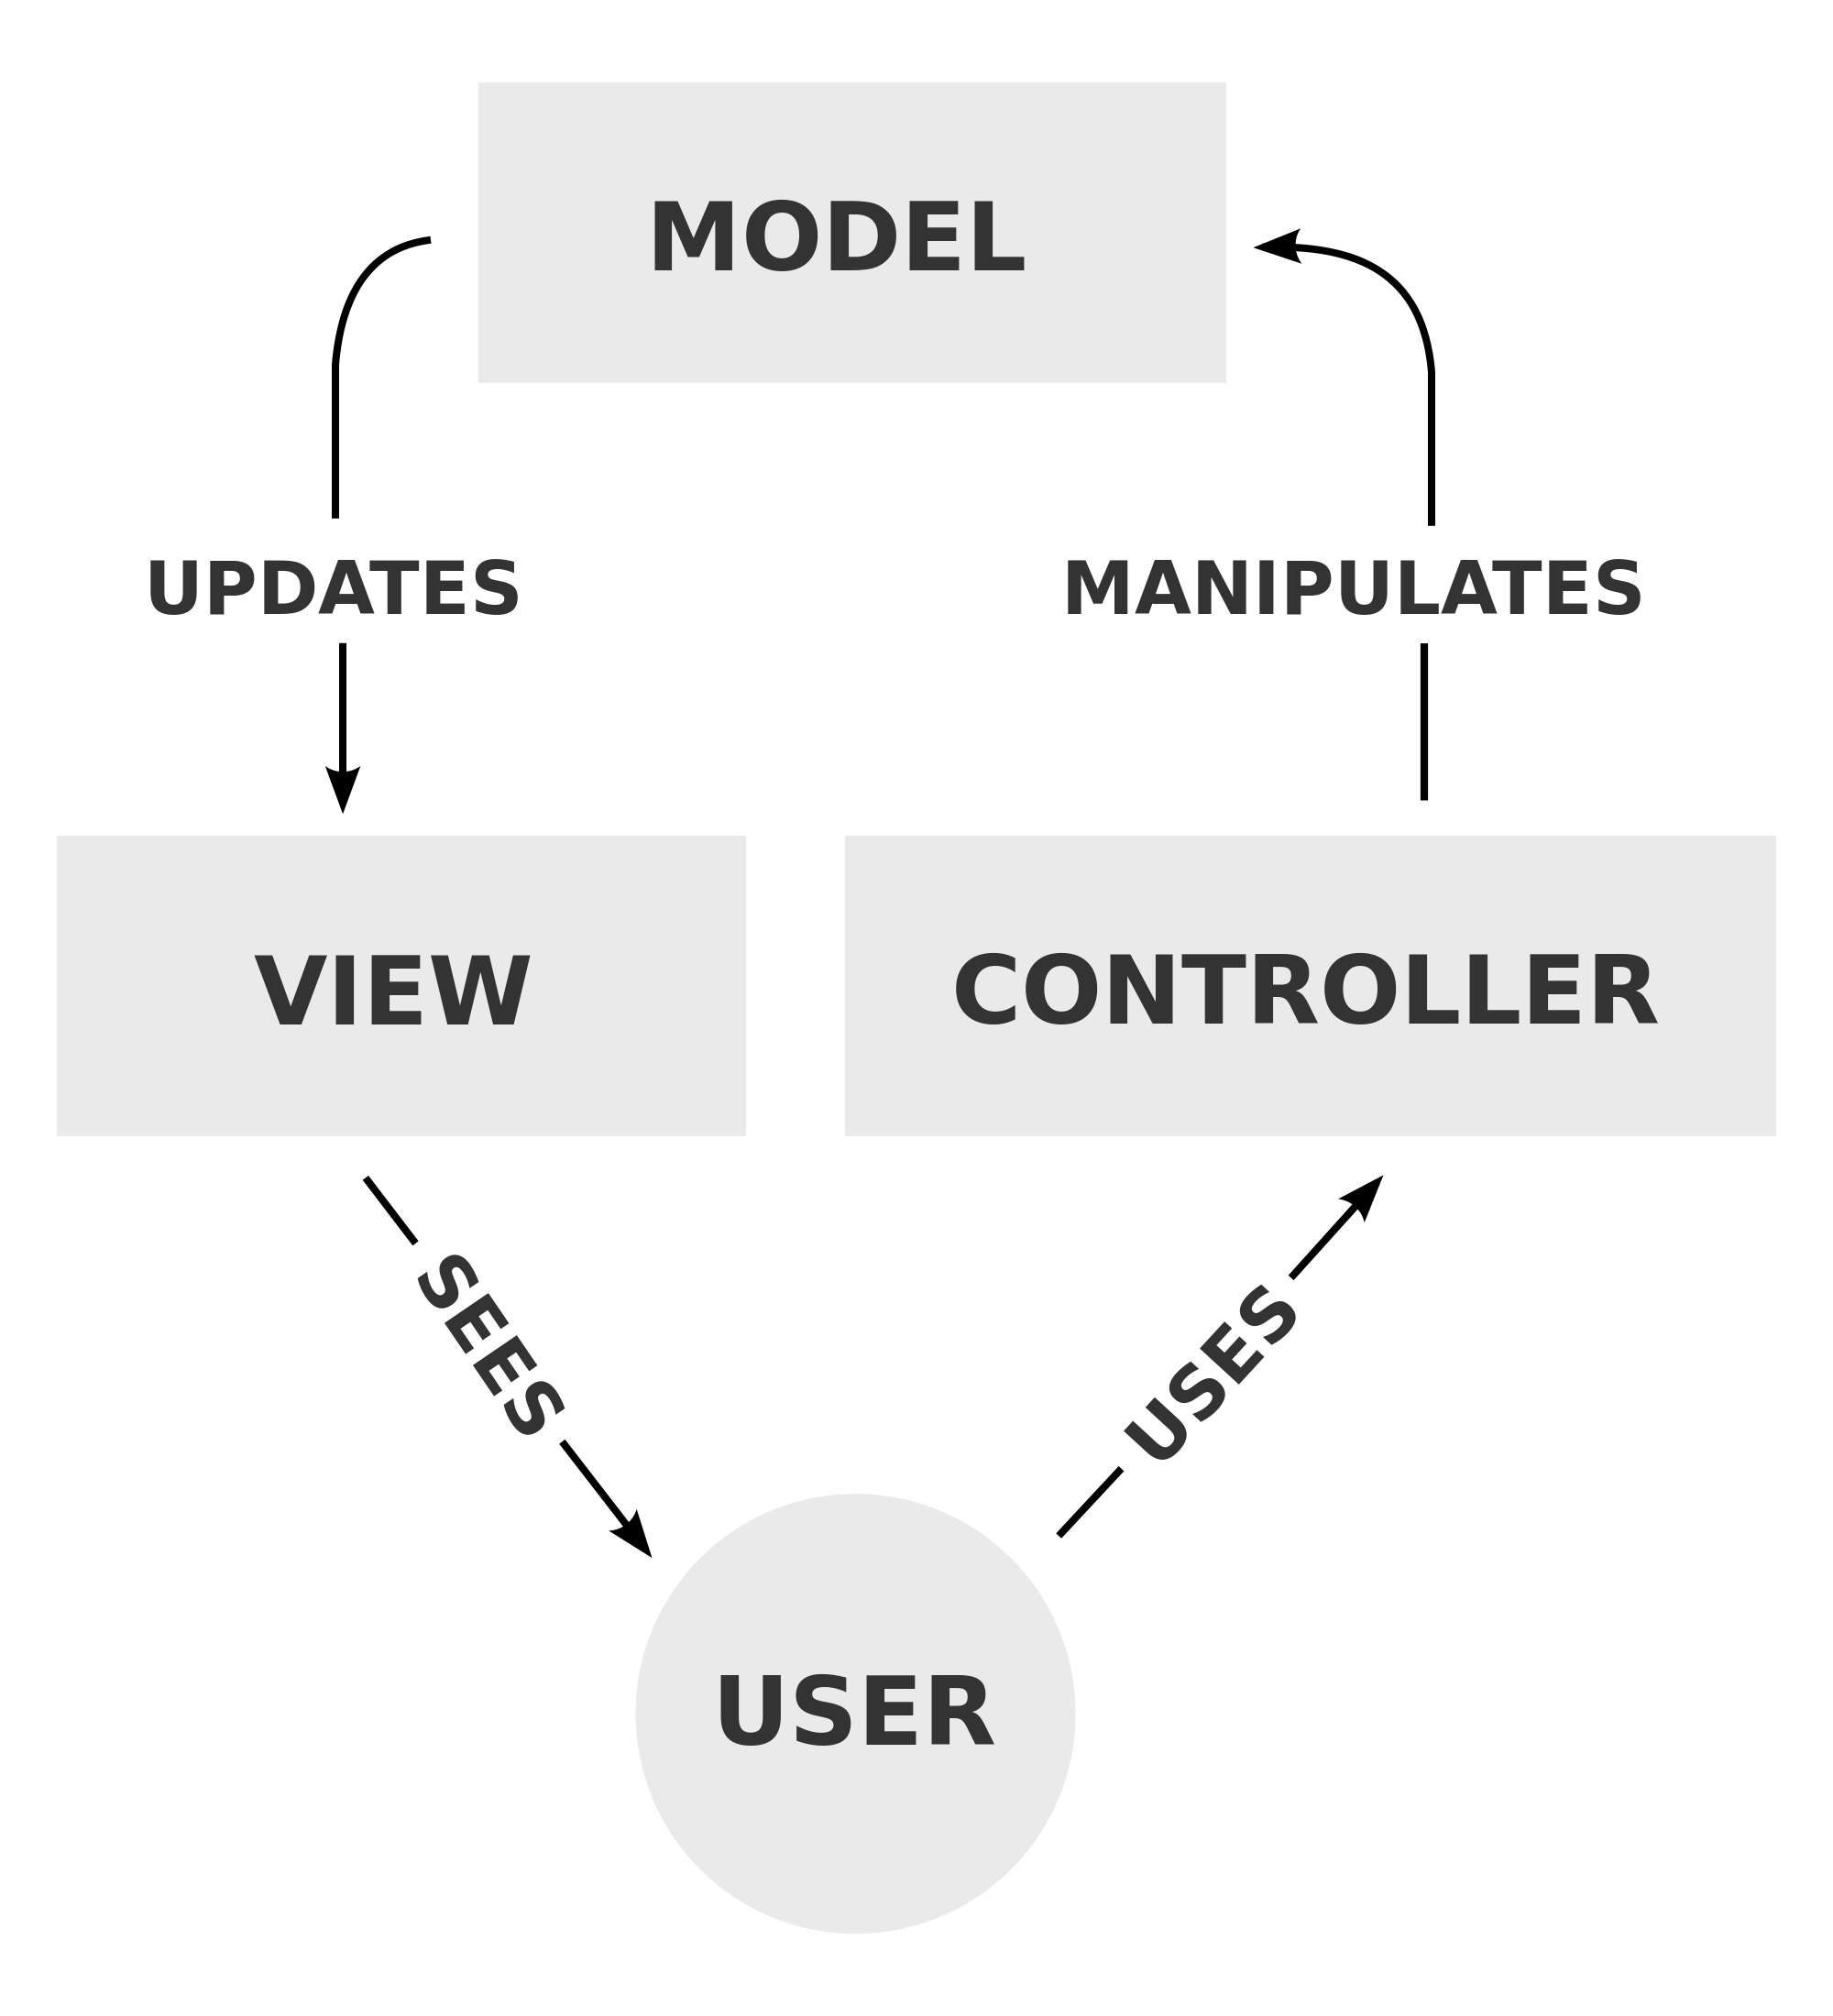
\includegraphics[width =0.4\linewidth, center]{mvc.png}
\caption{Estructura de típica MVC.}
\label{ fig : surface }
\end{figure}
Buscando permitirle a los usuarios compartir y persistir las ecuaciones generadas, se decidió implementar un backend con una base de datos, donde los usuarios puedan almacenar las superficies deseadas junto con un nombre. A su vez la aplicación permite a usuarios ver las ecuaciones que se encuentran almacenadas en la base de datos y mostrar la que se desea. Esta función previamente chequea si hay conectividad con el backend, en caso de no poderse efectuar se deshabilita tanto la opción de grabar como la de cargar.
\\Para la realización de las sombras se decidió utilizar Shadow Map\cite{shadowmap}\cite{realtimerendering}. Este técnica es normalmente utilizada para la realización de sombras dinámicas en los videojuegos\cite{engine}\cite{realtimerendering}. La misma consiste en generar un mapa de profundidad (depth-map) desde la posición de la luz, y utilizarlo a la hora de sombrear cada píxel, comparando la distancia de ese punto contra la obtenida en el mapa de profundidad se decide si esta iluminado por esa luz o no. Este tipo de sombras pueden sufrir problemas de aliasing y de autosombreado (self-shadowing)\cite{realtimerendering}, pero su utilización no produce un gran impacto en la performance.
\\Para la compatibilidad del joystick se decidió utilizar polling de los valores del joystick, esta es la forma comúnmente utilizada en el desarrollo de videojuegos\cite{engine}. Esto consiste en analizar en cada frame los valores de los registros del driver para verificar en que estado se encuentra y actuar de la forma correspondiente.
\\Se decidió agregar un módulo que se encargase de parsear las ecuaciones ingresadas por el usuario, de forma que este las ingresase de la forma más clara posible. Esto se realizó con la intención de tener una interfaz transparente, que permita ingresar las ecuaciones de forma similar a SURFER, y que permita usar algunas funciones como $min, max, abs, etc$.
\\Se optó por permitir a los usuarios generar una cantidad sin límite de ecuaciones, contando con una opción que le permita elegir si quiere visualizar una única o varias. En caso de querer visualizar varias puede hacerlo con la interfaz o utilizando el teclado, donde se mapean las primeras diez ecuaciones a los números de este. 
\\Con la idea de permitir a los usuarios seleccionar la región que se desea recalcular se decidió implementar un método que presenta un cubo, el cual indica la región que se quiere generar.
\begin{figure}[h!]
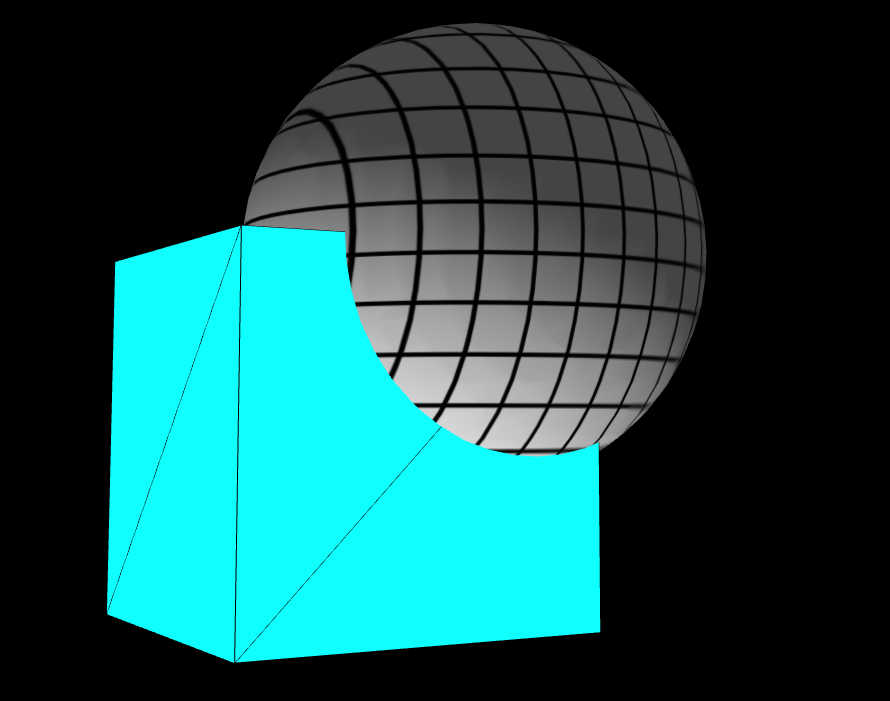
\includegraphics[width =0.45\linewidth]{cubo1.png}
\hfill
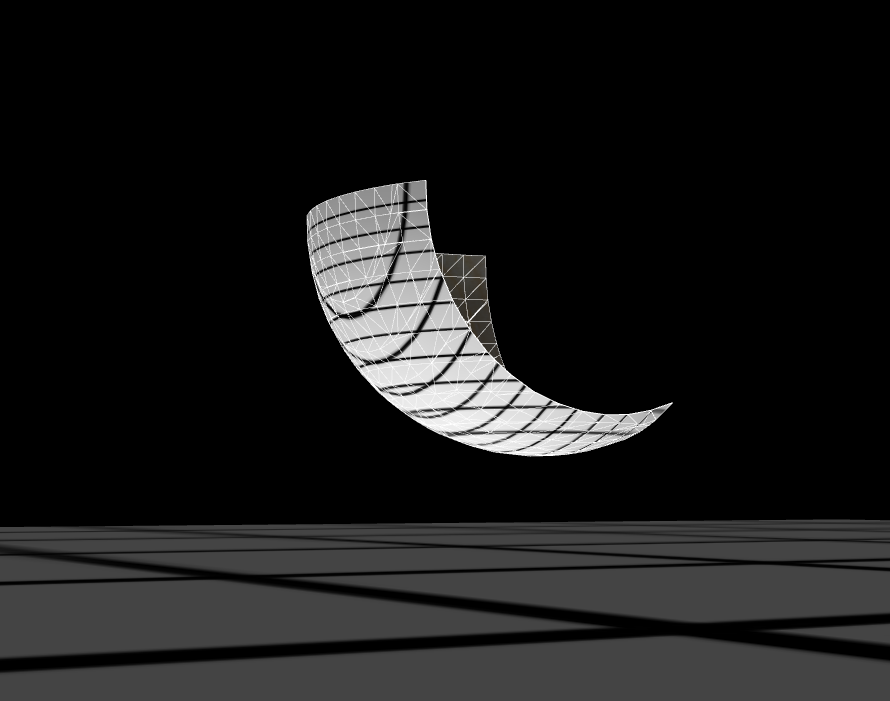
\includegraphics[width =0.45\linewidth]{cubo2.png}
\caption{ A la izquierda se puede apreciar el cubo de zoom y a la derecha el resultado de aplicarlo.}
\label{ fig : surface }
\end{figure}
\section{Solución propuesta}
Como se mencionó anteriormente considerando los resultados obtenidos con las pruebas sobre SURFER  y el hecho de que este utiliza proyección ortográfica, por lo que debería de ser modificado a perspectiva real en caso de querer utilizar tecnologías de realidad virtual, se optó por utilizar de base otro software, particularmente por abandonar los raytracers y utilizar meshers basándose en el trabajo de Mykola Lysenko.
\\La aplicación desarrollada es un visualizador de ecuaciones implícitas web. Esta utiliza THREEJS junto con WebGL, esta fue una decisión importante, ya que permite que la aplicación se pueda ejecutar en todos los navegadores modernos. Esto permite que la aplicación se pueda utilizar por una gran cantidad de jóvenes.
\\Para que la aplicación funcione con Oculus Rift, se utilizó MozVr lo que permite poder utilizar el dispositivo en el navegador Nightly. La aplicación también funciona con Google Cardboard en dispositivos móviles. Esto es una restricción ya que si se desea utilizar la aplicación por sus capacidades estereocópicas en PC se deberá descargar ese navegador con el plugin de MozVR, pero para ver la aplicación en su forma más simple no será necesario.
\\ Para tener una arquitectura MVC bien definida se utilizó AngularJS. Se decidió utilizar este framework con la intención de que la arquitectura obtenida fuese más clara y extendible de manera más sencilla.  XXX PONER BASTANTE DE ESO
\\El sitio desarrollado utiliza los algoritmos presentados anteriormente basados en el trabajo de Mykola Lysenko\cite{mykola1}\cite{mykola2} para generar una malla poligonal de las ecuaciones ingresadas por el usuario con el paso seleccionado por este. El paso se usa para la definición de la grilla sobre la cual se generará la malla, esta genera dividiendo el intervalo ingresado de manera que cada sección de la grilla posea la medida del paso. Se trabajó sobre el código de Lysenko y se le realizaron una serie de modificaciones para que funcionase con THREEJS, particularmente en la versión 73. Además de esas modificaciones, a la geometría devuelta por estos algoritmos, se les calculó las normales en de sus vértices, esto cómo se explicó previamente permite que la visualización no sea facetada, lo que permite que la ecuación sea visualmente más atractiva. 
\\La geometría obtenida es mostrada en una escena tridimensional, que puede ser navegada por el usuario de distintos modos, así como se le puede modificar varios parámetros, como la luz, la textura de la ecuación y hasta puede aplicarle efectos generados por shaders programados en GLSL.
\\Se decidió utilizar GLSL por su gran flexibilidad, ya que es el lenguage para la realización de shaders de openGL, además de por su interacción con THREEJS. Con este lenguaje se implementaron varios efectos interesantes, entre ellos se encuentran lava, agua y gelatina.  Se implementaron vertex shaders, mini programas responsables de devolver la posición de cada vértice de la geometría, para realizar efectos como la vibración en la gelatina. A su vez se utilizaron fragment shaders, mini programas encargados de retornar un color para un segmento de la superficie, para generar efectos como el de la textura del agua que actúa como si estuviese animada para generar la sensación de olas.
\\Para la utilización de texturas, se les debió asignar coordenadas de mapeo UV a las geomtrías. Esto se debe a que la forma de proyectar texturas consiste en asignarle coordenadas a cada vértice de en que sector de la textura pertenece. Estas coordenadas son interpoladas utilizando la interpolación en perspectiva para las caras\cite{realtimerendering}\cite{engine}. Para asignarles coordenadas se utilizó la proyección planar\cite{realtimerendering}.
\begin{figure}[h!]
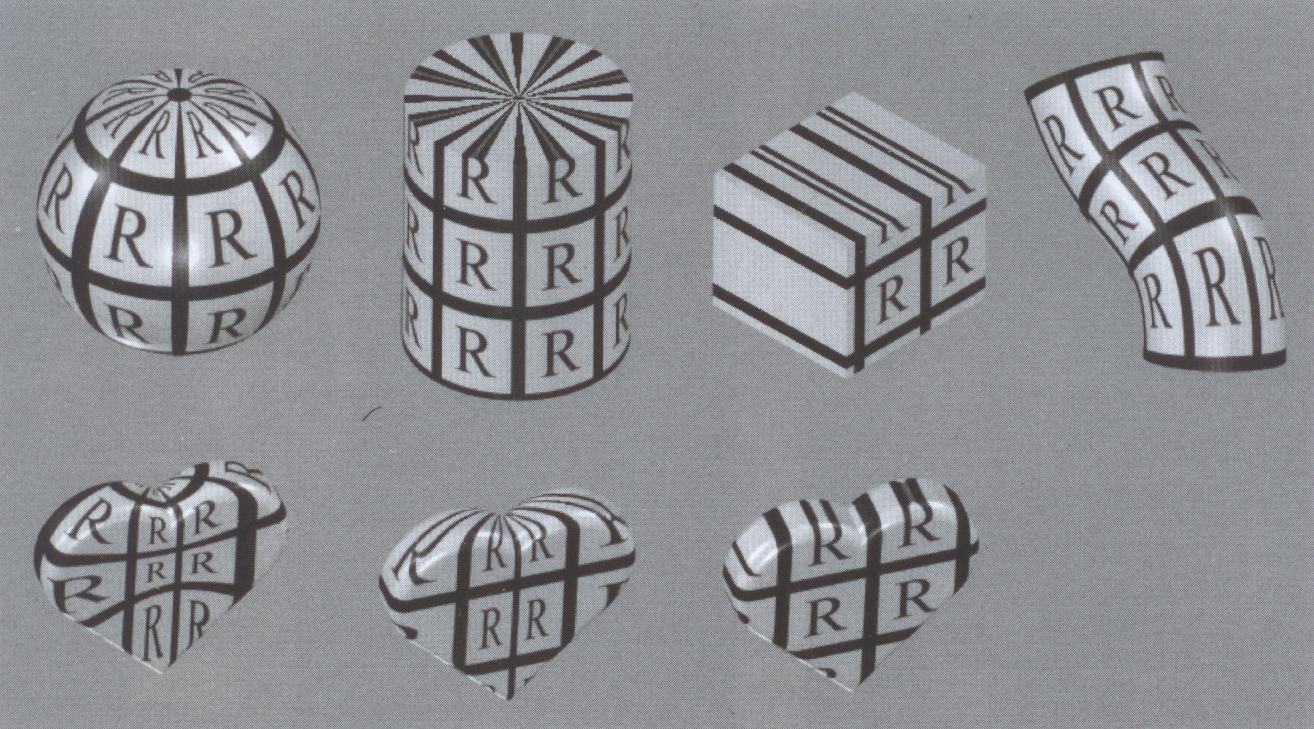
\includegraphics[width =0.7\linewidth, center]{proyecciones.png}
\caption{Tipos de proyección. De izquierda a derecha, esférica, cilíndrica, planar y natural.}
\label{ fig : surface }
\end{figure}
\\Se optó por este tipo de proyección ya que a diferencia de la natural, la cual debe realizarse de forma manual, es posible de automatizar, de forma de que se generen las coordenadas de manera dinámica. Se prefirió ante las esféricas y las cilíndricas, dado de que estas sólo se ven de forma agradable sobre las figuras para las que están pensadas. En general notamos que la proyección planar conseguía mejores resultados. 
\\Hay que recordar que los algoritmos generan una aproximación de la superficie, por lo que no es el método más exacto de visualizarlas, pero al no usar raytracing y usar WebGL, la experiencia visual se ve mejorada. Es decir tanto el framerate como la resolución son más que aceptables para la visualización estereoscópica. Estas dos cosas son muy importantes para el uso de dispositivos de realidad virtual, ya que tasas de refresco bajas pueden provocar mareos, incomodidad y hasta vómitos como se mencionó anteriormente.
\\La página permite la visualización de varias ecuaciones a la vez, con diferentes texturas y materiales. También permite seleccionar de forma visual la zona de la ecuación que se quiere poligonizar.
\\Otra funcionalidad que posee es el almacenamiento en una base de datos de las ecuaciones que los usuarios consideren interesantes, almacenando un nombre además de la ecuación y su geometría. Esto es interesante ya que permite que se compartan ecuaciones interesantes y se trabaje en conjunto en la búsqueda de determinadas ecuaciones. Para hacer esta funcionalidad se implementó un backend el cual maneja la base de datos e interactúa con el cliente web.
\\Como se mencionó anteriormente se puede utilizar Google Cardboard o Oculus Rift para experimentar la escena en realidad virtual, pudiendo ver las ecuaciones, aprovechando las técnicas de estereoscopía, con una mayor inmersión.
\\Utilizando la Gamepad API\cite{gamepadapi} la aplicación es compatible con un joystick de XBOX ONE, el cual es usado para navegar la escena cuando se está utilizando el Oculus Rift. El uso del joystick de XBOX ONE (joystick oficial de Oculus Rift, el cual viene incluido actualmente en la versión de consumidor), junto con el Oculus permite atraer la atención de jóvenes hacia la aplicación y por consiguiente hacia la matemática. La API permite acceder de forma intuitiva a los registros del driver\cite{engine}, lo que permite realizar polling para verificar en cada frame en que estado se encuentra el mismo.
\\Sí se accede desde una computadora a la aplicación, las ecuaciones proyectan sombras, no sólo contra el “piso” sino que sobre sí mismas. Por motivos de optimización se decidió sacar esta funcionalidad cuando se ingresa desde celulares, ya que esta operación disminuye significativamente el framerate que se obtiene en los dispositivos móviles, esto se debe a que estos dispositivos no están pensados para este tipo de aplicación. Como se mencionó anteriormente las sombras se generan utilizando la técnica de Shadow Map\cite{shadowmap}\cite{realtimerendering}.
\\El usuario puede cambiar parámetros de qué luces están activas, así como mover una de las luces de forma de poder observar mejor la ecuación. Esto permite ver en tiempo real la variación de la sombra, así como los efectos de la luz sobre la ecuación. 
\\La ecuación se visualiza normalmente en un modo donde la cámara “orbita” alrededor de ella, pero cuando se ingresa al modo de realidad virtual, se visualiza como si fuese en primera persona. Cuando se encuentra en dicho modo se puede usar tanto el teclado como el joystick para desplazarse alrededor de la escena de forma de poder recorrerla completamente. Esto le da gran libertad al usuario y permite que explore librementa la escena pudiendo observar una gran cantidad de detalles que no son posibles de otra forma.
\\Para la versión móvil la figura se encuentra desplazándose circularmente, esto permite que se pueda visualizar de todos los ángulos en el modo de realidad virtual sin tener que dejar de utilizar el Google Cardboard para poder utilizar la pantalla táctil.
\clearpage
\subsection{Arquitectura}
Como se mencionó anteriormente la aplicación cuenta con un cliente web, un backend y una base de datos. En esta sección se presentan las arquitecturas del cliente web y del backend, así como la estructura de la base de datos.
\subsubsection{Cliente web}
A continuación se presenta una versión simplificada del cliente web, y se provee una breve descripción de algunos de los módulos más importantes del mismo.\\
\begin{figure}[h]
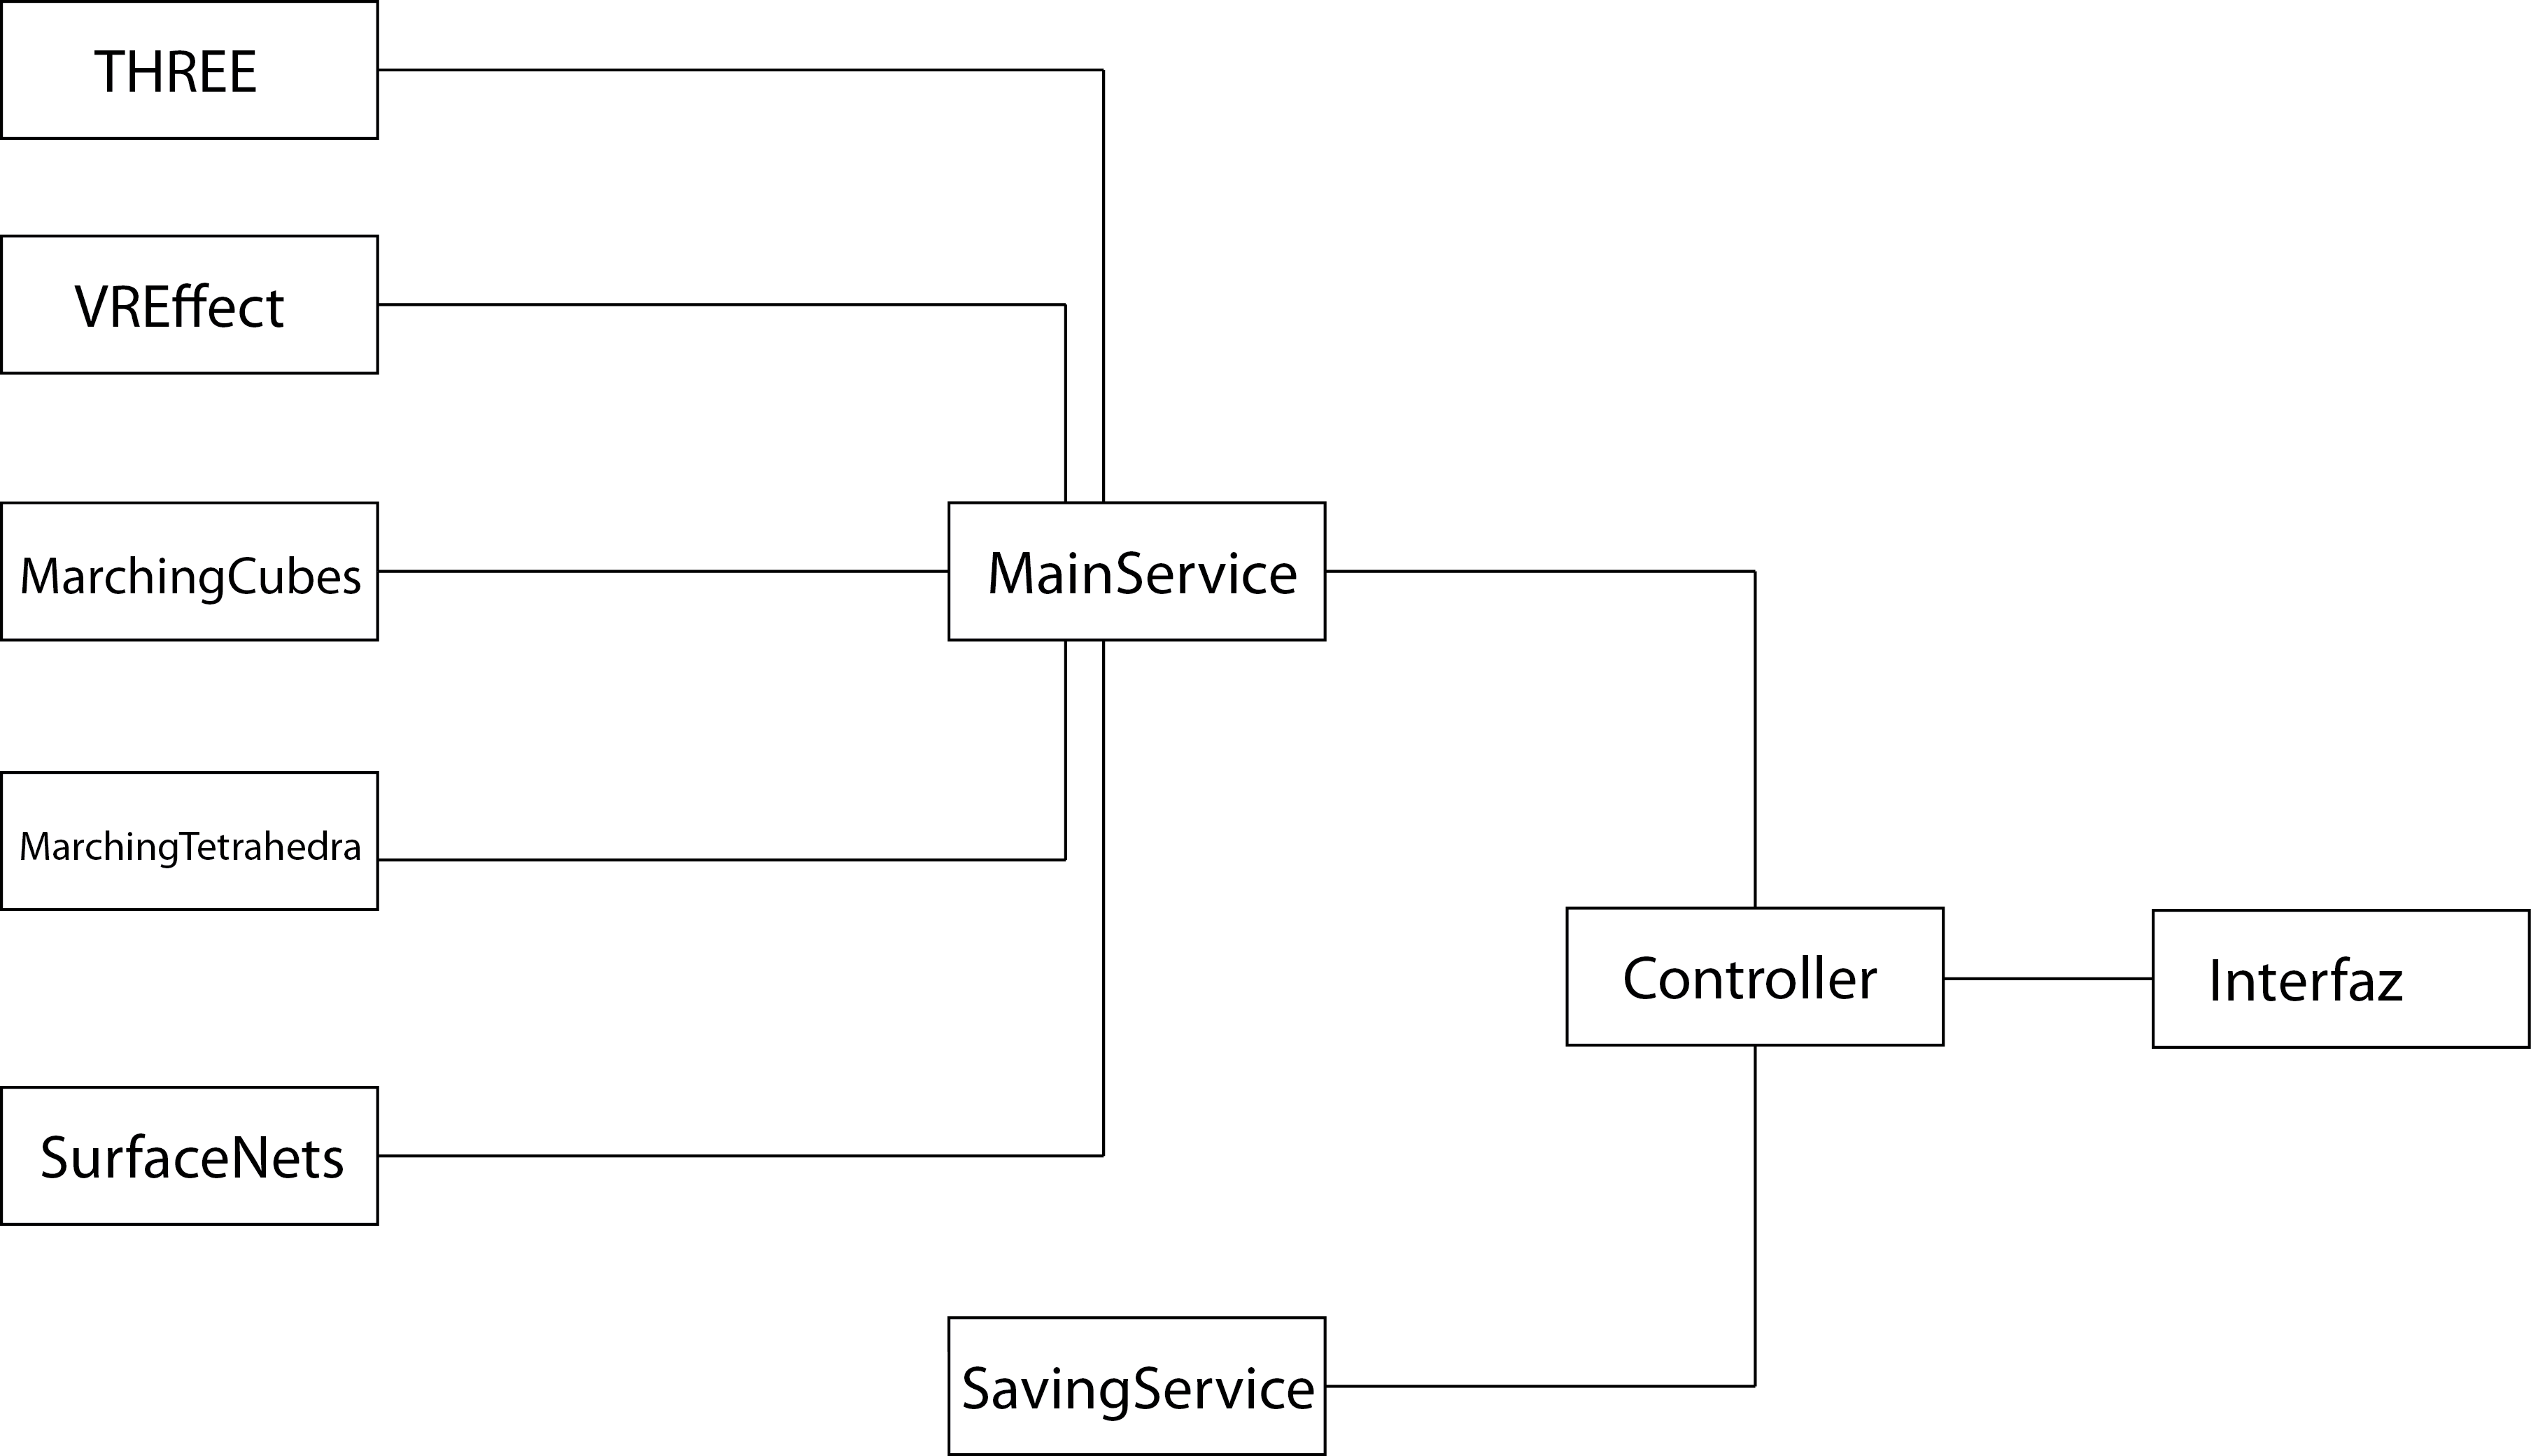
\includegraphics[width=\textwidth]{arq_sim.png}
\caption{Arquitectura del cliente web.}
\end{figure}
\\La aplicación cuenta con dos services y un controller para una única vista. 
\\El SavingService es el responsable de comunicarse con el backend para tanto almacenar como cargar las mallas junto con su información asociada. Este módulo es utilizado por el Controller, el cual utilizando las interfaces del MainService le proporciona a éste la información de la malla que se recuperó de la base de datos.
\\El MainService es el responsable de generar las mallas, crear la escena, hacer las actualizaciones y efectuar el render. Este módulo es el se comunica con más módulos, ya que es el que realiza las tareas más importantes y difíciles. También es el responsable de mostrar las ecuaciones que sean pertinentes, es decir sólo aquellas que deban ser visibles en el momento dado. En este módulo se generan las coordenadas de mapeo UV, se generan los shaders, se ejecuta el main loop de la aplicación, se generan las superficies, se realizan todas las actualizaciones (posición de cámara, posición de luz, etc), se generan las texturas, genera el cubo de zoom para recalcular la zona de la superficie que se quiera. Este es el módulo principal de la aplicación, que utilizando el resto, efectúa la mayoría de las operaciones importantes.
\\El Controller es el responsable de manejar la interfaz y usar los servicios que le son provistos.
\\MarchingCubes implementa el algoritmo para generar la malla del mismo nombre, es invocado por el MainService.
\\MarchingTetrahedra es similar a MarchingCubes, en cuanto implementa a un algoritmo para generar la malla y que es invocado por el servicio principal.
\\SurfaceNets es análogo a los dos módulos mencionados previamente, implementa el algoritmo de Naive SurfaceNets.
\\AngularJS es un framework diseñado para generar paginas web dinámicas, y el mismo extendie la sintaxis utilizada por HTML y separa la logica de acceso a los elementos HTML, de la logica misma de la aplicación, haciendo la aplicación mas sencilla de testear y entender. En este proyecto se utilizó para facilitar las comunicaciones entre la interfaz del menu con el servidor de backend y el MainService.
\\Bootstrap es un framework enfocado en el diseño de sitios web, brindando diversos componentes comumnmente utilizado en otros sitios. Además contiene diversos templates, plantillas y objetos con diseños modernos y atractivos. 
\\THREEJS es la librería presentada anteriormente, que actúa como wrapper de WebGL e implementa algunas funcionalidades de modo de permitir un uso más simple. A su vez cuenta con la ventaja de que garantiza el funcionamiento de la aplicación en los navegadores actuales, esto permite que la misma esté disponible para la mayor cantidad de gente posible.
\\VREffect es el módulo que se encarga de realizar el efecto estereoscópico, cuando la aplicación se encuentra en modo VR, se le invoca para que utilizando los parámetros que obtiene del navegador genere las dos imágenes con la distorsión necesaria para el dispositivo que se está utilizando.
\\VRControls es el responsable de que cuando se está en modo VR, tome del dispositivo la rotación de forma de mover la cámara de la misma forma, para poder dar la sensación de inmersión.
\\Gamepad tiene el objetivo de exponer el estado del joystick de XBOX ONE utilizando la Gamepad API\cite{gamepadapi} a el MainService.
\\Parser se encarga de parsear las ecuaciones ingresadas por el usuario, de manera de proveerle al MainService las ecuaciones de la forma que los algoritmos necesitan como entrada. Este módulo permite que el usuario no se preocupe de como requieren los algoritmos de que se escriba la ecuación.
\subsubsection{Backend y base de datos}
El backend de la aplicación fue realizado en el lenguaje Python con el framework de django y django rest framework para comunicarse con los clientes web. Este se encarga de guardar datos de las superficies que se consideren interesantes, por ejemplo: coordenadas, nombre, cantidad de caras, etc. Todo esto se encuentra guardado en la base de datos Postgres.
\\Esta parte de la aplicación presenta una ventaja sobre otro tipo de aplicaciones similares, ya que permite que usuarios de distinta parte del compartan ecuaciones interesantes. Además de que a medida de que más usuarios generar y almacenan ecuaciones la aplicación va creciendo en cuanto al catálogo de ecuaciones que ofrece.
\clearpage
\subsection{Interfaz}
En este punto se muestran los distintos modos con los que se puede interactuar con la aplicación. Esta punto es una breve descripción, se puede encontrar más información en el Anexo C.
\subsubsection{Menú lateral}
La aplicación cuenta con un menú lateral, donde se puede controlar una serie de parámetros. En ese menú se ingresa la ecuación, así como se configuran una serie de parametros, como la zona que se quiere generar, el paso del algoritmo, que algoritmo se desea utilizar,etc. 
\subsubsection{Mensajes}
La interfaz también cuenta con una serie mensajes. Estos son pequeños carteles que aparecen arriba la derecha, al momento de ingresar a la página se muestra un mensaje de bienvenida en verde. 
\\El manejo de errores de la aplicación se hace utilizando el mismo sistema de mensajes. En el momento en el que acontece un error se muestra en la misma posición que el mensaje de bienvenida un cartel explicando el error pero con fondo rojo. Los errores pueden variar en cuanto al tipo, por ejemplo el error podría ser que el usuario ingreso una ecuación cuyos paréntesis están desbalanceados.
\subsubsection{Teclado y Mouse}
También se puede interactuar con la aplicación utilizando el teclado y el mouse, aunque el uso del teclado para afectar la escena puede ser habilitado/deshabilitado utilizando el menú lateral mencionado previamente.
\\El mouse se utiliza principalmente para controlar la cámara cuando no se esta utilizando Oculus Rift. La aplicación cuenta con dos modos, uno en el cual se orbita alrededor de la ecuación y otro donde la cámara se comporta como si fuese en primera persona, es decir permitiendo mirar hacia los costados fijando la posición de la misma.
\\Por otra parte se puede utilizar el teclado para una gran cantidad de funciones. Entre ellas se encuentra desplazarse, mover las luces, cambiar el material de la ecuación, cambiar la ecuación, activar/desplazar/agrandar/achicar el cubo de zoom, etc. La matoría de las funciones de la aplicación se pueden realizar apretando una serie de teclas desde el teclado.
\\Para más información la función de cada una de las teclas dirigirse al Anexo C, donde se encuentra un manual de usuario.
\clearpage
\subsubsection{Joystick}
La aplicación también se puede utilizar con el joystick de XBOX ONE. El cual permite, cuando se encuentra en modo VR, desplazarse de forma más intuitiva y cómoda que si se utilizase el teclado. El mismo puede conectarse de forma inalámbrica.\\
\begin{figure}[h!]
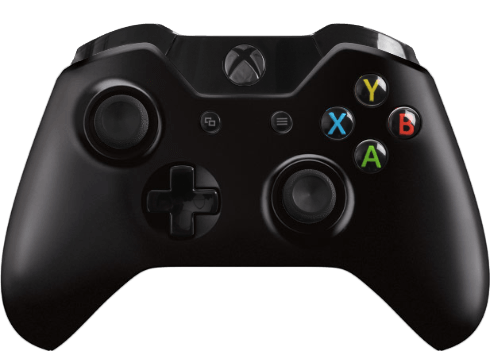
\includegraphics[width=0.7\textwidth,center]{joystickPosta.png}
\caption{Joystick de XBOX ONE.}
\end{figure}
\\El joystick permite una gran flexibilidad ya que puede utilizarse de forma más sencilla que un teclado cuando se esta utilizando el Oculus Rift. Esto se debe en parte, en que es más simple para la mayoría de los usuarios detectar donde se encuentran los botones sin mirar por su forma ergonómica que en un teclado. Por este motivo esto aumenta significativamente el grado de usabilidad de la aplicación, ya que se vuelve más sencilla de utilizar para los usuarios, principalmente para los jóvenes que tienen mayor experiencia con un joystick.
\clearpage
\section{Pruebas}
En esta sección se presentan las pruebas que realizamos sobre el sistema, así como los resultados obtenidos. Las pruebas se dividen en cinco tipos, el primero es una comparación entre la performance y los resultados obtenidos utilizando cada uno de los 3 algoritmos. El segundo tipo, es cuantos fps se lograron obtener para una serie de ecuaciones, considerando la cantidad de polígonos que había en la escena. El tercero es una comparación entre SURFER y nuestra aplicación cuando se trata de puntos singulares, estos son los puntos donde nuestra aplicación genera algunos artefactos. Los últimos dos tipos son una serie de operaciones interesantes que permite realizar la aplicación y una galería de imágenes.
\subsection{Hardware utilizado}
Las pruebas en PC se realizaron sobre un Notebook Alienware M17xR4. El cual cuenta con un procesador Intel I7-3840QM de 2.8 GHz con Turboboost hasta 3.8 GHz. La memoria RAM es de 32 GB de 1777 MHz, y cuenta con una tarjeta de video nVidia 680M.
\\Se utilizó un DK1 y un DK2 como dispositivos de realidad virtual.
\\En las plataformas móviles, se utilizó un Samsung  Galaxy S5 y un Samsung  Galaxy Note3, junto con un Google Cardboard. 

\subsection{Software utilizado}
En PC la aplicación se testeo utilizando Firefox Nightly 48.0a1 con el plugin Mozilla WebVR plus 0.5.0. Se utilizó el runtime de Oculus 0.8.0.0. Todo se corrió sobre Windows 10.
\\En los teléfonos celulares se ejecutó sobre Google Chrome.

\subsection{Comparación entre meshers}
\subsubsection{Comparación a través de sucesiones}
La primer prueba que realizamos fue fijando la bounding box y el paso del algoritmo, utilizar una sucesión de superficies y utilizar los tres algoritmos y registrar sus tiempos. Este tipo de comparación fija la información de la función que se utiliza para la generación de la malla, pero los distintos algoritmos generan distinta cantidad de caras.
\\Se utilizó como límites $[-4,4]$ en los tres ejes, y el paso fue 0.05. La sucesión que se utilizó fue $cos(\frac{n\pi x}{2}) + cos(\frac{n\pi y}{2}) +cos(\frac{n\pi z}{2}) =0$. Los tiempos de la tabla son en segundos y son los promedios de 10 ejecuciones.
\begin{table}[h!]
  \centering
  \label{tab:table1}
  \begin{tabular}{cccc}
    \toprule
    Valor de n & Surface Nets & Marching Tetrahedra & Marching Cubes\\
    \midrule
    1 & 2.859 & 19.276 & 3.937\\
    2 & 5.406 & 42.7 & 15.972\\
    3 & 11.348 & 105.802 & 25.328\\
    \bottomrule
  \end{tabular}
  \caption{Primera comparación con sucesiones.}
\end{table}
\\Luego se decidió utilizar la misma sucesión pero achicando los límites de manera que los tiempos fueran menores, con el fin de poder realizar una mayor cantidad de ejecuciones por nivel y obtener una mayor significancia estadística, esta vez se ejecutaron 15 veces. Los límites se cambiaron a $[-1,1]$. \\
\begin{table}[h!]
  \centering
  \label{tab:table1}
  \begin{tabular}{cccc}
    \toprule
    Valor de n & Surface Nets & Marching Tetrahedra & Marching Cubes\\
    \midrule
    1 & 0.016 & 0.029 & 0.022\\
    2 & 0.08 & 0.375 & 0.091\\
    3 & 0.088 & 0.534 & 0.132\\
    4 & 0.196 & 0.618 & 0.311\\
    5 & 0.134 & 0.822 & 0.345\\
    6 & 0.178 & 1.203 & 0.349\\
    7 & 0.189 & 1.384 & 0.432\\
    8 & 0.22 & 1.434 & 0.478\\
    9 & 0.238 & 1.565 & 0.52\\
    10 & 0.345 & 1.84 & 0.671\\
    \bottomrule
  \end{tabular}
  \caption{Segunda comparación con sucesiones.}
\end{table}
\\Luego para comparar el tiempo que lleva generar la superficies con cada algoritmo cuando la cantidad de caras es similar, se crearon las mismas ecuaciones pero con distintos pasos. Esto se debe a que en general Marching Tetrahedra genera 3 veces más que los otros dos algoritmos. Se utilizó 0.05 como paso en Marching Cubes y Naive Surface Nets; mientras que 0.085 para Marching Tetrahedra. Como las ejecuciones anteriores para Naive Surface Nets y Marching Cubes ya utilizaban ese pasa sólo se ejecutó denuevo la parte de Marching Tetrahedra.
\begin{table}[h!]
  \centering
  \label{tab:table1}
  \begin{tabular}{cccc}
    \toprule
    Valor de n & Surface Nets & Marching Tetrahedra & Marching Cubes\\
    \midrule
    1 & 0.016 & 0.017 & 0.022\\
    2 & 0.08 & 0.156 & 0.091\\
    3 & 0.088 & 0.191 & 0.132\\
    4 & 0.196 & 0.288 & 0.311\\
    5 & 0.134 & 0.324 & 0.345\\
    6 & 0.178 & 0.389 & 0.349\\
    7 & 0.189 & 0.413 & 0.432\\
    8 & 0.22 & 0.455 & 0.478\\
    9 & 0.238 & 0.596 & 0.52\\
    10 & 0.345 & 0.794 & 0.671\\
    \bottomrule
  \end{tabular}
  \caption{Comparación con sucesiones a similar cantidad de caras.}
\end{table}
\clearpage
\subsubsection{Comparación a través de ecuaciones puntuales}
A continuación realizamos ciertas ecuaciones con los tres algoritmos con la intención de observar cómo se comportan, y cuál produce mejores resultados visuales. El orden de las imágenes es análogo a la tabla. Para mostrar esto además de las imágenes comparativas se colocan tablas que contienen la cantidad de vértices y caras que contiene cada figura para cada algoritmo. Las caras son todas triangulares, por lo que surface nets que genera caras rectangulares se están contando cada una como dos (se parten en dos triángulos).
\\Primero se realizó una esfera con el paso en 0.1.
\begin{table}[h!]
  \centering
  \label{tab:table1}
  \begin{tabular}{cccc}
    \toprule
    & Surface Nets & Marching Tetrahedra & Marching Cubes\\
    \midrule
    Cantidad de vértices & 392 & 6840 & 1560\\
    Cantidad de caras & 780 & 2280 & 776\\
    \bottomrule
  \end{tabular}
  \caption{Comparación de cantidad de caras y vértices de la esfera utilizando los 3 algoritmos.}
\end{table}
\begin{figure}[h!]
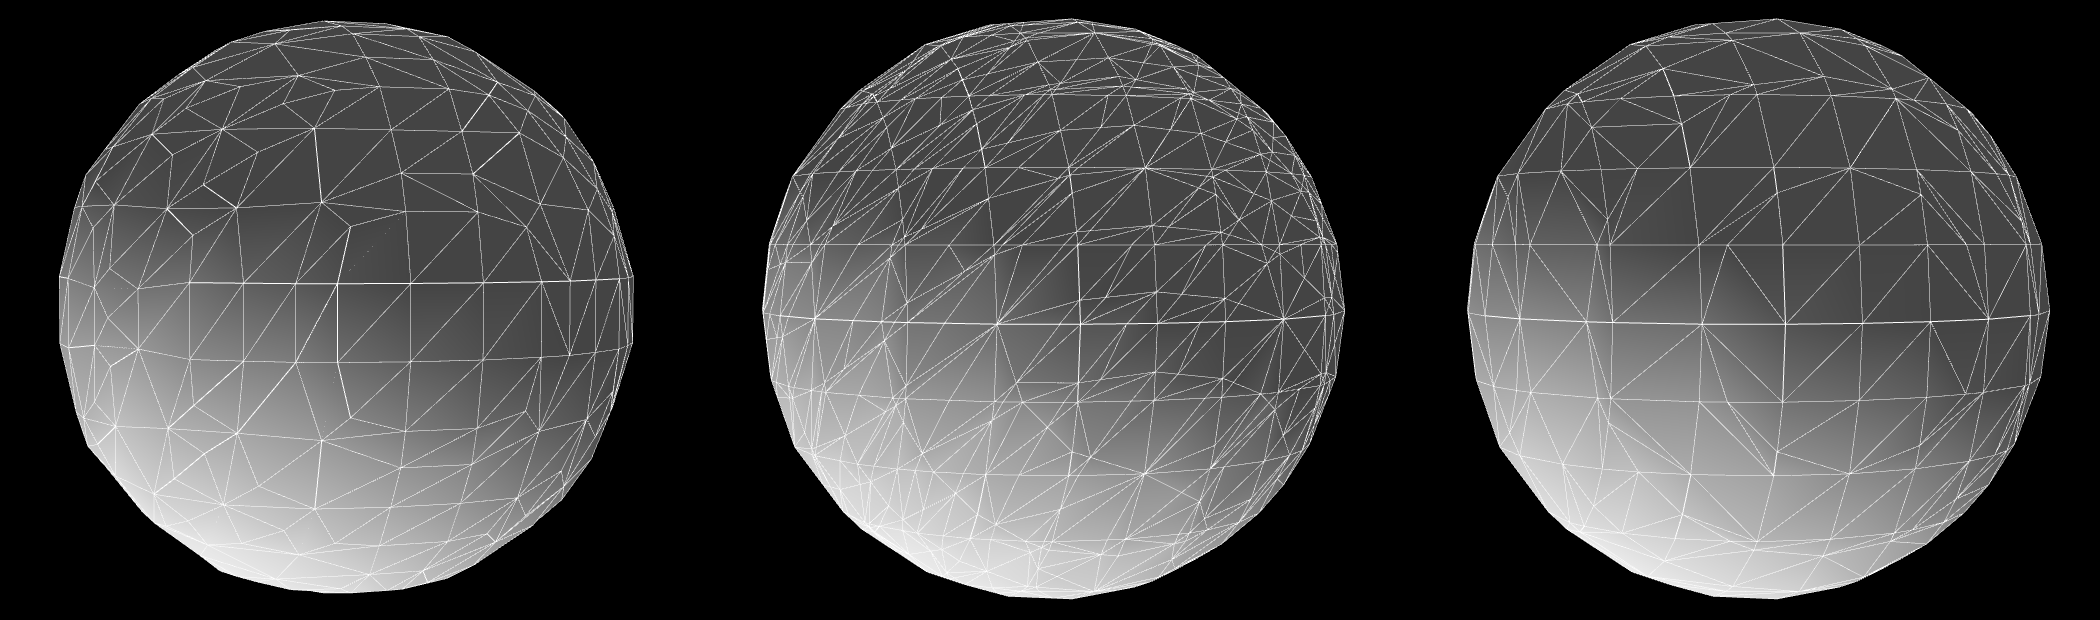
\includegraphics[width=\linewidth,center]{compec1.png}
\caption{Esfera generada utilizando los 3 algoritmos.}
\end{figure}
\\Se puede apreciar en el sector superior a la derecha como Marching Tetrahedra genera una superficie más suave que los otros dos.
\\Con una segunda ecuación se obtuvo lo siguiente con un paso de 0.05.
\begin{table}[h!]
  \centering
  \label{tab:table1}
  \begin{tabular}{cccc}
    \toprule
    & Surface Nets & Marching Tetrahedra & Marching Cubes\\
    \midrule
    Cantidad de vértices & 23432 & 430128 & 94368\\
    Cantidad de caras & 47184 & 143376 & 47504\\
    \bottomrule
  \end{tabular}
  \caption{Comparación de cantidad de caras y vértices utilizando los 3 algoritmos.}
\end{table}
\begin{figure}[h!]
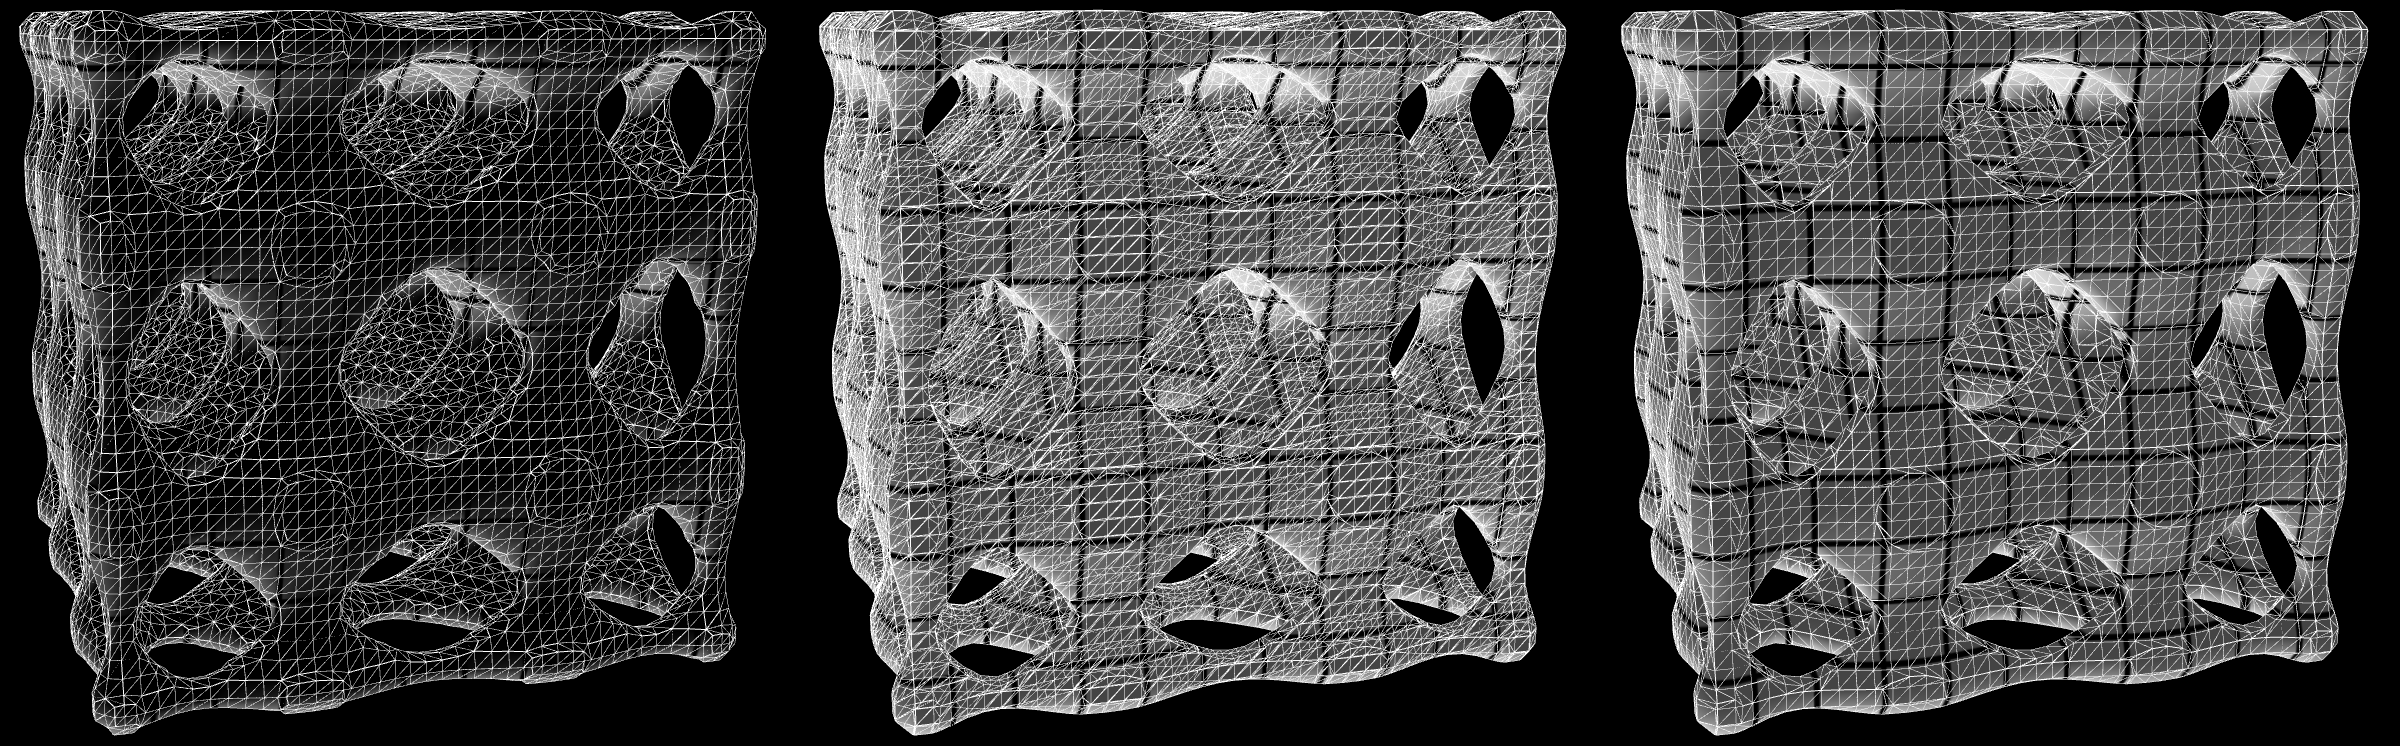
\includegraphics[width=\linewidth,center]{compec2.png}
\caption{Ecuación generada utilizando los 3 algoritmos.}
\end{figure}
\\Finalmente con un cilindro se obtuvo los siguiente y paso 0.1.
\begin{table}[h!]
  \centering
  \label{tab:table1}
  \begin{tabular}{cccc}
    \toprule
    & Surface Nets & Marching Tetrahedra & Marching Cubes\\
    \midrule
    Cantidad de vértices & 3578 & 75960 & 14304\\
    Cantidad de caras & 7152 & 25320 & 7148\\
    \bottomrule
  \end{tabular}
  \caption{Comparación de cantidad de caras y vértices del cilindro utilizando los 3 algoritmos.}
\end{table}
\begin{figure}[h!]
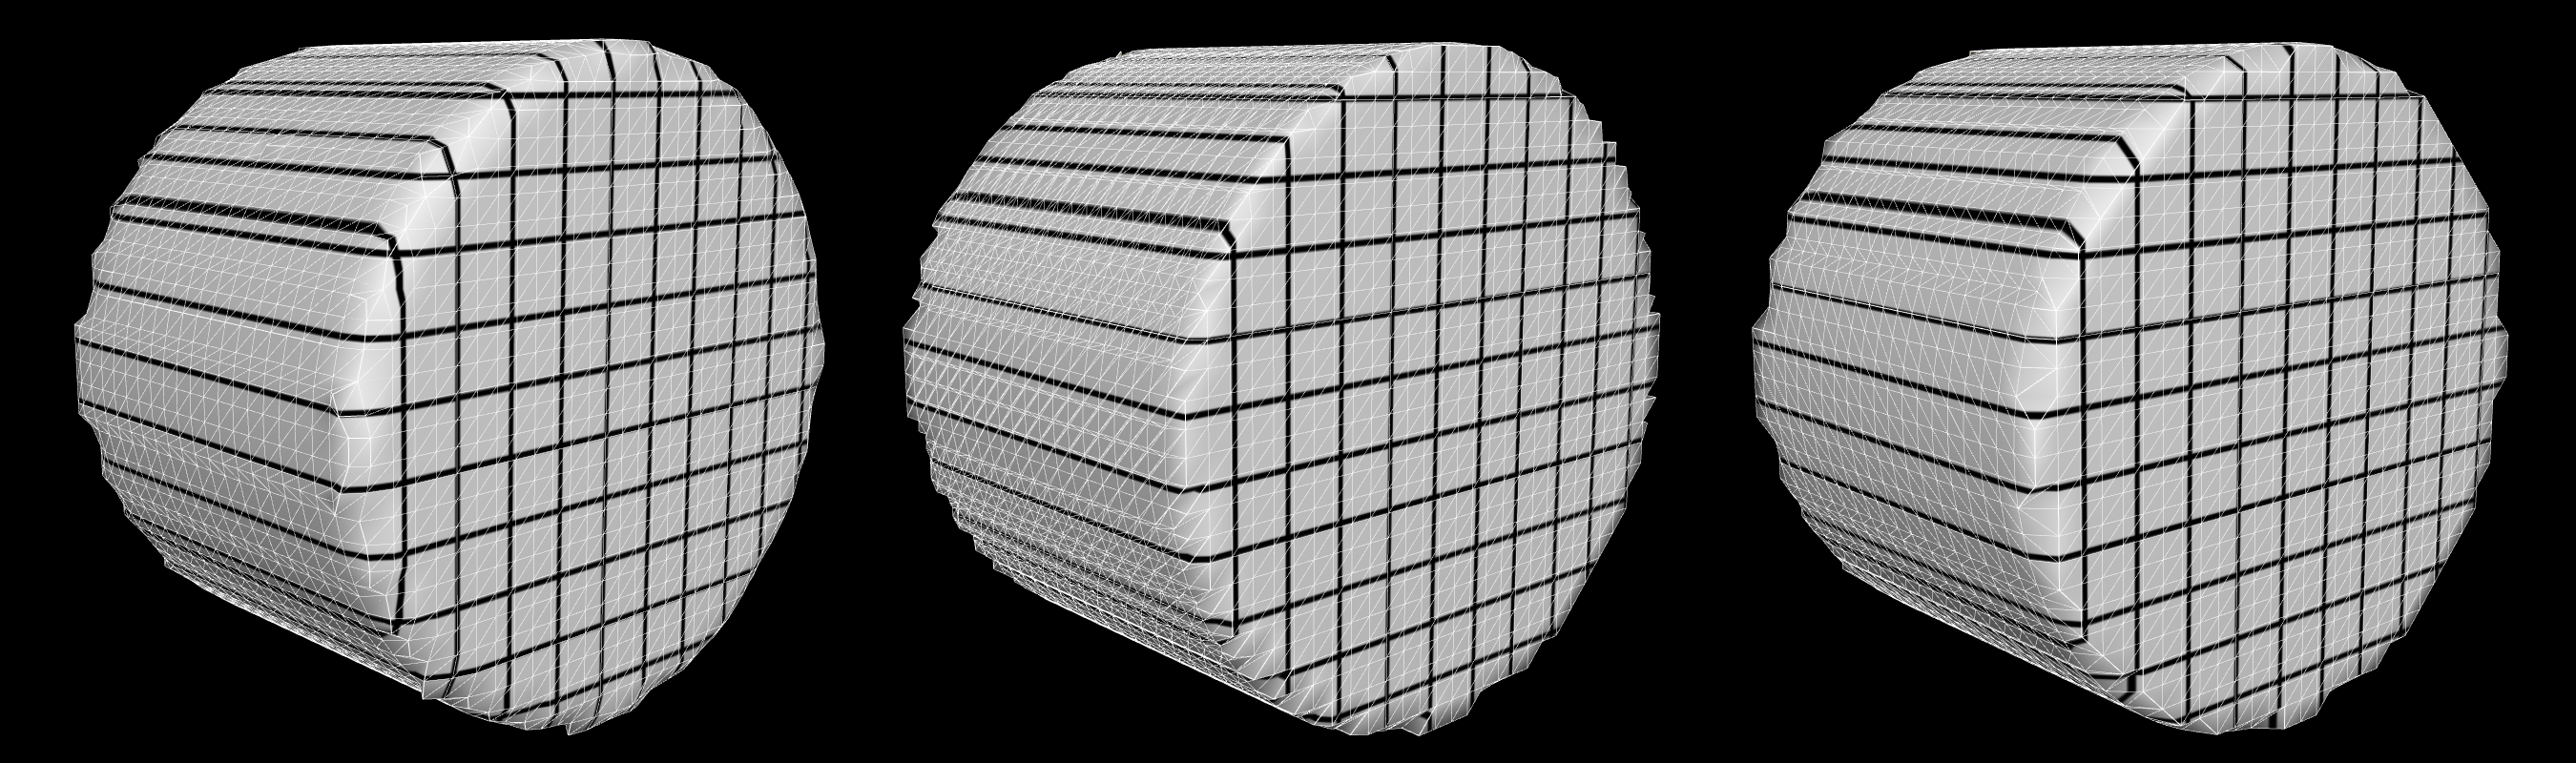
\includegraphics[width=\linewidth,center]{compec3.png}
\caption{Cilindro generado utilizando los 3 algoritmos.}
\end{figure}
\\Se puede apreciar en el cilindro arriba a la izquierda como Marching Tetrahedra genera una superficie más suave.
\clearpage
De forma análoga a la sección anterior, luego se ejecutaron las mismas pruebas pero en lugar de fijando el paso haciendolo con la cantidad de caras, es decir manteniendo la cantidad de caras generadas por cada algoritmo relativamente iguales.
\\Primero se generó la esfera, utilizando 0.05 como paso para Marching Cubes y Naive Surface Nets; mientras que 0.085 para Marching Tetrahedra.
\begin{table}[h!]
  \centering
  \label{tab:table1}
  \begin{tabular}{cccc}
    \toprule
    & Surface Nets & Marching Tetrahedra & Marching Cubes\\
    \midrule
    Cantidad de vértices & 1472 & 9480  & 5880 \\
    Cantidad de caras &  2940 & 3160 & 2936 \\
    \bottomrule
  \end{tabular}
  \caption{Comparación de cantidad de caras y vértices de la esfera utilizando los 3 algoritmos.}
\end{table}
\begin{figure}[h!]
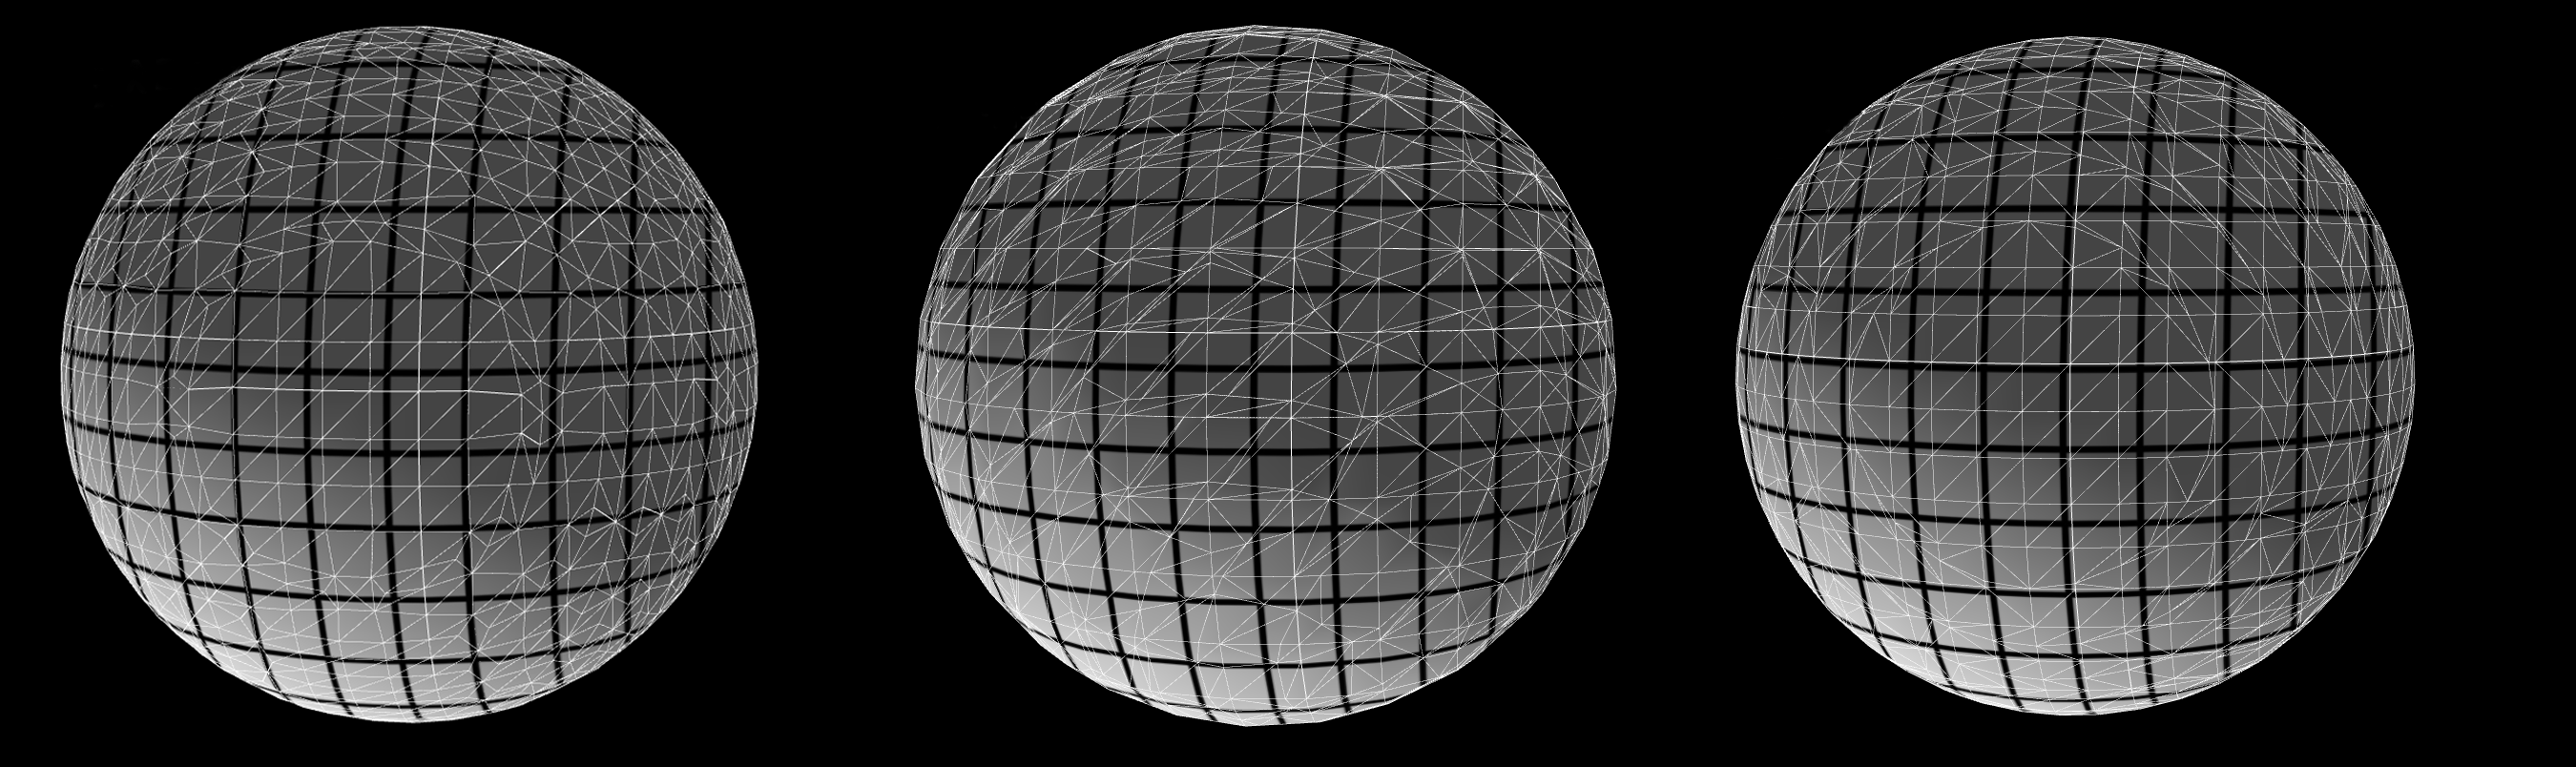
\includegraphics[width=\linewidth,center]{esfera2.png}
\caption{Esfera generada utilizando los 3 algoritmos.}
\end{figure}
\\Es notorio la peor aproximación de Marching Tetrahedra, se puede notar en el sector superior izquierdo.
\\Luego se generó la segunda ecuación, utilizando 0.05 como paso para Marching Cubes y Naive Surface Nets; mientras que 0.085 para Marching Tetrahedra.
\begin{table}[h!]
  \centering
  \label{tab:table1}
  \begin{tabular}{cccc}
    \toprule
    & Surface Nets & Marching Tetrahedra & Marching Cubes\\
    \midrule
    Cantidad de vértices & 23432 & 144408  & 94368 \\
    Cantidad de caras &  47184 & 48136 & 47504 \\
    \bottomrule
  \end{tabular}
  \caption{Comparación de cantidad de caras y vértices de la segunda ecuación utilizando los 3 algoritmos.}
\end{table}
\clearpage
\begin{figure}[h!]
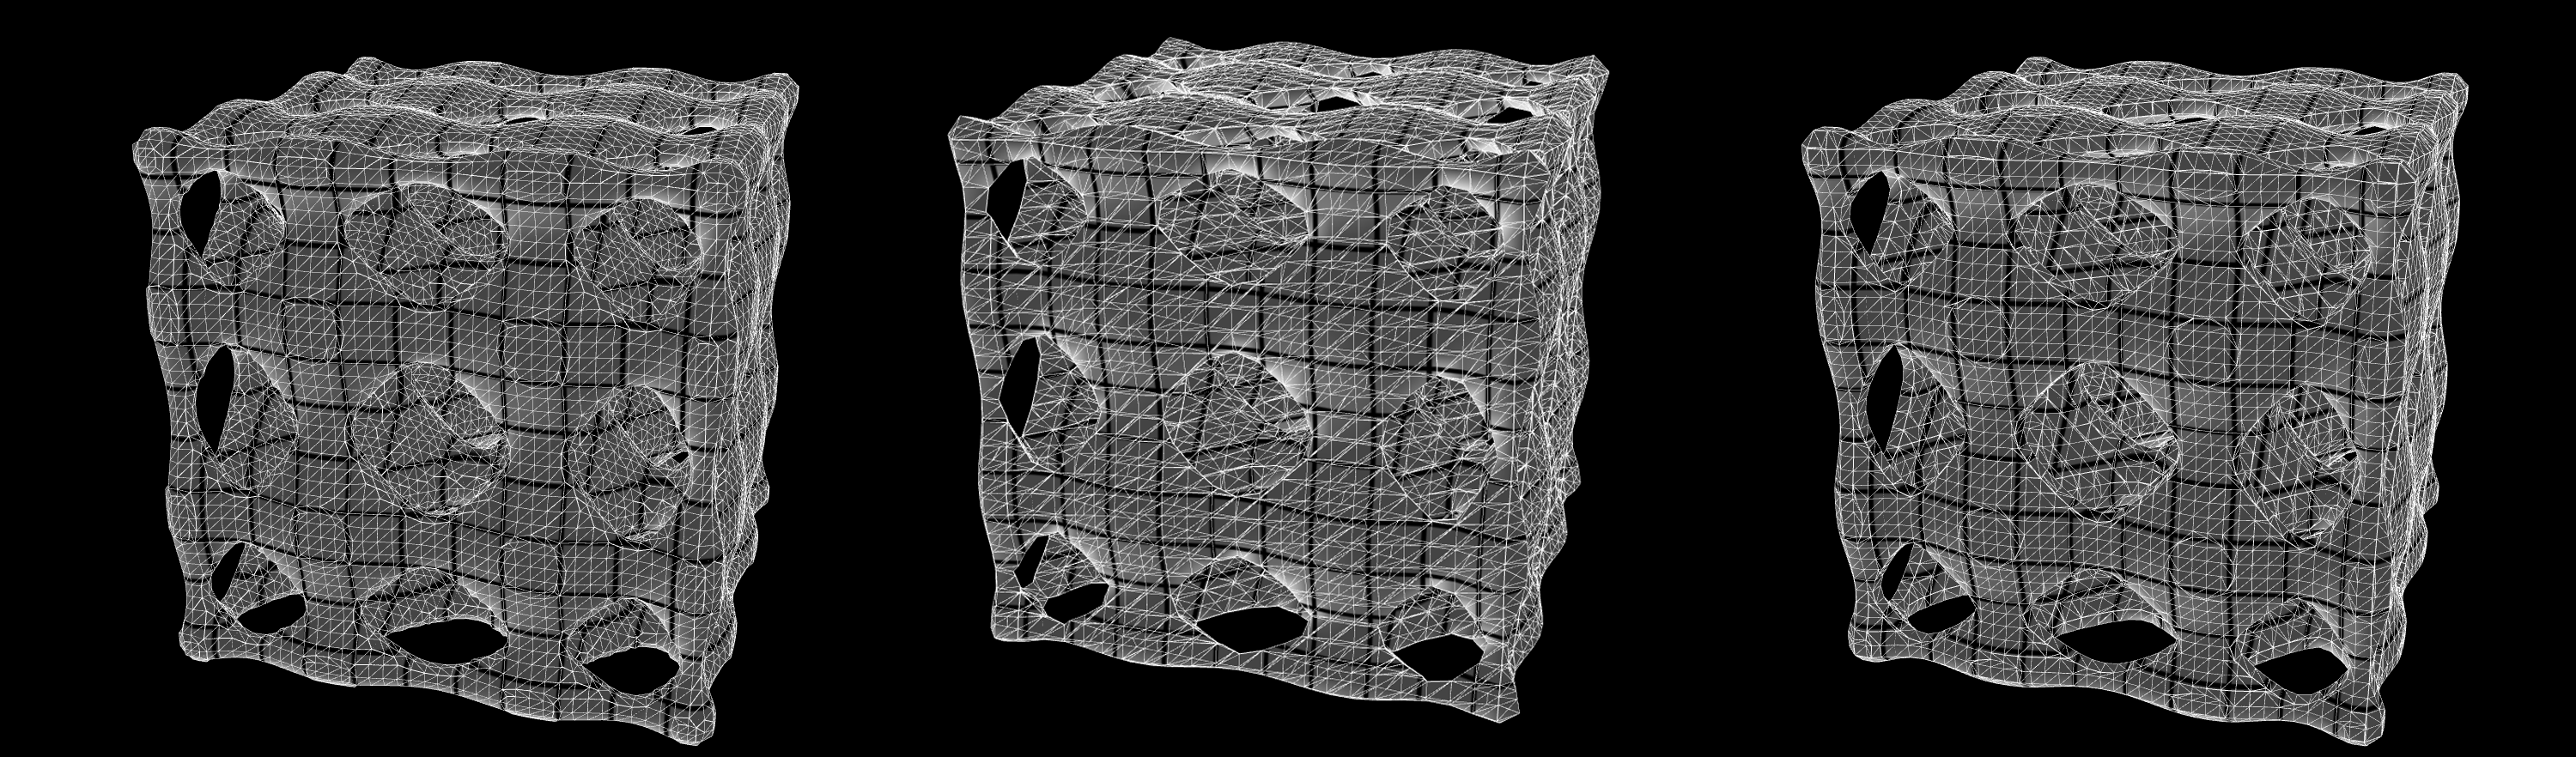
\includegraphics[width=\linewidth,center]{ecuacion2.png}
\caption{Ecuación generada utilizando los 3 algoritmos.}
\end{figure}
En el sector inferior se aprecia una peor aproximación en Marching Tetrahedra.
\\Por último se generó el cilindro, utilizando 0.05 como paso para Marching Cubes y Naive Surface Nets; mientras que 0.085 para Marching Tetrahedra.
\begin{table}[h!]
  \centering
  \label{tab:table1}
  \begin{tabular}{cccc}
    \toprule
    & Surface Nets & Marching Tetrahedra & Marching Cubes\\
    \midrule
    Cantidad de vértices & 14150 &  95624 & 56592 \\
    Cantidad de caras &  28296 & 30208 & 28292 \\
    \bottomrule
  \end{tabular}
  \caption{Comparación de cantidad de caras y vértices del cilindro utilizando los 3 algoritmos.}
\end{table}
\begin{figure}[h!]
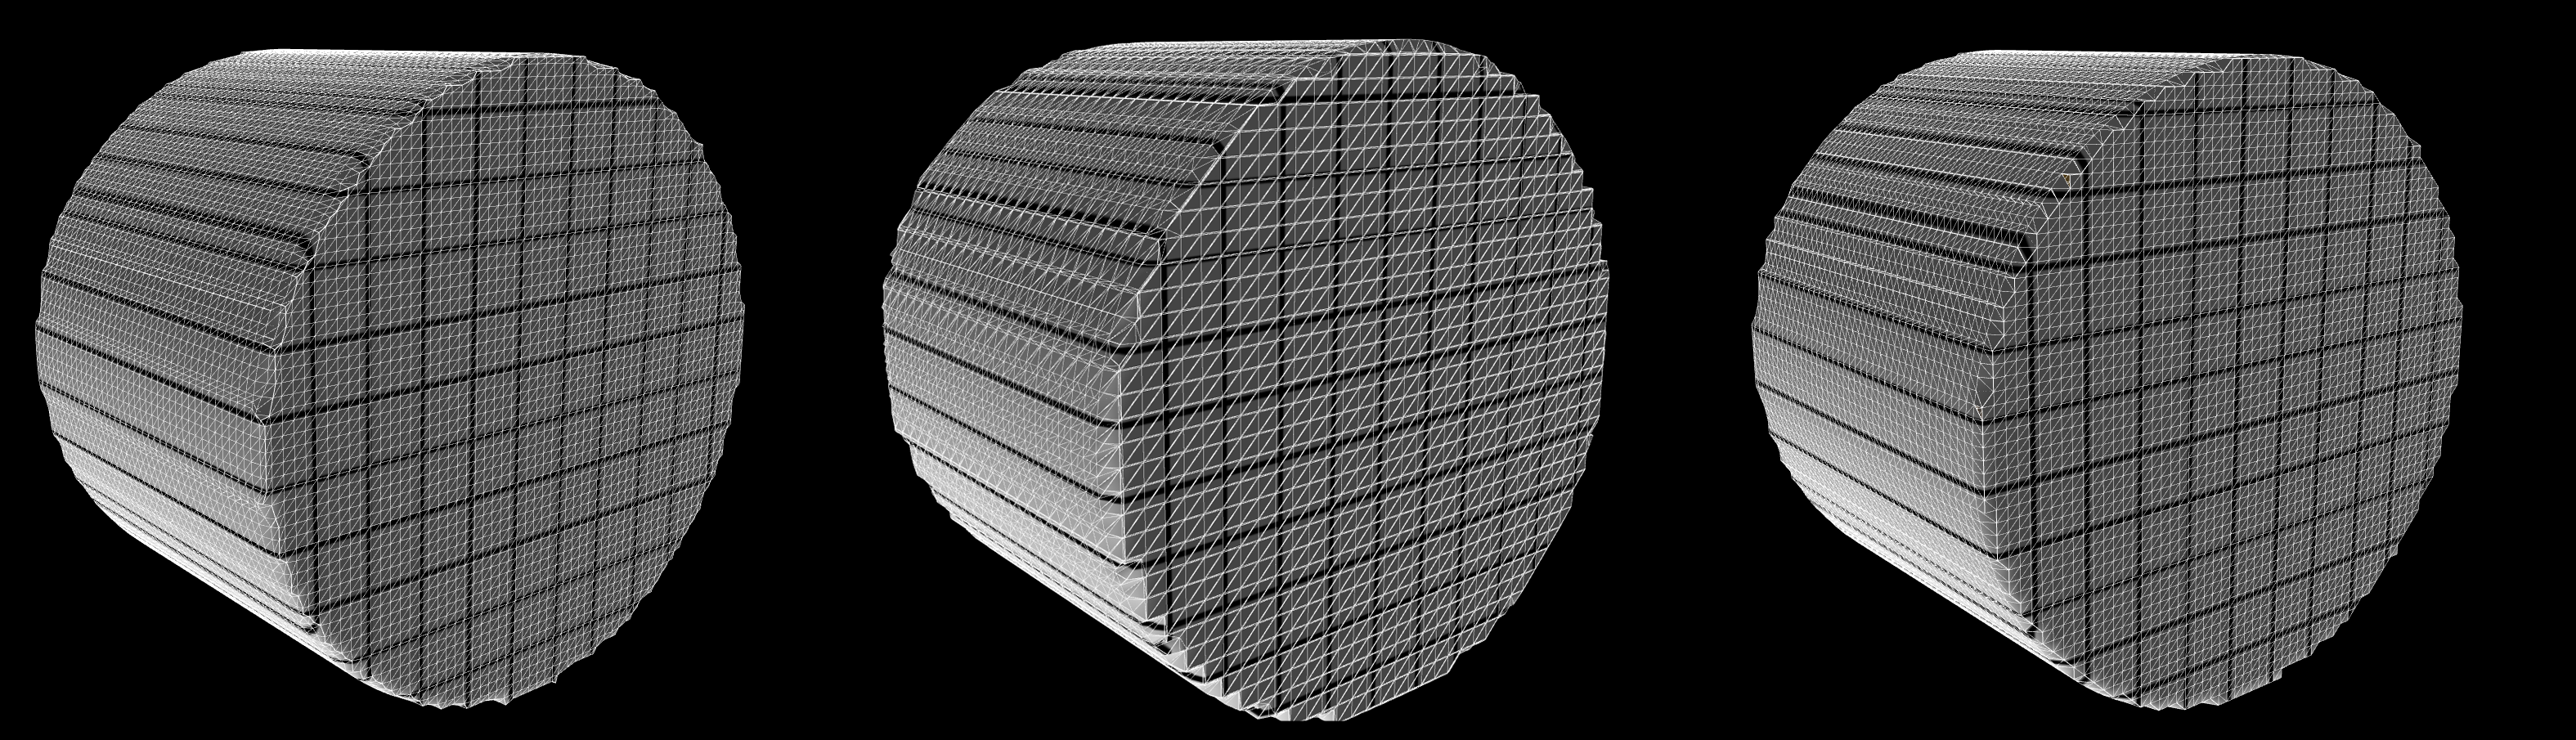
\includegraphics[width=\linewidth,center]{cilindro2.png}
\caption{Cilindro generado utilizando los 3 algoritmos.}
\end{figure}
\\En el sector inferior se aprecia una peor aproximación en Marching Tetrahedra.
\\En estas pruebas se puede apreciar que el algoritmo Marching Tetrahedra cuando se utiliza el mismo paso genera aproximaciones levemente mejores, ya que son más suaves que las obtenidas con los otros dos algoritmos. Por otro lado es el más lento de los tres y genera una mayor cantidad de vértices y caras. Naive Surface Nets es el más rápido de los tres, y las mallas que generan son un poco inferiores a las de Marching Cubes, pero considerando su velocidad es una buena opción. Además de que sus geometrías son las más pequeñas, por lo que se ahorra en memoria. Marching Cubes se ubica en el medio entre los algoritmos, ya que no es el más rápido pero tampoco el más lento, y sus aproximaciones no son las mejores pero tampoco las peores.
\\ A igual cantidad de caras, se puede notar que Marching Tetrahedra es inferior, ya que sus mallas son de peor calidad. Esto se debe a que al tener un paso distinto recibe menos información de laa función ya que la misma se discretiza considerando el paso. Cuando se fija la cantidad de caras, se puede apreciar que Marching Tetrahedra se vuelve más rápido que Marching Cubes en algunos escenarios, pero no que Naive Surface Nets.

\subsection{ Estudio de framerate}
Para realizar un análisis del framerate se colocaron distintas ecuaciones y se registró el framerate promedio luego de 1 minuto de rotar la cámara alrededor de ellas. A continuación se presenta una tabla con la cantidad de caras de la ecuación y el framerate promedio obtenido en Nightly. La resolución de la pantalla es de 1920x1080p.
\begin{table}[h!]
  \centering
  \label{tab:table1}
  \begin{tabular}{cc}
    \toprule
    Cantidad de caras & Framerate promedio (fps)\\
    \midrule
    14304 & 473\\
    79006 & 225\\
    51788 & 289\\
    40886&409\\
    776&695\\
    2797432&77\\
    \bottomrule
  \end{tabular}
  \caption{Comparación entre la cantidad de caras de la ecuación y framerate obtenido.}
\end{table}
\\Estas pruebas se realizaron generando solo un punto de vista, por lo que en modo VR, el framerate sería menor. Aún así la mayoría de las pruebas poseen resultados muy superiores a los 120$fps$ (60Hz es la velocidad de refresco del DK1). Utilizando esto como refencia la única escena que generaría problemas es la de casi tres millones de triángulos.
\subsection{Comparación con SURFER en puntos singulares}
Los puntos singulares presentan inconvenientes para los algoritmos presentados. A continuación presentaremos una serie de imágenes para comparar los resultados que se obtienen utilizando Surfer con nuestra aplicación. 
\\Para hacerlo se utilizará una ecuación con 216 puntos singulares.\\
\begin{figure}[h!]
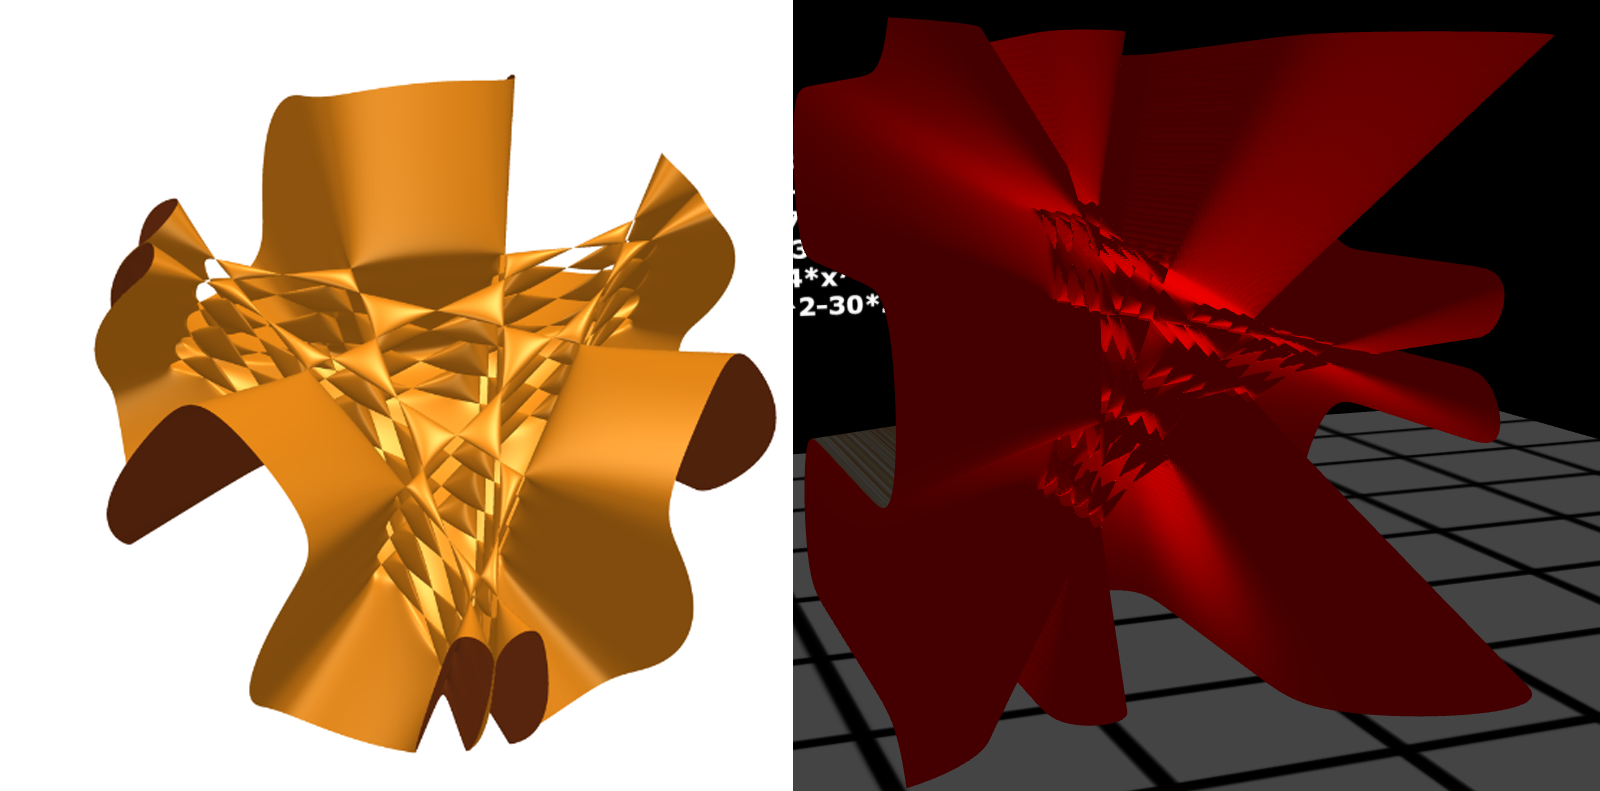
\includegraphics[width=\linewidth]{comp1.png}
\caption{Comparación de una figura con 216 puntos singulares utilizando SURFER y la aplicación desarrollada.}
\end{figure}
\\En la figura 30 a la izquierda se puede apreciar la imagen generada con Surfer y a la derecha la imagen generada con Marching Tetrahedra en nuestra aplicación. Se puede apreciar como Surfer resuelve los puntos singulares de mejor forma. También se puede apreciar como nuestra aplicación posee sombras.
\begin{figure}[h!]
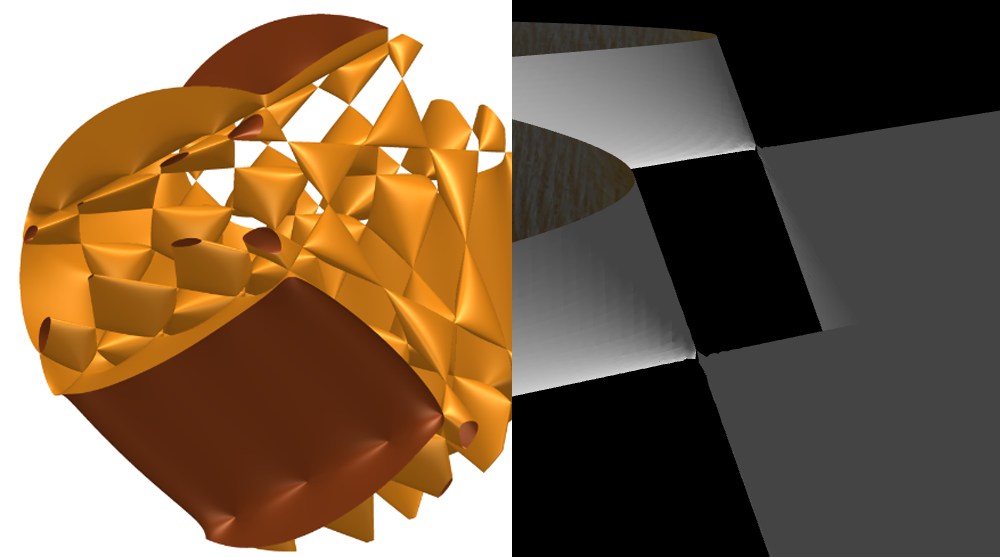
\includegraphics[width=\linewidth]{comp2.png}
\caption{Comparación cuando se realiza zoom hacia un punto singular de la figura anterior.}
\end{figure}
\\Se aprecia a la izquierda de la figura 31 como se visualiza cuando se utiliza el zoom de SURFER, y a la derecha lo que sucede si se utiliza la herramienta de corte para realizar un recálculamiento de la zona problemática. 
\\De estas pruebas se desprende que los puntos singulares son problematicos, y que los resultados obtenidos no son tan buenos como los de SURFER, pero si se quiere visualizar esa zona en particular se puede recalcuar con mayor calidad obteniendo resultados de una calidad similar a la de SURFER.
\clearpage
\subsection{Composición de ecuaciones}
La aplicación desarrollada puede ser utilizada con fines pedagógicos. En esta sección se muestran algunas formas de utilizar el programa para motivar a jóvenes a realizar ecuaciones de forma sencilla e intuitiva, de manera de atraerlos al mundo de la matemática.
\\Una manera interesante de utilizar este software es utilizar la matemática para generar objetos conocidos del mundo real, es decir objetos cotidianos como un tornillo. Una forma de lograr esto es por medio de la unión, intersección y resta de superficies. Esta aplicación puede lograr cada uno de las 3 operaciones de 3 formas distintas.
\\Estas tres operaciones permiten una increíble flexibilidad, y se pueden aprovechar para generar una gran cantidad de superficies. Con estas operaciones se pueden generar todos los cuerpos platónicos, un cilindro con “tapa”, el anillo de Saturno, un tornillo, etc. A continuación se muestran algunos ejemplos.\\
\begin{wrapfigure}{l}{0.4\textwidth}
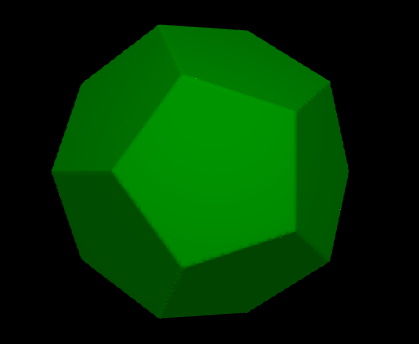
\includegraphics[width=0.9\linewidth]{dodecaedro.png} 
\caption{Dodecaedro generado con la aplicación desarrollada.}
\label{fig:subim1}
\end{wrapfigure}
\\Se pueden ver dos ecuaciones generadas con nuestra aplicación con las operaciones expresadas anteriormente. Particularmente se puede apreciar un dodecaedro, que fue realizado intersectando 12 semiespacios definidos por planos y un tornillo generado a través de la resta entre un cilindro  y una ecuación similar a un resorte.
\\
\\
\\
\\
\\
\\
\\

\begin{figure}[h]
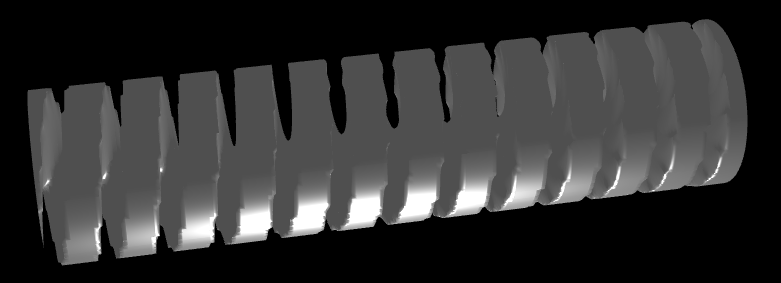
\includegraphics[width=0.7\linewidth,center]{tornillo.png}
\caption{Tornillo generado con la aplicación desarrollada.}
\end{figure}
\clearpage
\subsubsection{Unión de ecuaciones}
Supongamos que contamos con dos superficies $f(x,y,z)=0$ y $g(x,y,z)=0$ (para lo que sigue se asume a que el interior de las ecuaciones es negativo y el exterior positivo), si se quiere generar  $\cup(f,g)$ se puede realizar de 3 modos. 
\\En el primer modo se le resta a la suma la resta del valor absoluto, es decir $\cup(f,g) =  f(x,y,z) + g(x,y,z) - |f(x,y,z) - g(x,y,z)|$. 
 En el segundo caso se le resta a la suma la raíz cuadrada de la suma de los cuadrados de las funciones  $\cup(f,g) = f(x,y,z) + g(x,y,z) -\sqrt[2]{f^2(x,y,z) + g^2(x,y,z)}$.
\\En el tercer tipo se toma el mínimo de las dos  $\cup(f,g)=min(f(x,y,z),g(x,y,z))$
\begin{figure}[h]
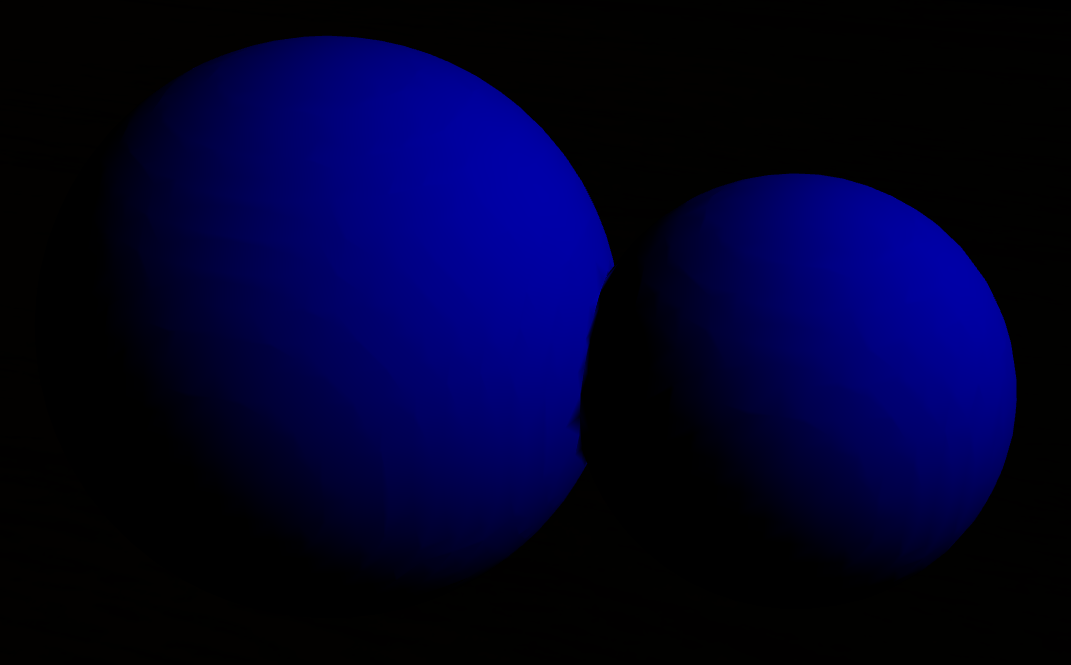
\includegraphics[width=0.7\linewidth,center]{oi1.png}
\caption{Unión de dos esferas generada con la aplicación desarrollada.}
\end{figure}

\subsubsection{Intersección de ecuaciones}
Supongamos que se cuenta con dos superficies iguales a las del punto anterior y se desea intersectar, es decir calcular $\cap(f,g)$. A continuación se listan tres métodos.
\\Este método consiste en sumarle a la suma el valor absoluto de la resta  $\cap(f,g)= f(x,y,z) + g(x,y,z)+ |f(x,y,z) - g(x,y,z)|$ 
\\El segundo método consiste en sumarle a la suma la raíz cuadrada de la suma de los cuadrados de las funciones   $\cap(f,g)= f(x,y,z) + g(x,y,z)+ \sqrt[2]{f^2(x,y,z) +g^2(x,y,z)}$ 
\\El tercer método es tomar el máximo de las dos   $\cap(f,g)= max(f(x,y,z) , g(x,y,z))$
\begin{figure}[h]
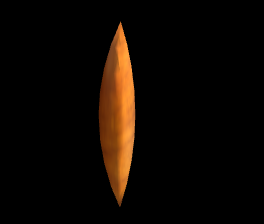
\includegraphics[width=0.7\linewidth,center]{oi2.png}
\caption{Intersección de dos esferas generada con la aplicación desarrollada.}
\end{figure}

\subsubsection{Resta de ecuaciones}
Nuevamente supondremos que contamos con dos superficies f y g que cumplen lo mismo que las anteriores, esta vez obtendremos la diferencia entre ellas, $diff(f,g)$.
\\La primer opción consiste en sumarle a la resta el valor absoluto de la suma $diff(f,g) = f(x,y,z) - g(x,y,z) + |f(x,y,z) + g(x,y,z)|$
\\La segunda consiste en sumarle a la resta la raíz cuadrada de la suma de los cuadrados $diff(f,g) = f(x,y,z) - g(x,y,z) + \sqrt[2]{f^2(x,y,z) + g^2(x,y,z)}$ 
\\Finalmente también es posible tomar el máximo entre $f$ y menos $g$, $max(f(x,y,z),-g(x,y,z))$
\begin{figure}[h]
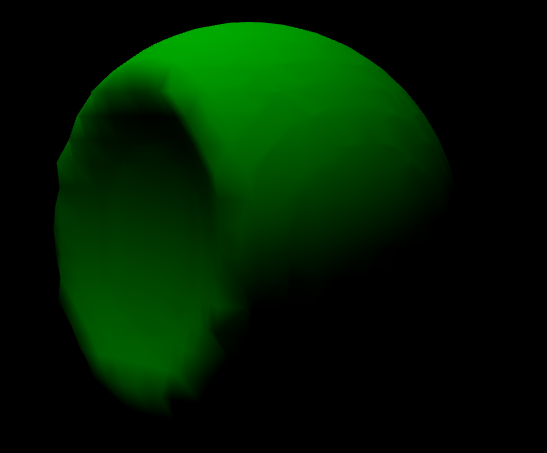
\includegraphics[width=0.7\linewidth,center]{oi3.png}
\caption{Resta de dos esferas generada con la aplicación desarrollada.}
\end{figure}
\clearpage
\subsection{Galería}
En esta sección se muestran una serie de imágenes de superficies generadas con nuestra aplicación, junto con una breve descripción y la ecuación que debe ser ingresada a la aplicación para que se genere la malla.
\\Cubo: $((((x+y+abs(x-y))+(z)+ abs((x+y+abs(x-y))-(z)))+ (-z-2)+abs(((x+y+abs (x-y))+(z)+ abs((x+y+abs(x-y))-(z))) -(-z-2)))+(-x-2)+ abs((((x+y+ abs(x-y))+(z)+ abs((x+y+abs (x-y)) -(z)))+(-z-2) +abs(((x+y+abs(x-y))+(z)+ abs((x+y+ abs(x-y)) -(z)))- (-z-2)))- (-x-2))) + (-y-2) +abs((((( x+y + abs(x-y))+(z)+ abs((x+ y+abs(x-y))-(z)))+(-z-2)+ abs(((x+ y+ abs(x-y))+ (z)+abs((x+y+abs (x-y))-(z)))-(-z-2)))+ (-x-2) +abs((((x+y+abs(x-y))+(z)+ abs((x+y+ abs(x-y))-(z)))+(-z-2)+abs(((x+y+abs(x-y))+(z)+ abs((x+y+abs (x-y))-(z)))-(-z-2)))-(-x-2)))-(-y-2))$
\begin{figure}[h!]
\includegraphics[width=0.7\linewidth,center]{g1.png}
\caption{Cubo generado intersectando 6 semiespacios generados por planos.}
\end{figure}
\clearpage
Cubo con bordes redondeados intersectado con una esfera, al que se le restan 3 cilindros: $((x^6+y^6+z^6-1) +(x^2+y^2+z^2-1.3) +abs((x^6+y^6+z^6-1) -(x^2+y^2+z^2-1.3 ))) -(((y^2+z^2-.5) +(x^2+z^2-.5) -abs((y^2+z^2-.5)-(x^2+z^2-.5))) +(x^2+y^2-.5) -abs(((y^2+z^2-.5)+ (x^2+z^2-.5) - abs ((y^2+z^2-.5) - (x^2+z^2-.5))) -(x^2+y^2-.5))) + abs(((x^6+y^6+z^6-1) +(x^2+y^2+z^2-1.3) + abs((x^6+y^6+z^6-1) -(x^2+y^2+z^2-1.3))) +(((y^2+z^2-.5) +(x^2+z^2-.5)-abs((y^2+z^2-.5)-(x^2+z^2-.5)))+(x^2+y^2-.5)-abs(((y^2+z^2-.5)+(x^2+z^2-.5)-abs((y^2+z^2-.5)-(x^2+z^2-.5)))-(x^2+y^2-.5))))$\\ 
\begin{figure}[h!]
\includegraphics[width=0.7\linewidth,center]{g2.png}
\caption{La resta entre la intersección de una esfera y un cubo con bordes redondeados; y 3 cilindros.}
\end{figure}
\clearpage
Anillo: $max(max(max(y,- (x^2 + y^2 + z^2-1)), -y- 0.01), (x^2 +y^2 +z^2 - 3))$ \\
\begin{figure}[h!]
\includegraphics[width=0.7\linewidth,center]{g3.png}
\caption{Plano que se intersecta con una esfera grande y se le resta una esfera más pequeña.}
\end{figure}
\\Cilindro con tapas: $((x^2/2 + y^2/2 - 1) + (z) + abs((x^2/2 + y^2/2 - 1)-(z)))+(-z-2)+abs(((x^2/2 + y^2/2 - 1) + (z) + abs((x^2/2 + y^2/2 - 1)-(z)))-(-z-2))$ \\
\begin{figure}[h!]
\includegraphics[width=0.7\linewidth,center]{g4.png}
\caption{Intersección de un cilindro con dos planos.}
\end{figure}
\\Tornillo: $max((x^2 + y^2 - 1) ,-((x-sin(z*10) )^2 + (y -cos (z*10))^2 -0.8))$ \\
\begin{figure}[h!]
\includegraphics[width=0.7\linewidth,center]{g5.png}
\caption{Resta entre un cilindro y una ecuación similar a un resorte.}
\end{figure}

\clearpage
\section{Conclusiones y trabajo a futuro}
\subsection{Conclusiones}
Las conclusiones se dividirán en dos partes, en la primera analizaremos la performance de los meshers, comparándolos no sólo entre sí, sino contra raytracing. 
\\En la segunda parte se analizará la performance de la aplicación en cuanto a fps y a resolución de las imágenes generadas. En esta parte se comparará contra Surfer y se analizará si el framerate y la calidad de las imágenes es lo suficientemente bueno para una experiencia positiva de realidad virtual.
\subsubsection{Meshers}
Cada uno de los 3 métodos tiene sus puntos fuertes y débiles. 
\\Marching Cubes es bueno ya que existen implementaciones libres y fácilmente utilizables, y también es bastante rápido. (Sin mencionar que también es la más ampliamente conocida). Además de ser relativamente rápido no tiene el problema de repetir vértices de Naive Surface Nets, y la calidad de las mallas es superior. Los resultados no son tan agradables como los de Marching Tetrahedra, pero es considerablemente más rápido. 
\\Marching Tetrahedra soluciona algunos problemas de Marching Cubes a expensas de ser mucho más lento y la creación de mallas mucho más grandes. Las mallas son más suaves y mejores en general de los tres, pero contiene mucho más vértices y caras, y el algoritmo es mucho más lento.
\\Naive Surface Nets es mucho más rápido y se puede ampliar para generar mallas de alta calidad utilizando algoritmos más sofisticados de selección de vértices. También es fácil de implementar y produce mallas ligeramente más pequeñas. Su inconveniente principal es que las superficies que genera son de peor calidad, aunque podría ser mejorado si se cambia la técnica de elección de vértices. 
\\La elección de cual de los métodos es el superior depende de cada caso, si se quiere ahorrar en memoria y obtener el resultado los más rápido posible, se debe usar Naive Surface Nets, pero asumiendo de que la aproximación puede no ser tan buena como si se utilizase alguno de los otros dos algoritmos. Si se quiere maximizar la precisión de la aproximación se debe utilizar Marching Tetrahedra, pero demorara más tiempo y utilizará más recursos. Finalmente si se quiere una opción más equilibrada, se puede optar por Marching Cubes ya que no es tan preciso a la hora de aproximar como Marching Tetrahedra, pero es más rápido y usa menos recursos; por otra parte es más preciso que Naive Surface Nets pero es más lento. Por este motivo se optó por dejar a Marching Cubes como algoritmo por defecto, pero permitirle al usuario cambiarlo en caso de que este lo considere necesario.
\subsubsection{Calidad de imágen y framerate}
Los framerates obtenidos son altos, son ampliamente superiores a 60 fps (la tasa de refresco que los videojuegos apuntan a obtener). Es también ampliamente superior a los 15 fps que tiene como objetivo mantener el SURFER. Esto hace que la experiencia visual sea muy fluida y agradable (tanto en el modo de realidad virtual como en el normal). 
\\La resolución de las imágenes es alta, los framerates fueron tomados con una pantalla de resolución 1920x1080p, lo que es muy superior a las imágenes que genera SURFER (las cuales no superan 796x796). El hecho de que se pueda mantener un framerate tan alto con esa resolución permite disminuir el efecto de pixelación en Oculus Rift. 
\\El hecho de que se tienen framerates altos y resolución alta, como se dijo anteriormente ayuda a disminuir las probabilidades de que los usuarios experimenten Virtual Reality Sickness. Lo cual es muy positivo ya que permite que la aplicación gane en usabilidad.
\\La experiencia obtenida utilizando la aplicación con DK1 y con DK2 ha sido muy buena, ya que ninguno de los usuarios sufrió ningún tipo de inconveniente, ni sensación de mareo. 
\\Luego de las pruebas con Google Cardboard también fueron favorables, ninguno de los usuarios sufrió ningún tipo de inconveniente.
\\También hay que destacar que aunque se tienen esas ventajas, existe una desventaja con respecto a la utilización de raytracing, la cual es que algunas ecuaciones (particularmente aquellas con muchos puntos singulares) no se visualizan de forma tan precisa, sufriendo algunos artefactos en dichos puntos. Aún así la aproximación es buena, pero la que genera SURFER es superior. También hay que considerar si se utiliza la funcionalidad de cortar y se acerca a las zonas problemáticas el resultado que se obtiene es muy bueno, ya que se disminuye la aparición de la deformación.


\subsection{Trabajo a futuro}
Para mejorar aún más la aplicación se podrían implementar una serie de cambios y agregados. A continuación se listan algunas de ellas.
Agregar a los algoritmos para generar la malla el algoritmo de Dual Contouring\cite{dualcontour}, el cual mejoraría los resultados en cuanto a la calidad de la geometría, aunque sería más lento. 
\\En cuanto a mejorar los algoritmos, se podría implementar diferentes versiones de Surface Nets, es decir cambiar las técnicas de selección de los vértices, utilizar algunas más complejas que obtengan mejores resultados.
\\Agregar otros shaders de GLSL para tener más efectos de ser más atractivo visualmente, se podría permitir a los usuarios agregar sus propios shaders de forma de otorgarles aún un mayor control de cómo se visualiza la ecuación. También se podrían alterar algunos de los ya existentes de manera que los clicks en pantalla afecten el comportamiento de los shaders, por ejemplo que los clicks generen ondas en el agua, o que el movimiento de la ecuación afecte la vibración de la gelatina.
\\Otra mejora sería mejorar la interfaz en caso que se ingrese desde un teléfono, hacerla más amigable para los dispositivos móviles.
También se podrían desarrollar aplicaciones para celular (aprovechando la existencia de herramientas para utilizar HTML, CSS y Javascript para hacer aplicaciones para estos dispositivos) tanto para Android como para iOS. 
\\Se podría traducir el código a C++ utilizando OpenGL, haciendo una versión de escritorio, de esta forma se mejoraría la performance porque se obtendría código compilado además se disminuiría el overhead. Así como se tendría un mayor control del framerate ya que no se dependería del loop de refresco del navegador.
\\Una mejora que se podría realizar es utilizar técnicas de simplificación\cite{simplificacion}\cite{realtimerendering}, con el fin de simplificar la geometría con la menor pérdida de calidad posible. Esto permitiría disminuir considerablemente la cantidad de polígonos en varias de las ecuaciones, por ejemplo si se simplificase la ecuación del plano $x-3=0$ idealmente en lugar de tener una gran cantidad de triángulos dependiendo del paso seleccionado por el usuario, simplemente se tendrían 2.


\clearpage
\section{Glosario}
\textbf{\textit{AngularJS}} es un framework de JavaScript de código abierto, mantenido por Google, que se utiliza para crear y mantener aplicaciones web de una sola página. Su objetivo es aumentar las aplicaciones basadas en navegador con capacidad de Modelo Vista Controlador (MVC), en un esfuerzo para hacer que el desarrollo y las pruebas sean más fáciles.\\
\textbf{\textit{Base de datos}} son bancos de información que contienen datos relativos a diversas temáticas y categorizados de distinta manera, pero que comparten entre sí algún tipo de vínculo o relación que busca ordenarlos y clasificarlos en conjunto\\
\textbf{\textit{Bootstrap}} es un framework o conjunto de herramientas de Código abierto para diseño de sitios y aplicaciones web. Contiene plantillas de diseño con tipografía, formularios, botones, cuadros, menús de navegación y otros elementos de diseño basado en HTML y CSS, así como, extensiones de JavaScript opcionales adicionales.\\
\textbf{\textit{CSS}} en inglés la sigla significa Cascading Style Sheets, es un lenguaje usado para definir y crear la presentación de un documento estructurado escrito en HTML o XML (y por extensión en XHTML). El World Wide Web Consortium (W3C) es el encargado de formular la especificación de las hojas de estilo que servirán de estándar para los agentes de usuario o navegadores.\\
\textbf{\textit{DJANGO}} es un framework de desarrollo web de código abierto, escrito en Python, que respeta el patrón de diseño conocido como Modelo–vista–controlador. Fue desarrollado en origen para gestionar varias páginas orientadas a noticias de la World Company de Lawrence, Kansas, y fue liberada al público bajo una licencia BSD en julio de 2005.\\
\textbf{\textit{FPS}} del inglés frames per second, son la cantidad de imágenes que se muestran en un segundo\\
\textbf{\textit{Git}}  es un software de control de versiones, desarrollado pensando en la eficiencia y la confiabilidad del mantenimiento de versiones de aplicaciones cuando éstas tienen un gran número de archivos de código fuente. Git se ha convertido en un sistema de control de versiones con funcionalidad plena. Hay algunos proyectos de mucha relevancia que ya usan Git.\\
\textbf{\textit{Github}} es una plataforma de desarrollo colaborativo para alojar proyectos utilizando el sistema de control de versiones Git. Utiliza el framework Ruby on Rails por GitHub, Inc. (anteriormente conocida como Logical Awesome). Desde enero de 2010, GitHub opera bajo el nombre de GitHub, Inc. El código se almacena de forma pública, aunque también se puede hacer de forma privada, creando una cuenta de pago.\\
\textbf{\textit{Google Cardboard}} es una plataforma de realidad virtual (VR) desarrollada por Google sobre la base de cartón plegable, de allí su nombre, que funciona a partir de montar un teléfono móvil inteligente con android.\\
\textbf{\textit{GPU}} del inglés Graphics Processing Unit (Unidad de Procesamiento de Gráfico). Es un chip especializado en procesar imágenes en especial gráficos 3D. Su propósito es acelerar cálculos necesarios para dicho procesamiento, se caracterizan por una gran capacidad de procesamiento en paralelo de operaciones numéricas.\\
\textbf{\textit{GLSL}}  es el acrónimo de OpenGL Shading Language (Lenguaje de Sombreado de OpenGL), también conocido como GLslang, una tecnología parte del API estándar OpenGL, que permite especificar segmentos de programas gráficos que serán ejecutados sobre el GPU. Su contrapartida en DirectX es el HLSL. GLSL es un lenguaje de sombreado de alto nivel basado en el lenguaje de programación C.\\
\textbf{\textit{HTML}}  sigla en inglés de HyperText Markup Language (lenguaje de marcas de hipertexto), hace referencia al lenguaje de marcado para la elaboración de páginas web. Es un estándar que sirve de referencia del software que conecta con la elaboración de páginas web en sus diferentes versiones, define una estructura básica y un código (denominado código HTML) para la definición de contenido de una página web, como texto, imágenes, videos, juegos, entre otros. Es un estándar a cargo del World Wide Web Consortium (W3C).\\
\textbf{\textit{JavaScript}} es un lenguaje de programación interpretado, dialecto del estándar ECMAScript. Se define como orientado a objetos, basado en prototipos, imperativo, débilmente tipado y dinámico.\\
\textbf{\textit{Joystick}} es un periférico de entrada de que posee generalmente una o más palancas y varios botones, generalmente se utilizan en los videojuegos.\\
\textbf{\textit{JSON}} acrónimo de JavaScript Object Notation, es un formato de texto ligero para el intercambio de datos. JSON es un subconjunto de la notación literal de objetos de JavaScript aunque hoy, debido a su amplia adopción como alternativa a XML, se considera un formato de lenguaje independiente.\\
\textbf{\textit{Motion sickness}} significa cinetosis en inglés, es la sensación de mareo producida por el movimiento\\
\textbf{\textit{MozVr}} Es el proyecto de Mozilla para agregar la posibilidad de usar realidad virtual en páginas web (WebVR).\\
\textbf{\textit{NodeJS}} es un entorno en tiempo de ejecución multiplataforma, de código abierto, para la capa del servidor (pero no limitándose a ello) basado en el lenguaje de programación ECMAScript, asíncrono, con I/O de datos en una arquitectura orientada a eventos y basado en el motor V8 de Google. Fue creado con el enfoque de ser útil en la creación de programas de red altamente escalables, como por ejemplo, servidores web.\\
\textbf{\textit{Nightly}} es una versión modificada de Mozilla Firefox, la cual cuenta con modificaciones experimentales.\\
\textbf{\textit{Oculus Rift}} es un dispositivo que utiliza técnicas de estereoscopía para poder visualizar en 3D imágenes generadas en las computadoras.\\ 
\textbf{\textit{OpenGL}} es un framework de desarrollo para aplicaciones interactivas con gráficos 2D y 3D. Es soportado por varios sistemas operativos y modelos de tarjetas gráficas.\\
\textbf{\textit{PIP}} es un sistema de gestión de paquetes utilizado para instalar y administrar paquetes de software escritos en Python.\\
\textbf{\textit{PostgreSQL}} es un Sistema de gestión de bases de datos relacional orientado a objetos y libre, publicado bajo la licencia PostgreSQL, similar a la BSD o la MIT.\\
\textbf{\textit{Python}} es un lenguaje de programación interpretado cuya filosofía hace hincapié en una sintaxis que favorezca un código legible.\\
\textbf{\textit{REST}} Transferencia de Estado Representacional (Representational State Transfer) o REST es un estilo de arquitectura software para sistemas hipermedia distribuidos como la World Wide Web. El término se originó en el año 2000, en una tesis doctoral sobre la web escrita por Roy Fielding, uno de los principales autores de la especificación del protocolo HTTP y ha pasado a ser ampliamente utilizado por la comunidad de desarrollo.\\
\textbf{\textit{Renderizar}} es el proceso utilizado para generar una imagen mediante una serie de cálculos partiendo de modelos en 3D\\
\textbf{\textit{Shader}} la tecnología shaders o sombreadores es cualquier unidad escrita en un lenguaje de sombreado que se puede compilar independientemente. Es una tecnología reciente y que ha experimentado una gran evolución destinada a proporcionar al programador una interacción con la unidad de procesamiento gráfico (GPU) hasta ahora imposible. Los shaders son utilizados para realizar transformaciones y crear efectos especiales, como por ejemplo iluminación, fuego o niebla. Para su programación los shaders utilizan lenguajes específicos de alto nivel que permitan la independencia del hardware.\\
\textbf{\textit{SQL}} es en inglés Structured Query Language (lenguaje estructurado de consulta), es un lenguaje utilizado para realizar consultas a la base de datos.\\
\textbf{\textit{THREEJS}} es una librería liviana escrita en JavaScript que permite trabajar con WebGL de forma más sencilla. En este trabajo se utilizó la versión 73.\\
\textbf{\textit{WebGL}} es la versión web de OpenGL, permite la realización de gráficos en 3D en páginas web. Es compatible con la mayoría de los navegadores modernos.\\
\textbf{\textit{XBOX ONE}} consola de videojuegos desarrollada por Microsoft, pertenece a la octava generación de consolas
\clearpage
\section{Referencias}

\begin{thebibliography}{9}

\bibitem{dxplormath} 
3dxplormath organization. homepage. 
Visitado 2016-05-21 
\\\url{http://3d-xplormath.org/}

\bibitem{realtimerendering} 
Akenine-Moller, T., Haines, E., Hoffman, N. (2008). \textit{Real-Time Rendering Third Edition}.

\bibitem{nuestrocodigo} 
Báez, G., Coore, P., (2016), \textit{Implicitus}
\\\url{https://github.com/pablocoore/implicitus}

\bibitem{nuestrositio} 
Báez, G., Coore, P., (2016), \textit{Implicitus}
Visitado 2016-05-29 
\\\url{http://pablocoore.github.io/implicitus/}

\bibitem{marching} 
Bourke, P., (1994) \textit{Polygonising a scalar field},
Descargado 2016-05-27 
\\\url{http://paulbourke.net/geometry/polygonise/}

\bibitem{inter} 
Bourke, P., (1997) \textit{Trilinear Interpolation},
Vistado 2016-05-24 
\\\url{http://paulbourke.net/miscellaneous/interpolation/}

\bibitem{surfacenets} 
Gibson, S., (1999) \textit{Constrained Elastic SurfaceNets: Generating Smooth Models from Binary Segmented Data},
Descargado 2016-05-28 
\\\url{http://www.merl.com/publications/docs/TR99-24.pdf}

\bibitem{implicitas} 
Gomes, A., Voiculescu, I., Jorge, J., Wyvill, B., Galbraith, C., (2009) \textit{Implicit Curves and Surfaces: Mathematics, Data Structures and Algorithms}. 

\bibitem{cardboard} 
Google Cardboard, \textit{homepage},
Visitado 2016-05-15 
\\\url{https://www.google.com/get/cardboard/}

\bibitem{gnuplot} 
Gnuplot. (2016). homepage gnuplot.info. 
Descargado 2016-05-21 
\\\url{http://www.gnuplot.info/}

\bibitem{engine} 
Gregory, J., (2013) \textit{Game Engine Architecture},

\bibitem{htcvive} 
HTC, \textit{HTC Vive},
Visitado 2016-05-19 
\\\url{https://www.htcvive.com}

\bibitem{surfer} 
Imaginary organization. (2016). Surfer. 
Descargado 2016-05-21 
\\\url{https://imaginary.org/es/program/surfer}

\bibitem{usa} 
Johnson, D., (2005), \textit{Introduction to and Review of Simulator Sickness Research (Research Report 1832)}
Descargado 2016-05-19 
\\\url{http://www.dtic.mil/dtic/tr/fulltext/u2/a434495.pdf}

\bibitem{dualcontour} 
Ju, T., Losasso, F., Schaefer, S., Warren, J. (2002). \textit{Dual Contouring of Hermite Data},
Descargado 2016-04-20 
\\\url{http://www.frankpetterson.com/publications/dualcontour/dualcontour.pdf}.

\bibitem{VRS} 
LaViola, J., (2000) \textit{A Discussion of Cybersickness in Virtual Environments},
Descargado 2016-05-30 
\\\url{http://www.eecs.ucf.edu/~jjl/pubs/cybersick.pdf}.

\bibitem{marchingcubes} 
Lorensen, W., Cline, H., (1987)\textit{Marching Cubes: A High Resolution 3D Surface Construction Algorithm},
Descargado 2016-03-25 
\\\url{http://www.cc.gatech.edu/~bader/COURSES/GATECH/CSE6140-Fall2007/papers/LC87.pdf}

\bibitem{simplificacion} 
Luebke, D.,(2001). \textit{A Developer's Survey of Polygonal Simplification Algorithms},
Descargado 2016-05-14
\\\url{http://www.cs.virginia.edu/~luebke/publications/pdf/cg+a.2001.pdf}.

\bibitem{mykola1} 
Lysenko, M., (2012) \textit{Smooth Voxel Terrain (Part 1)},
Visitado 2016-05-22
\\\url{https://0fps.net/2012/07/10/smooth-voxel-terrain-part-1/}

\bibitem{mykola2} 
Lysenko, M., (2012) \textit{Smooth Voxel Terrain (Part 2)},
Visitado 2016-04-03
\\\url{https://0fps.net/2012/07/12/smooth-voxel-terrain-part-2/}

\bibitem{aircraftwing} 
Minh, H., Ngoc, N., Manh, P. (2015). \textit{Aerodynamic Analysis of Aircraft Wing}. 

\bibitem{gamepadapi} 
Mozilla, \textit{Using the Gamepad API},
Visitado 2016-03-20
\\\url{https://developer.mozilla.org/en-US/docs/Web/API/Gamepad_API/Using_the_Gamepad_API#Complete_example_Displaying_gamepad_state}

\bibitem{mozvr} 
Mozilla, \textit{MozVR},
Visitado 2016-04-19
\\\url{https://mozvr.com/}

\bibitem{nightly} 
Mozilla, \textit{Nightly},
Visitado 2016-04-22
\\\url{https://nightly.mozilla.org/}

\bibitem{patterns} 
Nystrom,R \textit{Game Programming Patterns},

\bibitem{oculus} 
Oculus, \textit{homepage},
Visitado 2016-04-28
\\\url{https://www.oculus.com/en-us/rift/}

\bibitem{oculussickness} 
Oculus, \textit{Introduction to Best Practices},
Visitado 2016-05-15
\\\url{https://developer.oculus.com/documentation/intro-vr/latest/concepts/bp	
_intro/}

\bibitem{oculusrendering} 
Oculus, \textit{Rendering to the Oculus Rift},
Visitado 2016-05-20
\\\url{https://developer.oculus.com/documentation/pcsdk/0.5/concepts/dg-render/}

\bibitem{Phong} 
Phong, B. T., (1975). \textit{Illumination for Computer Generated Pictures},
Descargado 2016-05-22
\\\url{http://www.cs.northwestern.edu/~ago820/cs395/Papers/Phong_1975.pdf}.  

\bibitem{samsungvr} 
Samsung, \textit{Samsung VR},
Visitado 2016-05-27
\\\url{http://www.samsung.com/global/galaxy/wearables/gear-vr/}

\bibitem{psvr} 
Sony, \textit{ Playstation VR},
Visitado 2016-05-27
\\\url{https://www.playstation.com/en-au/explore/playstation-vr/}

\bibitem{psvrspecs} 
Sony, \textit{ Playstation VR Tech specs},
Visitado 2016-05-27
\\\url{https://www.playstation.com/en-au/explore/playstation-vr/tech-specs/}

\bibitem{marchingt} 
Tatarchuk, N., Shopf, J., (2007)\textit{Real-Time Medical Visualization with FireGL},
Descargado 2016-05-26
\\\url{http://amd-dev.wpengine.netdna-cdn.com/wordpress/media/2012/10/MedicalVisualization.pdf}

\bibitem{three} 
THREEJS, \textit{homepage},
Visitado 2016-05-26
\\\url{http://threejs.org/}

\bibitem{codigothree} 
THREEJS: THREEJS,
Descargado 2016-03-24
\\\url{https://github.com/mrdoob/three.js/}

\bibitem{shadowmap} 
Williams, L.,(1978). \textit{Casting Curved Shadows on Curved Surfaces},
Descargado 2016-05-26
\\\url{http://people.eecs.berkeley.edu/~ravir/6160/papers/p270-williams.pdf}. 

\end{thebibliography}


\clearpage

\section*{Anexos}
\appendix
\section{Teorema de la función Implícita.}
Dados:
\begin{center}
$F_{1}(x,y,z,u,v,w)=0$\\
$F_{2}(x,y,z,u,v,w)=0$\\
$F_{3}(x,y,z,u,v,w)=0$\\
\end{center}

Si el determinante de la Jacobiana:
\begin{center}
$|J F(u,v,w)|=|\frac{\partial(F_{1},F_{2},F_{3})}{\partial(u,v,w)}|\neq 0$\\
\end{center}
Entonces $u$, $v$ y $w$ pueden ser resueltos en función de $x$,$y$,$z$ y las derivadas parciales de $u$,$v$,$w$ con respecto a $x$,$y$,$z$ se hallan mediante la diferenciación de las mismas.
\clearpage
\section{Cronograma del proyecto}
A continuación se presenta una tabla que muestra las principales actividades realizadas de forma mensual.
\begin{center}
    \begin{tabular}{ | l | p{9cm} |}
    \hline
    Mes &   Tareas \\ \hline
    Septiembre &  Investigación de tecnologías (Java, Oculus Rift, Jovr, JavaFX).\\ & Investigación de SURFER y JSurf. \\ & Estudio de tipos de ecuaciones.\\ \hline
    Octubre &  Inicio de escritura del reporte. \\ & Estudio de visualización estereoscópica \\ & Inicio de prototipo utilizando SURFER. \\ \hline
    Noviembre &  Desarrollo del prototipo utilizando SURFER.\\ & Escritura del reporte. \\ \hline
    Diciembre &  Desarrollo del prototipo utilizando SURFER.\\ & Estudio de VRS.\\ & Escritura del reporte. \\ \hline
    Enero &   Desarrollo del prototipo utilizando SURFER.\\ & Estudio de otras tecnologías (Meshers).\\ &  Evaluación de prototipo SURFER.\\ & Escritura de reporte comparativo.\\ \hline
    Febrero  & Desarrollo de aplicación utilizando Meshers. \\ & Escritura del reporte. \\ \hline
    Marzo &  Desarrollo de la aplicación.\\ & Escritura del reporte. \\ \hline
    Abril &  Desarrollo de la aplicación.\\ & Escritura del reporte. \\ \hline
    Mayo &  Desarrollo de la aplicación.\\ &  Realización de pruebas.\\ & Escritura del reporte. \\ \hline
    Junio &  Desarrollo de la aplicación.\\ &  Realización de pruebas.\\ & Escritura del reporte. \\ \hline
    \hline
    \end{tabular}
\end{center}
\clearpage
\section{Manual de Usuario}
A continuación se presenta un breve manual de usuario, donde se explica como utilizar la aplicación, así como las principales funciones de la misma.
\subsection{Interfaz}
En este punto se muestran los distintos modos con los que se puede interactuar con la aplicación.
\subsubsection{Menú lateral}
Esta interfaz permite varias funcionalidades. En la parte superior se encuentran tres botones, el que se encuentra más a la izquierda oculta el menú inferior, el central activa el modo VR y el de más a la izquierda habilita o deshabilita el uso del teclado para afectar la escena, de modo que ingresar la ecuación no afecte la visualización.
\\El menú lateral está compuesto de varias pestañas que forman un acordeón cada una de éstas representa una ecuación. En cada pestaña se puede elegir:
\begin{wrapfigure}{l}{0.35\textwidth}
\includegraphics[width=0.9\linewidth]{interfaz_lateral.png} 
\caption{Interfaz lateral de la aplicación.}
\label{fig:subim1}
\end{wrapfigure}
\\Si la versión cuenta con la base de datos (es decir si existe conexión con la misma) se puede optar utilizando la lista desplegable por cargar una.
\\Se puede elegir el algoritmo que es utilizado para generar la malla.
\\Se puede elegir si se quiere que se muestren las caras de la figura y/o los edges (aristas) de la misma.
\\Se muestra información útil, como la resolución de la ecuación, la cantidad de vértices y caras.
\\Se muestra la ecuación, la cual puede ser modificada. Se deben ingresar ecuaciones que pueden tener como variables x,y,z; que pueden usar varios tipos de operación entre ellas se encuentran cos, sin, abs, min, max, log, \string^ (potencia).
\\También se encuentra el mínimo/máximo valor de x,y e z.
\\Se encuentra el valor del paso a utilizar en el algoritmo.
\\El botón Update es el responsable de regenerar la geometría utilizando los parámetros ingresados.
\\En un campo se ingresa el nombre, el cual es mostrado arriba en la pestaña, y en caso de estar conectado a la base a la hora de guardar se utilizará ese.
\\Hay un botón que sólo aparece en caso de conexión con la base y permite grabar.
\\Se presentan opciones para cambiar el color interno e externo así como las texturas.
\\Finalmente se encuentra la posición de la figura en la escena.
\\Afuera de las pestañas se encuentra una opción para agregar más ecuaciones (lo que genera más pestañas). 
\\En otro sector se encuentra la configuración del piso. De éste se puede seleccionar, su textura o color, así como si se quiere que sea visible o no.
\\Finalmente se presenta la opción de cambiar el material de la ecuación activa, de cambiar entre el modo de múltiples figuras o no, apagar la luz ambiente y desplegar los ejes de coordenadas de forma de entender mejor la ecuación.
\subsubsection{Mensajes}
Otro aspecto de la interfaz son los mensajes. Estos son pequeños carteles que aparecen arriba la derecha, al momento de ingresar a la página se muestra un mensaje de bienvenida en verde.
\begin{figure}[ht]
\includegraphics[width =0.45\linewidth]{welcome.png}
\hfill
\includegraphics[width =0.45\linewidth]{error.png}
\caption{A la izquierda se muestra el mensaje de bienvenida y a la derecha un ejemplo de mensaje de error.}
\label{ fig : surface }
\end{figure}
\\En caso de que suceda un error en algún momento de la ejecución se muestra un cartel similar pero  rojo, con una descripción del error.
\subsubsection{Teclado y Mouse}
Las funciones del mouse dependerán de en qué modo se encuentre la aplicación:
Si se encuentra en el modo normal, click izquierdo y arrastrar orbita alrededor de la figura,  la rueda del mouse maneja el zoom y el click derecho y arrastrar hace un paneo ya sea lateral o arriba/abajo.
Si se encuentra en modo VR y no se está usando Nightly con un Oculus conectado, en ese caso si se utiliza el click izquierdo y se arrastra se generará una rotación con centro en la posición de la cámara (como si mirase hacia el costado).
\\Para poder utilizar las funcionalidades del teclado, (sin ser escribir la ecuación) se deberá primero activarlas tocando el botón que se mencionó anteriormente.
\\Las siguientes funcionalidades no dependen de si se encuentra en modo VR o no:
\\SHIFT marca la ecuación activa en la escena, colocándole un borde rojo
\\CAPS LOCK le asigna a la ecuación activa el material de agua.
\\TAB le asigna a la ecuación activa el material de lava.
\\P le asigna a la ecuación activa el material de metal.
\\G le asigna a la ecuación activa el material de gelatina.
\\N le asigna a la ecuación activa el material de “Matrix”.
\\Las teclas de la calculadora, 4,6,2,8,7,9 mueven la luz direccional de forma intuitiva.
\\La tecla 1 de la calculadora apaga la luz ambiente.
\\La tecla 3 de la calculadora habilita/deshabilita el “modo cortar” durante este modo + y - agrandan y achican el cubo de corte respectivamente y WASDRF lo mueven en el espacio. La tecla 5 de la calculadora efectúa el corte.
\\La tecla M cambia entre el modo de una única ecuación visible y múltiples.
\\Las teclas del 1 al 0 cambian la ecuación activa. 
\\Durante el modo VR  (siempre que no se esté en el modo cortar) WASDRF  permiten al usuario “caminar” por la escena de modo de explorarla en su totalidad.
\subsubsection{Joystick}
El joystick de XBOX ONE permite cuando se encuentra en modo VR, desplazarse de forma más intuitiva y cómoda que si se utilizase el teclado, ya que se puede conectar de forma inalámbrica.\\
\begin{figure}[h]
\includegraphics[width=0.8\linewidth]{joystick.png}
\caption{Diagrama que muestra el mappeo de las teclas en el joystick.}
\end{figure}
\\Como se puede ver en la imagen anterior se utiliza la palanca izquierda para desplazarse y los dos gatillos (el izquierdo para moverse hacia abajo y el derecho para moverse hacia arriba). A su vez se puede utilizar la palanca derecha para mover la posición de la luz en la escena.
\clearpage
\section{Ejemplo de cómo agregar un nuevo shader}
Este anexo tiene la intención de explicar como sería posible extender la aplicación de forma de agregar otro shader a la misma.
\\A continuación se explica como agregar un vertex shader junto con un fragment shader a la aplicación.
\subsection{Vertex Shader}
Primero se debe programar el vertex shader en GLSL que cuente genere el efecto deseado. Este código debe ser ingresado en el $index.html$ de forma similar a la que se muestra a continuación.
\begin{lstlisting}[frame=single][caption=blabla, label=amb]
<script id="vertexShaderJelly" type="x-shader/x-vertex">
varying vec2 vUv;
uniform float noiseSpeed;
uniform float noiseScale;
uniform float time;
void main() 
{ 
	float displacement = ( vUv.y > 0.999 || vUv.y < 0.001 ) ? 
		 (0.3 + 0.02 * sin(time)) :  
		 sin(time);
    vec3 newPosition = position + vec3(1,0,0) * 
    				displacement*cos(time*position.y/2.0)/10.0;
    vUv = uv;
    gl_Position = projectionMatrix*modelViewMatrix*vec4(newPosition, 1.0);
}
</script>
\end{lstlisting}
El vertex shader es el responsable de retornar en la variable \textit{gl\_Position} la posición del vértice en el espacio homogéneo de cliping (notar que realiza la multiplicación de la matriz de proyección con la de model-view con la posición del punto en el espacio de coordenadas del objeto).
\\Es importante que el id del script sea único y no se repita, ya que se utilizara para referenciarlo desde el MainService.
\clearpage
\subsection{Fragment Shader}
Luego se debe incluir el código del fragment shader en el mismo archivo, a continuación se ve un ejemplo.
\begin{lstlisting}[frame=single][caption=blabla, label=amb]
<script id="fragmentShader" type="x-shader/x-vertex"> 
uniform sampler2D baseTexture;
uniform float baseSpeed;
uniform sampler2D noiseTexture;
uniform float noiseScale;
uniform float alpha;
uniform float time;
varying vec2 vUv;
void main() 
{
	vec2 uvTimeShift = vUv + vec2( -0.7, 1.5 )*time * baseSpeed;	
	vec4 noiseGeneratorTimeShift = texture2D(noiseTexture,uvTimeShift);
	vec2 uvNoiseTimeShift = vUv + noiseScale*
    				vec2(
                    			noiseGeneratorTimeShift.r, 
                    			noiseGeneratorTimeShift.b );
	vec4 baseColor = texture2D( baseTexture, uvNoiseTimeShift );
	baseColor.a = alpha;
	gl_FragColor = baseColor;
}  
</script>
\end{lstlisting}
La función principal del fragment shader es retornar el color del fragmento en \textit{gl\_FragColor}.
\subsection{Función en MainService}
Una vez que se tiene el código en el indice se agrega una función en el MainService y se expone. La función debe generar el material y asignarselo a la ecuación activa. En caso de ser necesario, la función debe cargar los valores iniciales a la $uniform$ que se utilice. La misma se declara global en el MainService. En caso de ser necesario que algún parámetro se recalcule para cada frame, se actualiza el valor dentro de la función $render$ del MainService.
\\A continuación se muestra un ejemplo.
\clearpage
\begin{lstlisting}[frame=single][caption=blabla, label=amb]
var customUniforms;
//continua el modulo
function jellyMaterial(){
	var noiseTexture = 
    		new THREE.ImageUtils.loadTexture('images/cloud.png');
	noiseTexture.wrapS = noiseTexture.wrapT = THREE.RepeatWrapping; 		
	var jellyTexture = 
    		new THREE.ImageUtils.loadTexture('images/jelly.jpg');
	jellyTexture.wrapS = jellyTexture.wrapT = THREE.RepeatWrapping; 
	customUniforms = {
		baseTexture: 	{ type: "t", value: jellyTexture },
		baseSpeed: 		{ type: "f", value: 0.001 },
		noiseTexture: 	{ type: "t", value: noiseTexture },
		noiseScale:		{ type: "f", value: 0.2 },
		alpha: 		{ type: "f", value: 0.5 },
		time: 			{ type: "f", value: 1.0 }
	};
	var customMaterial = new THREE.ShaderMaterial({
	    uniforms: customUniforms,
		vertexShader: document.getElementById('vertexShaderJelly')
        						.textContent,
		fragmentShader: document.getElementById('fragmentShader')
        						.textContent
	});
	customMaterial.side = THREE.DoubleSide;
	customMaterial.transparent = true;
	view.surfacemeshes[view.currentMesh].children[0].material = 
  							customMaterial;
	view.surfacemeshes[view.currentMesh].children[0].material
  							.needsUpdate = true;
	view.surfacemeshes[view.currentMesh].children[1].material = 
   							customMaterial;
	view.surfacemeshes[view.currentMesh].children[1].material
    						.needsUpdate = true;
}

function render() {
	if(customUniforms!=null)
		customUniforms.time.value = clock.getElapsedTime();
//continua la funcion
}
\end{lstlisting}
\clearpage
\section{Ejemplo de cómo agregar un nuevo idioma}
A continuación se presentan cómo y dónde se debería de modificar la aplicación de forma de incluir otro idioma. 
Para lograrlo se debe modificar el archivo $config.js$ de la forma que se muestra a continuación.
\begin{lstlisting}[frame=single][caption=blabla, label=amb]
$translateProvider.translations('en', {
   	//... en ingles  
    }).translations('es', {
        //...                 
    }).translations('ni',{ // 'ni' representa el nuevo idioma
        // se coloca entre comillas simples la traduccion del ingles 
       //de la etiqueta a la izquierda al idioma que se quiere agregar
        ALGORITHM: 'Algorithm', 
        SHOW_FACETS: 'Show facets',
        SHOW_EDGES: 'Show edges',
        VERTEX_COUNT: 'Vertex count',
        FACE_COUNT: 'Face count',
        EQUATION: 'Equation',
        RESOLUTION: 'Resolution',
        UPDATE: 'Update',
        OUTER_TEXTURE: 'Outer texture',
        INNER_TEXTURE: 'Inner texture',
        FLOOR_TEXTURE: 'Floor texture',
        ADD_EQUATION: 'Add equation',
        SHOW_FLOOR: 'Show floor',
        SELECT_MATERIAL: 'Select material',
        MULTIPLE_FIGURES: 'Multiple figures',
        SWITCH_AMBIENT_LIGHT: 'Switch ambient light',
        SHOW_AXES: 'Show axes',
        WELCOME_MESSAGE: 'Welcome to implicitus',
        TOOGLE_KEYBOARD:'Toogle keyboard',
        LOADING:'LOADING',
        LOAD:'Load',
        SAVE:'Save', 
    });
\end{lstlisting}
Luego se debe agregar una función en $controller.js$ que setee el idioma actual a $'ni'$ de manera de que desde 'index.html' pueda modificarse el idioma.
\begin{lstlisting}[frame=single][caption=blabla, label=amb]
$scope.changeLanguageNI=function(){
      $translate.use('ni');
    }
\end{lstlisting}
\clearpage
%este se me ocurrió a mi... si estamos al pedo lo hacemos para llenar el ojo...
\section{Ejemplo de cómo agregar un nuevo algoritmo}
Aquí se explica que pasos debería de seguir un desarrollador que quisiese agregar otro algoritmo para generar la geometría a la aplicación.
\\En caso de querer agregar otro algoritmo, se debe generar un nuevo archivo js, que lo implemente. Ese archivo crear una variable, con el nombre del método, que sea una función que no recibe parámetros, que devuelva otra función que reciba dos parámetros, $data$ y $dims$, y devuelva un objeto con un arreglo de vértices y otro de caras ($vertices$, $faces$). En $data$ se encuentra una discretización de la función y en $dims$ las dimensiones.
\\A continuación se presenta la estructura.
\begin{lstlisting}[frame=single][caption=blabla, label=amb]
var NuevoMetodo = (function() {
return function(data, dims) {   
   var vertices = []
    , faces = [];
    //generar la informacion
  return { vertices: vertices, faces: faces };
}
})();
\end{lstlisting}
Luego es necesario agregar el archivo en $index.html$ y agregar el nombre de la variable a la lista de métodos.
\begin{lstlisting}[frame=single][caption=blabla, label=amb]
meshers = {
    'Marching Cubes': MarchingCubes,
    'Marching Tetraheda' : MarchingTetrahedra,
    'Naive Surface Nets': SurfaceNets,
    'Nuevo Metodo' : NuevoMetodo
};
\end{lstlisting}
\clearpage
\section{Pruebas para los usuarios}
Para cada una de las siguientes pruebas tomamos el tiempo que le llevó a la persona completarla o si fracasó. Además se reportaron comentarios y errores en el uso de la aplicación.
\begin{itemize}
\item Dibuje la ecuación de un plano.
\item Dibuje la ecuación de un plano oblicuo.
\item Dibuje la ecuación de una esfera.
\item Cambie los límites para que se visualice un cuarto de la misma.
\item Asignele una imagen como textura.
\item Utilice el cubo de zoom para visualizar la esfera entera.
\item Entre en modo VR.
\item Asignele un material a la ecuación.
\end{itemize}

\clearpage
\section{Cuestionario de usabilidad de la aplicación}
\textbf{¿Qué le pareció la interfaz de la aplicación?}
\\\\\\\\\\\\
\textbf{¿Le pareció  amigable la forma de ingresar ecuaciones?}
\\\\\\\\\\\\
\textbf{¿Cuál es su opinión sobre la calidad de las superficies mostradas?}
\\\\\\\\\\\\
\textbf{¿Le parecieron interesantes los efectos visuales sobre las superficies?}
\\\\\\\\\\\\
\textbf{¿Sufrío algún tipo de incomodidad o mareo durante el uso de la misma?}
\\\\\\\\\\\\
\textbf{¿Cuál es su opinión general de la aplicación?}
\clearpage
\section{Devolución de los usuarios}
En este anexo se presenta un breve resumen de lo que se obtuvo al presentarle a los usuarios el cuestionario presentado en el anexo anterior.
\end{document}
